%
% Root file for the Programming Guide
% $Id$
%

\documentclass[12pt]{scrbook}

%%%%%%%%%%%%%%%%%%%%%%%%%%%%%%%%%%%%%%%%%%%%%%%%%%%%%%%%%%
%                                                        %
% Uncomment the following if you want to use pdfLaTeX    %
%                                                        %
%%%%%%%%%%%%%%%%%%%%%%%%%%%%%%%%%%%%%%%%%%%%%%%%%%%%%%%%%%

    \usepackage[pdftex]{graphicx}
    \usepackage[pdftex,                %%% hyper-references for pdflatex
    bookmarks=true,                    %%% generate bookmarks ...
    bookmarksnumbered=true,            %%% ... with numbers
    hypertexnames=false,               %%% needed for correct links to figures !!!
    breaklinks=true,                   %%% break links if exceeding a single line
    colorlinks=true,
    citecolor = blue,
    urlcolor = blue]{hyperref}

%%%%%%%%%%%%%%%%%%%%%%%%%%%%%%%%%%%%%%%%%%%%%%%%%%%%%%%%%%
%                                                        %
% Uncomment the follwing, if you want to use plain LaTeX %
%                                                        %
%%%%%%%%%%%%%%%%%%%%%%%%%%%%%%%%%%%%%%%%%%%%%%%%%%%%%%%%%%
%    \usepackage{graphicx}
%    \newcommand{\href}[2]{{\tt #1}}


%%%%%%%%%%%%%%%%%%%%%%%%%%%%%%%%%%%%%%%%%%%%%%%%%%%%%%%%%%
%                                                        %
% Common section for both plain LaTeX and pdfTex         %
%                                                        %
%%%%%%%%%%%%%%%%%%%%%%%%%%%%%%%%%%%%%%%%%%%%%%%%%%%%%%%%%%

\usepackage{a4wide}
\usepackage{times}
\usepackage{fancyhdr}
% Note: next line required to enable longtable to work.
\usepackage{longtable}

\setcounter{secnumdepth}{2}

\sloppy
% page headings

\pagestyle{fancyplain}
\renewcommand{\chaptermark}[1]{\markboth{#1}{#1}}
\renewcommand{\sectionmark}[1]{\markright{\thesection\ #1}}
\lhead[\sf\bfseries\fancyplain{}{\thepage}]{\sf\fancyplain{}{\rightmark}}
\rhead[\sf\fancyplain{}{\leftmark}]{\sf\bfseries\fancyplain{}{\thepage}}
\cfoot{}

\title{JacORB 2.3.1 Programming Guide}

\author{The JacORB Team}

\lowertitleback{{\bfseries Contributors in alphabetical order:}\\
\\
Alphonse Bendt\\
Gerald Brose\\
Nick Cross\\
% appligator removed Sebastian M{\"u}ller\\
Phil Mesnier \\
Nicolas Noffke\\
Steve Osselton\\
Simon McQueen\\
Francisco Reverbel \\
David Robison\\
Andr\'e Spiegel
}

\begin{document}

% uniform formatting of a command line, includes leading $
\newcommand{\cmdline}[1]{\begin{small}\noindent \texttt{\$ #1}\end{small}}

% Use these instead of writing version numbers directly, so
% version changes only have to be made in one place
\newcommand{\JacORBDir}{JacORB2\_3\_1}
\newcommand{\JacORBVersion}{2.3.1}
\maketitle

\setlength{\parskip}{1.1ex}
\newpage
\tableofcontents

%%%%%%%%%%%%%%%%%%%%%%%%%%%%%%%%%%%%%%%%%%%%%%%%%%%%%%%%%%%%%%%%%%%%%%%%%%%%%%

\chapter{Introduction}
\label{ch:intro}

%
% $Id$
%

This document gives an introduction to programming distributed
applications with JacORB, a free Java object request broker. JacORB
comes with full source code, a couple of CORBA Object Service
implementations, and a number of example programs. \\

The JacORB version described in this document is JacORB \JacORBVersion.
The release notes may be found in {\tt <install>/doc/REL\_NOTES}. The current
implementation attempts to conform to the CORBA 3.1 specification.

\section{A Brief CORBA introduction}

CORBA models distributed resources as objects that provide a
well-defined interface. CORBA lets you invoke services through remote
invocations (RPCs). Since the transfer syntax for sending messages to
objects is strictly defined, it is possible to exchange requests and
replies between processes running program written in arbitrary
programming languages and hosted on arbitrary hardware and operating
systems. Target addresses are represented as {\em Interoperable Object
References} (IORs), which contain transport addresses as well as
identifiers needed to dispatch incoming messages to implementations.

Interfaces to remote objects are described declaratively in an
programming language-independent {\em Interface Definition Language}
(IDL), which can be used to automatically generate language-specific
stub code.

It is important to stress that:
\begin{itemize}
\item CORBA objects as seen by clients are abstract entities. Their
  behavior is implemented by artifacts in potentially arbitrary, even
  non-OO languages. These artifacts are called {\em servants} in CORBA
  terminology. A servant is {\em not} the same as the object. Servants
  require an ORB implementation to maintain the relationship to
  objects and to mediate requests and responses.
\item CORBA objects achieve location transparency, i.e., clients need
  not be (and generally are not) aware of the actual target hosts
  where servants reside. However, complete distribution transparency
  is not achieved in the sense that clients would not notice a
  difference between a local function call and a remote CORBA
  invocation. This is due to factors such as increased latency,
  network error conditions, and CORBA-specific initialization code in
  applications, and data type mappings.
\end{itemize}

Please see \cite{Brose2001a,Siegel2000, Vinoski1997} for more
information and additional details, and \cite{Henning1999} for
advanced issues.

\section{Project History}

JacORB originated in 1995 (was it 1996?) in the CS department at Freie
Universit{\"a}t Berlin (FUB). It evolved from a small Java RPC library and a
stub compiler that would process Java interfaces. This predecessor was
written --- most for fun and out of curiosity --- by Boris Bokowski
and Gerald Brose because at that time no Java RMI was available. The
two of us then realized how close the Java interface syntax was to
CORBA IDL, so we wrote an IDL grammar for our parser generator and
moved to GIOP and IIOP as the transport protocol. It was shortly
before Christmas 1996 when the first interoperable GIOP request was
sent form a JacORB client to an IONA Orbix server. For a long time,
JacORB was the only free (in the GNU sense) Java/CORBA implementation
available, and it soon enjoyed widespread interest, at first mostly in
academic projects, but commercial use followed soon after.

For a while, Gerald developed JacORB as a one-man-project until a few
student projects and master theses started adding to it, most notably
Reimo Tiedemann's POA implementation, and Nicolas Noffke's
Implementation Repository and Portable Interceptor implementations.
Other early contributors were Sebastian M{\"u}ller, who wrote the
Appligator, and Herbert Kiefer, who added a policy domain service. The
Appligator and the policy domain service are no longer part of the
JacORB distribution.

A more recent addition is Alphonse Bendt's implementation of the CORBA
Notification Services as part of his master's theses. Substantial additions to
the JacORB core were made by Andr{\'e} Spiegel, who contributed OBV and AMI
implementations. Other substantial contributions to JacORB have been added over
time by the team at PrismTech UK (Steve Osselton, \sout{Nick Cross}, \sout{Simon
McQueen}, Jason Courage)
(\href{http://www.prismtech.com}{http://www.prismtech.com}), Simon McQueen of
MicroFocus (\href{http://www.microfocus.com/products/corba/openfusion/jacorb/index.aspx}),
Nick Cross of Red Hat (\href{http://www.redhat.com}{http://www.redhat.com}) and Phil Mesnier of
OCI (\href{http://www.ociweb.com}{http://www.ociweb.com}). Other active
contributors are Francisco Reverbel of the Red Hat JBoss team (RMI/IIOP)
(\href{http://www.redhat.com}{http://www.redhat.com}) and David Robison, who
contributed CSIv2.

JacORB continues to be used for research at FUB, especially in the
field of distributed object security. A number of people from the original
research group have now left FUB; Gerald is with Projektron BCS
(\href{http://www.projektron.de}{http://www.projektron.de}), Reimo is
with CoreMedia (\href{http://www.coremedia.com}{http://www.coremedia.com}),
Nico and Alphonse worked at Xtradyne (\href{http://www.xtradyne.com}
{http://www.xtradyne.com}) (now part of PrismTech
(\href{http://www.prismtech.com}{http://www.prismtech.com})) and Andr{\'e}
Spiegel is now a free-lance developer and consultant
(\href{http://www.free-software-consulting.com}
{http://www.free-software-consulting.com}).

Due to the limited number of developers, the philosophy around the
development has never been to achieve feature-completeness beyond the
core 90\%, but standards compliance and quality.  (e.g., JacORB 2.0
does not come with a PolicyManager).  Brand-new and less widely-used
features had to wait until the specification had reached a minimum
maturity --- or until someone offered project funding.

\section{Support}

The JacORB core team and the user community together provide best
effort support over our mailing lists.

To enquire about commercial support, please refer to
\href{http://www.jacorb.org/support.html}{http://www.jacorb.org/support.html}.

\section{Contributing --- Donations}

In essence, the early development years were entirely funded by public
research. JacORB did receive some sponsoring over the years, but not
as much as would have been desirable. A few development tasks that
would otherwise not have been possible could be payed for, but more
would have been possible --- and still is.

If you feel that returning some of the value created by the use of
Open Source software in your company is a wise investment in the
future of that the software (maintenance, quality improvements,
further development) in the future, then you should contact us about
donations.

Buying hardware and sending it to us is one option. It is also
possible to directly donate money to the JacORB project at Freie
Universit{\"a}t Berlin. If approval for outright donations is
difficult to obtain at your company, we can send you an invoice for,
e.g., CORBA consulting.

\section{Contributing --- Development}

If you want to contribute to the development of the software directly,
you should do the following:

\begin{itemize}
\item download JacORB and run the software to gain some first-hand
  expertise first
\item read this document and other sources of CORBA documentation,
  such as \cite{Brose2001a}, and the OMG's set of specifications
  (CORBA spec., IDL/Java language mapping)
\item start reading the code
\item subscribe to the {\tt jacorb-developer} mailing list to share
  your expertise
\item contact us to get subscribed to the core team's mailing list and
  send pull requests to the GIT repository.
\item read the coding guide lines
\item contribute code and test cases
\end{itemize}

\section{Feedback, Bug reports}

For limitations, known bugs and bug reporting, please use our Bugzilla
bug tracking system available at
\href{http://www.jacorb.org/bugzilla}{http://www.jacorb.org/bugzilla}.
Please send problems as well as criticism and experience reports to our
developer mailing list available from
\href{http://www.jacorb.org/contact.html}{http://www.jacorb.org/contact.html}.


%%% Local Variables:
%%% mode: latex
%%% TeX-master: "../ProgrammingGuide"
%%% End:


%%%%%%%%%%%%%%%%%%%%%%%%%%%%%%%%%%%%%%%%%%%%%%%%%%%%%%%%%%%%%%%%%%%%%%%%%%%%%%

\chapter{Installing JacORB}
\label{ch:installing}


In this chapter  we explain how to obtain and  install JacORB, and give
an overview of the package contents.

\section{Downloading JacORB}


JacORB can be downloaded as a g-zipped tar--archive or as a zip--archive
from the  JacORB home page  at
\href{http://www.jacorb.org}{http://www.jacorb.org}.

To install JacORB, first unzip  and untar (or simply unzip) the archive
somewhere.  This will result  in a new directory {\tt \JacORBDir}.
After this follow the instructions in {\tt \JacORBDir/doc/INSTALL}.

\section{Installation}
\label{Sec_installation}

\subsection{Requirements}

JacORB requires JDK 1.5 or above properly installed on your machine.  To build
JacORB (and compile the examples) you need to have the XML--based make tool
``Ant'' installed on your machine.  Ant can be downloaded from
\href{http://jakarta.apache.org/ant}{http://jakarta.apache.org/ant}. All make
files ({\tt build.xml}) are written for this tool. To rebuild JacORB
completely, just type {\tt ant} in the installation directory.  Optionally,
you might want to do a {\tt ant clean} first.

For SSL, you need an implementation of the SSL protocol. We currently support
Oracle's JSSE Reference implementation included in the JDK.

\subsection{Dependencies}

JacORB depends upon the following third party software
\begin{enumerate}
\item Simple Logging Facade For Java (SLF4J Version 1.5.0)
\end{enumerate}


%%% Local Variables:
%%% mode: latex
%%% TeX-master: "../ProgrammingGuide"
%%% End:


%%%%%%%%%%%%%%%%%%%%%%%%%%%%%%%%%%%%%%%%%%%%%%%%%%%%%%%%%%%%%%%%%%%%%%%%%%%%%%

\chapter{Configuration}
\label{ch:configuration}

This chapter explains the general mechanism how JacORB is configured,
and lists all configuration properties. Note that ORB configuration
has changed from version 2.1 to 2.2, in particular the names and
locations of the standard configuration files have changed.

\section{Properties}

JacORB has a number of configuration options which can be set as Java
properties. There are three options for setting properties: 

\begin{itemize}
\item properties files
\item command line properties, and 
\item properties passed as arguments to ORB.init() in the code of your
  applications.
\end{itemize}

In the case of a process with multiple ORB instances, it may be
required either to share options between ORBs, or to separate
individual configurations from each other. We explain below how
properties can be set for sharing or for individual ORB instances.

\subsection{Properties files}

JacORB looks for and loads a two standard properties files, a common
file called {\tt common.orb.properties}, and an ORB-specific file one
called {\tt <orbid>.orb.properties}, where  {\tt <orbid>} is the name
of an ORB instance. Also, it can load custom properties files from
arbitrary locations. We explain these files in turn.

\subsubsection{The common properties file}

The reason for having a common properties file is that a single JacORB
installation may be shared by a number of users with a set of common
default, properties. These may be refined by users in their own
properties files but still provide reasonable defaults for the
environment. Note that it is not required to have a common properties
file as all configuration options can also be set in other files, or
on the commandline or in the code.

JacORB looks for the common properties file {\tt
  common.orb.properties} in these places:

\begin{enumerate}
\item in the {\tt lib} directory of the JDK installation. (The JDK's
  home directory denoted by the system property "java.home").
\item in the user home directory. (This is denoted by the system
    property "user.home". On Windows, this is
    {\verb+c:\documents\username+}, on Unixes it's {\verb+~user+}. If
    in doubt where your home directory is, write a small Java programm that
  prints out this property.
\item on the class path.
\end{enumerate}

The common properties file is searched in the order presented above,
so you may actually be loading multiple files of this name. If a
properties file is found, it is loaded, and any property values 
will override values of the same property that were loaded earlier.

Loading properties files from the classpath is useful when
distributing applications packaged in JAR files.

\subsubsection{The ORB properties file}

Having ORB-specific properties files is necessary when multiple ORB
instances live in the same process, but need to have separate
configurations, e.g., some ORBs use SSL and others don't, or some ORBs
need to listen on separate but predefined ports. To let colocated ORBs
use and retrieve separate configurations, JacORB provides an
ORB-specific lookup mechanisms based on a specific property, the {\tt
  ORBid}. (The default value for the ORBid is {\tt jacorb}). To use
different configurations, simply pass different ORBid values to your ORBs.

JacORB looks for ORB properties files in these places:

\begin{enumerate}
\item {\tt jacorb.config.dir/etc/orbid.orb.properties.}, if that exists, or
\item {\tt jacorb.home/etc/orbid.orb.properties.}, or 
\item the current directory ({\tt './orbid.orb.properties.'})
\item on the class path.
\end{enumerate}

The {\tt jacorb.config.dir} and {\tt jacorb.home} properties must be
set for JacORB to be able to use a preconfigured configuration
directory. This can be done in the {\tt common.orb.properties} file,
or by passing a property in on the commandline, like this:

\cmdline{jaco -Djacorb.config.dir=c:/ -DORBid=example test.Example}

The commandline above causes JacORB to look for a file called {\tt
  example.orb.properties} in {\tt c:/etc}. If the {\tt
  -DORBid=example} had been ommitted, the name of the ORB properties
file that JacORB would try to load would have been {\tt
  jacorb.orb.properties}, because that is the default value for the
ORBid. A good starting point is to have a common properties file that
sets the {\tt jacorb.config.dir} property, and then have put a {\tt
  jacorb.orb.properties} file in that directory. Note, however, that
the added flexibility of using multiple configuration files may lead
to individual properties defined in multiple files. You must
know the order in which your configuration files are loaded to avoid
  confusion over property settings not having the expected effect!

\subsubsection{Custom properties files}

In addition to the standard JacORB properties files, a {\em custom
  properties file} can be loaded by passing the name of that
properties files the {\tt custom.props} property to JacORB. This can
be handy for application-specific settings that you want to distribute
with your code, e.g.

The value of this property is the path to a properties file, which
contains the properties you want to load. As an example, imagine that
you usually use plain TCP/IP connections, but in some cases want to
use SSL (see section \ref{ch:SSL}). The different ways of achieving
this are

\begin{itemize}
\item Use just one properties file, but you will have to edit that
  file if you want to switch between SSL and
plaintext connections.
\item Use commandline properties exclusively (cf. below), which may lead to very long
commands
\item Use a command property file for all applications and different
  custom properties files for each application.
\end{itemize}

For example, you could start a JacORB program like this:

\cmdline{jaco -Dcustom.props=c:/tmp/ns.props org.jacorb.naming.NameServer}

In addition to loading any standard properties files found in the
places listed above, JacORB will now also load configuration
properties from the file {\tt c:/tmp/ns.props}, but this last file
will be loaded after the default properties files and its values will
thus take precedence over earlier settings.

\subsection{Command-line properties}

In the same way as the {\tt custom.props} property in the example
above, arbitrary other Java properties can be passed to JacORB
programs using the {\tt -D<prop name>=<prop value>} command line syntax
for the {\tt java} interpreter, but can be used in the same way with
the {\tt jaco} script. Note that in any case the properties must
precede the class name on the command line.

The ORB configuration mechanism will
give configuration properties passed in this way precedence over
property values found in configuration files.

\subsection{Arguments to ORB.init()}

For more application--specific properties, you can pass a {\tt
 java.util.Properties} object to {\tt ORB.init()} during application
initialization. Properties set this way will override properties set
by a properties file. The following code snippet demonstrates how to
pass in a {\tt Properties} object ({\tt args} is the String array
containing command line arguments):

\small{
\begin{verbatim}
    java.util.Properties props = new java.util.Properties();
    props.setProperty("jacorb.implname","StandardNS");
    // use put() under Java 1.1

    org.omg.CORBA.ORB orb = org.omg.CORBA.ORB.init(args, props);
\end{verbatim}
}

\section{Common Configuration Options}

We are now ready to have a look at the most basic JacORB configuration
properties. As a starting point, you should look at the file {\tt
  /etc/jacorb\_properties.template}, which you can adapt to your own
needs.

\subsection{Initial references}

Initial references are object references that are available to CORBA
application through the bootstrap {\tt
  orb.resolve\_initial\_service()} API call. This call takes a string
argument as the name of an initial reference and returns a CORBA
object reference, e.g., to the initial name service.

\renewcommand{\baselinestretch}{0.9}
\small{
\begin{verbatim}
########################################
#                                      #
#   Initial references configuration   #
#                                      #
########################################

#
# URLs where IORs are stored (used in orb.resolve_initial_service())
# DO EDIT these! (Only those that you are planning to use,
# of course ;-).
#
# The ORBInitRef references are created on ORB startup time. In the
# cases of the services themselves, this may lead to exceptions being
# displayed (because the services aren't up yet). These exceptions
# are handled properly and cause no harm!

#ORBInitRef.NameService=corbaloc::160.45.110.41:38693/StandardNS/NameServer-POA/_root
#ORBInitRef.NameService=file:/c:/NS_Ref
ORBInitRef.NameService=http://www.x.y.z/~user/NS_Ref
#ORBInitRef.TradingService=http://www.x.y.z/~user/TraderRef
\end{verbatim}
}
\renewcommand{\baselinestretch}{1.0}
\small\normalsize

The  string value  for  {\tt
ORBInitRef.NameService} is  a URL  for a resource  used to set  up the
JacORB name  server. This URL  will be used  by the ORB to  locate the
file  used to  store  the  name server's  object  reference (see  also
chapter \ref{ch:naming}).

\subsection{Logging}

Beginning with version 2.0, JacORB uses external log kit
implementations for writing logs. The default log kit used by JacORB
is the Apache LogKit implementation. To plug in different loggers, you
need to write code for a custom {\tt LoggerFactory} class yourself and
supply the class name as the value of the {\tt
  jacorb.log.loggerFactory} property. Any new factory needs to
implement the interface {\tt org.jacorb.util.LoggerFactory}.

\subsubsection*{Log levels and different log components}

The JacORB logging mechanism can be fine-tuned to set different log
levels for different components of JacORB. It is still possible to
rely only on one single, default log level. This log level is
specified like this (note that the properties have changed from
previous JacORB versions!):

\renewcommand{\baselinestretch}{0.9}
\small{
\begin{verbatim}
##################################
#                                #
#  Default Logging configuration #
#                                #
##################################

# Name of the factory class that plugs in a given log kit
# The default value is JacORB's own factory for the Apache
# LogKit. Only edit (or uncomment) if you want a different
# log kit.
#jacorb.log.loggerFactory=org.jacorb.util.LogKitLoggerFactory

# log levels:
#
# 0 = fatal errors only = "almost off" (FATAL ERRORS)
# 1 = non-fatal errors and exceptions (ERROR)
# 2 = important messages (WARN)
# 3 = informational messages and exceptions (INFO)
# 4 = debug-level output (DEBUG) (may confuse the unaware user :-)
jacorb.log.default.verbosity=3
\end{verbatim}
}
\renewcommand{\baselinestretch}{1.0}
\small\normalsize

For other components, the individual log levels are set using log
properties specific to that component, e.g.,\\
\\
{\tt jacorb.naming.log.verbosity=0}\\
\\
will turn logging off for the naming service, but all other parts of
the ORB will still use the default log level. The general pattern for
the log level property is {\tt jacorb.<component>.log.verbosity}.
Other components are, e.g., poa, or ssl.

\subsubsection*{Logging output to a file}

The properties specific to file logging are the following:

\renewcommand{\baselinestretch}{0.9}
\small{
\begin{verbatim}
# where does output go? Terminal is default
jacorb.logfile=c:/tmp/jacorb.log

# Append to an existing log file or overwrite? (Applies to
# file logging only)
jacorb.logfile.append=on

# If jacorb.logfile.append is on, set rolling log size in kilobytes.
# A value of 0 implies no rolling log
jacorb.logfile.maxLogSize=0
\end{verbatim}
}
\renewcommand{\baselinestretch}{1.0}
\small\normalsize

Unless the {\tt jacorb.logfile} property is set to a file name, output
will be sent to the terminal. The {\tt jacorb.logfile.append} value
tells the logger whether to overwrite existing log files or to append
to the. The {\tt jacorb.logfile.maxLogSize} property, finally,
determines how large a log file may become before the logger
automatically creates a new file. This value is in kilobytes. If it is
set to 0, log files may become arbitrarily large, no log file rotation
is used.

The  {\tt jacorb.poa.monitoring} property  determines whether  the POA
should bring up a monitoring GUI  for servers that let you examine the
dynamic behavior of  your POA, e.g.  how long  the request queue gets
and whether your thread pool is  big enough.  Also, this tool lets you
change the  state of a POA,  e.g. from {\it active}  to {\it holding}.
Please see chapter \ref{ch:POA} on the POA for more details.


\section{Configuration Properties}

A comprehensive listing and description of the properties which are used
to configure JacORB are given in the following tables.

\begin{small}
\begin{longtable}{|p{5cm}|p{7.5cm}|p{1.5cm}|p{1.5cm}|}
\caption{ORB Configuration}\\
\hline
~ \hfill \textbf {Property} \hfill ~ & ~ \hfill \textbf {Description}
\hfill ~ & ~ \hfill \textbf {Type} \hfill ~ & \hfill \textbf{Default} \endhead
\hline
\verb"ORBInitRef.<service>" & Properties of this form configure
initial service objects which can be resolved via the ORB
resolve\_initial\_references. A variety of URL formats are
supported. & URL & unset \\
\hline
\verb"org.omg.PortableInterc"
\verb"eptor.ORBInitializerCl"
\verb"ass.<name>" & A portable interceptor initializer class
instantiated at ORB creation. & class & unset \\
\hline
\verb"jacorb.orb.objectKeyMa"
\verb"p.<name>" & Maps an object key to an arbitrary string thereby
enabling better readability for corbaloc URLs. & string & \\
\hline

\verb"jacorb.giop_minor_vers"
\verb"ion" & The GIOP minor version number to use for newly created
IORs & integer & 2 \\
\hline
\verb"jacorb.retries" & Number of retries if connection cannot
directly be established & integer & 5 \\
\hline
\verb"jacorb.retry_interval" & Time in milliseconds to wait between
retries & millisec. & 500 \\
\hline
\verb"jacorb.maxManagedBufSi"
\verb"ze" & This is NOT the maximum buffer size that can be used, but
just the largest size of buffers that will be kept and managed. This
value will be added to an internal constant of 5, so the real value in
bytes is 2** (5 + maxManagedBufSize - 1). You only need to increase
this value if you are dealing with LOTS of LARGE data structures. You
may decrease it to make the buffer manager release large buffers
immediately rather than keeping them for later reuse & integer & 18 \\
\hline
\verb"jacorb.bufferManagerFl"
\verb"ushMax" & Whether to use an additional unlimited size buffer
cache for CDROutputStreams. If -1 then off, if zero then this is
feature is enabled, if greater than zero then it is enabled and
flushed every x seconds & integer & -1 \\
\hline
\hline
\verb"jacorb.connection.clie"
\verb"nt.pending_reply_timeo"
\verb"ut" &  Wait the specified number of msecs for a reply to a
request. If exceeded, a org.omg.CORBA.TIMEOUT exception will be
thrown. Not set by default & millisec. & 0  \\
\hline
\verb"jacorb.connection.clie"
\verb"nt.idle_timeout" & Client-side timeout. This is set to non-zero in order
to stop blocking after specified number of milliseconds & millisec. &
unset \\
\hline
\verb"jacorb.connection.clie"
\verb"nt.timeout_ignores_pen"
\verb"ding_messages" & Controls if client-side idle timeouts take care of
pending messages or not. & boolean & \\
\hline
\verb"jacorb.connection.clie"
\verb"nt.retry_on_failure" & Controls if network failures on existing connections
should yield a COMM\_FAILURE or should trigger a remarshaling
of all pending messages. & boolean & \\
\hline
\verb"jacorb.connection.serv"
\verb"er.timeout" & Maximum time in milliseconds that a server keeps a
connection open if nothing happens & millisec. & unset \\
\hline
\verb"jacorb.connection.max"
\verb"_server_transports" & This property sets the
  maximum number of TCP/IP connections that will be listened on by the
  server--side ORB & integer & unlimited \\
\hline
\verb"jacorb.connection.wait"
\verb"_for_idle_interval" & This property sets the
  interval to wait until the next try is made to find an idle connection to
  close & millisec & 500\\
\hline
\verb"jacorb.connection.sele"
\verb"ction_strategy_class" & This property sets
  the {\tt Selection\-Strategy} & class & \\
\hline
\verb"jacorb.connection.stat"
\verb"istics_provider_class" & This property sets
  the {\tt Statistics\-Provider} & class & \\
\hline
\verb"jacorb.connection.del"
\verb"ay_close" & This property controls the behaviour after sending a GIOP
CloseConnection messsage. If set to ``on'', the TCP/IP connection won't be
closed directly. Instead, it is waited for the client to do so
first & boolean & off \\
\hline
\hline
\verb"jacorb.transport.facto"
\verb"ries" & This property controls which transport plug-ins are
available to the ORB.  The value is a list of classes that implement the ETF
{\tt Factories} interface.
& comma-separated list of classes & \\
\hline
\verb"jacorb.transport.serve"
\verb"r.listeners" & Controls which transports should be offered by
JacORB on the server side.  The value is a list of numeric profile
tags for each transport that should be available on the server side.
& comma-separated list of integers & \\
\hline
\verb"jacorb.transport.clien"
\verb"t.selector" & Name of a class that selects the transport profile
to use for communication on the client side.  The value is the fully
qualified name of a class that implements {\tt
  org.jacorb.orb.ProfileSelector}.
& class & \\
\hline
\verb"jacorb.reference_cachi"
\verb"ng" & Whether or not JacORB caches objects references & boolean & unset  \\
\hline
\verb"jacorb.hashtable_class" & The following property specifies the
class which is used for reference caching. WeakHashtable uses
WeakReferences, so entries get garbage collected if only the Hashtable
has a reference to them. This is useful if you have many references to
short-living non-persistent CORBA objects. It is only available for
java 1.2 and above. On the other hand the standard Hashtable keeps the
references until they are explicitly deleted by calling
\_release(). This is useful for persistent and long-living CORBA
objects & class & Hashtable \\
\hline
\verb"jacorb.use_bom" & Use GIOP 1.2 byte order markers, since CORBA
2.4-5 & boolean & off  \\
\hline
\verb"jacorb.giop.add_1_0_pr"
\verb"ofiles" & Add additional IIOP 1.0 profiles even if using IIOP
1.2 & boolean & off \\
\hline
\verb"jacorb.dns.enable" & Use DNS names in IORs, rather than numeric
IP addresses & boolean & off \\
\hline
\verb"jacorb.compactTypecode"
\verb"s" & Whether to send compact typecodes. Options are 0 (off), 1
(Partial compaction), 2 (full compaction of all optional parameters) & integer & 2 \\
\hline
\verb"jacorb.cacheTypecodes" & Whether to cache read
typecodes  & boolean & off \\
\hline
\verb"jacorb.cachePoaNames" & Whether to cache scoped poa
names & boolean & off \\
\hline
\verb"jacorb.interop.indirec"
\verb"tion_encoding_disable" & Turn off indirection encoding for
repeated typecodes. This fixes interoperability with certain broken
ORB's eg. Orbix 2000 & boolean & off \\
\hline
\verb"jacorb.interop.comet" & Enable additional buffer length checking
and adjustment for interoperability with Comet CORBA/COM bridge which
can incorrectly encode buffer lengths & boolean & off
\\
\hline
\verb"jacorb.interop.lax_"
\verb"boolean_encoding" & Treat any non zero CDR encoded boolean value
as true (strictly should be 1 not non zero) & boolean & off \\
\hline
\verb"org.omg.PortableInterc"
\verb"eptor.ORBInitializerCl"
\verb"ass.bidir_init" & This portable interceptor must be configured
to support bi-directional GIOP & class & unset \\
\hline
\verb"jacorb.ior_proxy_host" & The jacorb.ior\_proxy\_host and
jacorb.ior\_proxy\_port properties inform the ORB what IP/port IORs
should contain, if the ServerSockets IP/port can't be used (e.g. for
traffic through a firewall). WARNING: this is just
‘dumb’ replacing, so you have to take care of your
configuration!  & node & unset \\
\hline
\verb"jacorb.ior_proxy_port" & See jacorb.ior\_proxy\_host above &
port & unset \\
\hline
\verb"OAIAddr" & The Object Adapter Internet Address: IP address on
multi-homed host (this gets encoded in object references). NOTE:
Addresses like 127.0.0.X will only be accessible from the same
machine!  & node & unset \\
\hline
\verb"OAPort" & See OAIAddr above & port & unset \\
\hline
\verb"org.omg.PortableInterc"
\verb"eptor.ORBInitializerCl"
\verb"ass.standard_init" & Standard portable interceptor. DO NOT
REMOVE. & class &  \\
\hline
\verb"jacorb.net.socket_fact"
\verb"ory" & Sets or defines the socket factory that must implement
the operations defined in the org.jacorb.orb.factory.SocketFactory
interface. & class & \\
\hline
\verb"jacorb.net.server_sock"
\verb"et_factory" & Sets or defines the socket factory that must
implement the operations defined in the
org.jacorb.orb.factory.ServerSocketFactory interface. & class & \\
\hline
\verb"jacorb.net.socket_fact"
\verb"ory.port.min" & Sets the minimum port number that can be used
for an additional supported socket factory. This property is used in
conjunction with the jacorb.net.socket\_factory.port.max
property. These properties enable the factory to traverse firewalls
through a fixed port range  & integer & unset (disabled) \\
\hline
\verb"jacorb.net.socket_fact"
\verb"ory.port.max" & Sets the maximum port number that can be used
for the additional supported socket factory. Refer to
jacorb.net.socket\_factory.port.min above & integer & disabled\\
\hline

\end{longtable}
\end{small}


\begin{small}
\begin{longtable}{|p{5cm}|p{7.5cm}|p{1.5cm}|p{1.5cm}|}
\caption{Logging Configuration}\\
\hline
~ \hfill \textbf {Property} \hfill ~ & ~ \hfill \textbf {Description}
\hfill ~ & ~ \hfill \textbf {Type} \hfill ~ & ~ \hfill
\textbf{Default} ~ \endhead
\hline
\verb"jacorb.orb.print_versi"
\verb"on" & If enabled, the ORB's version number is printed whenever
the ORB is initialized. & boolean & on \\
\hline
\verb"jacorb.log.logger" & Name of the logger factory class, can be
used & class & {\tiny \verb"org.jacorb.util" }\\
\verb"LogFactory" & to plug in different log implementationas &  & {\tiny \verb"LogKitLoggerFactory" }\\
\hline
\verb"jacorb.log.default."
\verb"verbosity" & Log levels: 0 = fatal errors, 1 =
error, 2 = warning, 3 = info, 4 = debug & integer & 0 \\
\hline
\verb"jacorb.logfile" & Output destination for diagnostic log file. If
not set, diagnostics are sent to standard error. & filename & unset \\
\hline
\verb"jacorb.logfile.append" & Whether to append to
existing log file or overwrite (if file logging) & boolean & off \\
\hline
\verb"jacorb.logfile.maxLogS"
\verb"ize" & If appending to a file sets the size in kilobytes at
which the file is rolled over & integer & 0 \\
\hline
\verb"jacorb.debug.dump_outg"
\verb"oing_messages" & Hex dump outgoing messages & boolean & off \\
\hline
\verb"jacorb.debug.dump_inco"
\verb"ming_messages" & Hex dump incoming messages & boolean & off \\
\hline
\end{longtable}
\end{small}


\begin{small}
\begin{longtable}{|p{5cm}|p{9cm}|p{2cm}|}
\caption{Appligator Configuration}\\
\hline
~ \hfill \textbf {Property} \hfill ~ & ~ \hfill \textbf {Description} \hfill ~ & ~ \hfill \textbf {Type} \hfill ~ \endhead
\hline
\verb"jacorb.ProxyServer.URL" & This is the URL for the default Appligator and is used when applets or firewall traversal is supported via the JacORB Appligator.  & URL \\
\hline
\verb"jacorb.ProxyServer.URL"
\verb"-<network>-<netmask>" & Additional appligators can be configured for remote subnets using this subnet form of URL configuration. The subnet for a scoped appligator is calculated by the logical ANDing of the network and netmask values.  & URL \\
\hline
\verb"jacorb.ProxyServer.Nam"
\verb"e" & The name the appligator uses when adding itself to the Name Service (if available) on start up. Default is Appligator. & string \\
\hline
\verb"jacorb.ProxyServer.ID" & Defines the object identity for the appligator IOR. If not set, then this defaults to 'Appligator': it is recommended that this is set to some other value for additional security. & string \\
\hline
\verb"jacorb.ProxyServer.Net"
\verb"mask" & Optionally used to configure the network for the local client. When used, the calls to objects within the local subnet will not be redirected. Not set by default. & IP address \\
\hline
\verb"jacorb.ProxyServer.Net"
\verb"work" & See jacorb.ProxyServer.Netmask above. Not set by default. & IP address \\
\hline

\end{longtable}
\end{small}


\begin{small}
\begin{longtable}{|p{5cm}|p{9cm}|p{2cm}|}
\caption{POA Configuration}\\
\hline
~ \hfill \textbf {Property} \hfill ~ & ~ \hfill \textbf {Description} \hfill ~ & ~ \hfill \textbf {Type} \hfill ~ \endhead
\hline
\verb"jacorb.poa.monitoring" & Displays a GUI monitoring tool for servers. Default is off. & boolean \\
\hline
\verb"jacorb.poa.thread_pool"
\verb"_max" & Maximum thread pool configuration for request processing & integer \\
\hline
\verb"jacorb.poa.thread_pool"
\verb"_min" & Minimum thread pool configuration for request processing & integer \\
\hline
\verb"jacorb.poa.thread_prio"
\verb"rity" & If set, request processing threads in the POA will run at this priority. If not set or invalid, MAX\_PRIORITY will be used. Not set by default. & integer \\
\hline
\verb"jacorb.poa.queue_wait" & Specifies whether the POA should block
when the request queue is full (On), or throw TRANSIENT exceptions
(Off). Default is Off. & boolean\\
\hline
\verb"jacorb.poa.queue_max" & The maximum length of the request
queue.  If this length has been reached, and further requests arrive,
jacorb.poa.queue\_wait specifies what to do. Default is 100. & integer \\
\hline
\verb"jacorb.poa.queue_min" & If jacorb.poa.queue\_wait is On, and the
request queue gets full, then the POA blocks until the queue contains
no more than queue\_min requests. Default is 10. & integer \\
\hline

\end{longtable}
\end{small}


\begin{small}
\begin{longtable}{|p{5cm}|p{9cm}|p{2cm}|}
\caption{Implementation Repository Configuration}\\
\hline
~ \hfill \textbf {Property} \hfill ~ & ~ \hfill \textbf {Description} \hfill ~ & ~ \hfill \textbf {Type} \hfill ~ \endhead
\hline
\verb"jacorb.use_imr" & Switch on to contact the Implementation Repository (IR) on every server start-up. Default is off. & boolean \\
\hline
\verb"jacorb.use_imr_endpoin"
\verb"t" & Switch off to prevent writing the IMR address into server IORs. This property is ignored if jacorb.use\_imr = off. Default is off. & boolean \\
\hline
\verb"jacorb.imr.allow_auto_"
\verb"register" & If set to on servers that don't already have an entry on their first call to the IR, will get automatically registered. Otherwise, an UnknownServer exception is thrown. Default is off. & boolean \\
\hline
\verb"jacorb.imr.check_objec"
\verb"t_liveness" & If set on the IR will try to ping every object reference that it is going to return. If the reference is not alive, then TRANSIENT is thrown. Default is off. & boolean \\
\hline
\verb"ORBInitRef.Implementat"
\verb"ionRepository" & The initial reference for the IR. & URL \\
\hline
\verb"jacorb.imr.table_file" & File in which the IR stores data. & file \\
\hline
\verb"jacorb.imr.backup_file" & Backup data file for the IR. & file \\
\hline
\verb"jacorb.imr.ior_file" & File to which the IR writes its IOR. This is usually referred to by the initial reference for the IR (configured above).  & file \\
\hline
\verb"jacorb.imr.timeout" & Time in milliseconds that the implementation will wait for a started server to register. After this timeout is exceeded the IR assumes the server has failed to start. Default is 12000 (2 minutes). & millisec. \\
\hline
\verb"jacorb.imr.no_of_poas" & Initial number of POAs that can be registered with the IR. This is an optimization used to size internal data structures. This value can be exceeded. Default is 100. & integer \\
\hline
\verb"jacorb.imr.no_of_serve"
\verb"rs" & Initial number of servers that can be registered with the IR. This is an optimization used to size internal data structures. This value can be exceeded. Default is 5. & integer \\
\hline
\verb"jacorb.imr.port_number" & Starts the IMR on a fixed port (equivalent to the -p option). & integer \\
\hline
\verb"jacorb.imr.connection_"
\verb"timeout" & Time in milliseconds that the IR waits until a connection from an application client is terminated. Default is 2000. & millisec. \\
\hline
\verb"jacorb.implname" & The implementation name for persistent servers. Persistent servers should set this to a unique name. This is the service name that is registered in the IR. & name \\
\hline
\verb"jacorb.java_exec" & Command used by the IR to start servers. & command \\
\hline

\end{longtable}
\end{small}


\begin{small}
\begin{longtable}{|p{5cm}|p{9cm}|p{2cm}|}
\caption{Security Configuration}\\
\hline
~ \hfill \textbf {Property} \hfill ~ & ~ \hfill \textbf {Description} \hfill ~ & ~ \hfill \textbf {Type} \hfill ~ \endhead
\hline
\verb"OASSLPort" & The port number used by SSL, will be dynamically assigned by default. & port \\
\hline
\verb"org.omg.PortableInterc"
\verb"eptor.ORBInitializerCl"
\verb"ass.ForwardInit" & Portable interceptor required to support SSL. Not set by default. & class \\
\hline
\verb"jacorb.security.access"
\verb"_decision" & The qualified classname of access decision object. & class \\
\hline
\verb"jacorb.security.princi"
\verb"pal_authenticator" & A list of qualified classnames of principle authenticator objects, separated by commas (no whitespaces.). The first entry (that can be successfully created) will be available through the principal\_authenticator property. & class \\
\hline
\verb"jacorb.ssl.socket_fact"
\verb"ory" & The qualified classname of the SSL socket factory class. & class \\
\hline
\verb"jacorb.ssl.server_sock"
\verb"et_factory" & The qualified classname of the SSL server socket factory class. & class \\
\hline
\verb"jacorb.security.change"
\verb"_ssl_roles" & Exchange SSL client server roles to enforce client authentication. Beware: this causes problems with peers that not prepared to handle this role change. Default is off. & boolean \\
\hline
\verb"jacorb.security.suppor"
\verb"t_ssl" & Whether SSL security is supported. Default is off. & boolean \\
\hline
\verb"jacorb.security.ssl.cl"
\verb"ient.supported_options" & SSL client supported options - IIOP/SSL parameters (numbers are hex values, without the leading 0x): NoProtection = 1, EstablishTrustInClient = 40, EstablishTrustInTarget = 20, mutual authentication = 60. Default is 0. Please see the programming guide for more explanation. & integer \\
\hline
\verb"jacorb.security.ssl.cl"
\verb"ient.required_options" & SSL client required options (See IIOP/SSL parameters above). Default is 0. & integer \\
\hline
\verb"jacorb.security.ssl.se"
\verb"rver.supported_options" & SSL server supported options (See IIOP/SSL parameters above). Default is 0. & integer \\
\hline
\verb"jacorb.security.ssl.se"
\verb"rver.required_options" & SSL server required options (See IIOP/SSL parameters above). Default is 0. & integer \\
\hline
\verb"jacorb.security.ssl.co"
\verb"rbaloc_ssliop.supporte"
\verb"d_options" & Used in conjunction with jacorb.security.ssl.corbaloc\_ssliop.required\_options. If these properties are set, then two values will be placed in the IOR, "corbaloc:ssliop” and "ssliop”. If not set, only EstablishTrustInTarget is used for both supported and required options. & integer \\
\hline
\verb"jacorb.security.ssl.co"
\verb"rbaloc_ssliop.required"
\verb"_options" &  Default is 0. & integer \\
\hline
\verb"jacorb.security.keysto"
\verb"re" & The name and location of the keystore. This may be absolute or relative to the home directory. NOTE (for Sun JSSE users): The javax.net.ssl.trustStore [Password] properties doesn't seem to take effect, so you may want to add trusted certificates to normal keystores. In this case, please set the property jacorb.security.jsse. trustees\_from\_ks to on, so trusted certificates are taken from the keystore instead of a dedicated truststore.  & file \\
\hline
\verb"jacorb.security.keysto"
\verb"re_password" & The keystore password. & string \\
\hline
\verb"jacorb.security.truste"
\verb"es" & Files with public key certificates of trusted Certificate Authorities (CA). WARNING: If no CA certificates are present, the IAIK chain verifier will accept ALL otherwise valid chains. & file \\
\hline
\verb"jacorb.security.defaul"
\verb"t_user" & The name of the default key alias to look up in the keystore. & name \\
\hline
\verb"jacorb.security.defaul"
\verb"t_password" & The name of the default key alias to look up in the keystore. & string \\
\hline
\verb"jacorb.security.iaik_d"
\verb"ebug" & Sets IAIKS SSL classes to print debug output to standard output. Default is off. & boolean \\
\hline
\verb"jacorb.security.jsse.t"
\verb"rustees_from_ks" & Sun JSSE specific settings: Use the keystore to take trusted certificates from. Default is off. & boolean \\
\hline
\verb"jacorb.security.ssl.se"
\verb"rver.cipher_suites" & A comma-separated list of cipher suite names which must NOT contain whitespaces. See the JSSE documents on how to obtain the correct cipher suite strings. & string \\
\hline
\verb"jacorb.security.ssl.cl"
\verb"ient.cipher_suites" & See jacorb.security.ssl.server.cipher\_suites above. & string \\
\hline
\end{longtable}
\end{small}

%%% Local Variables:
%%% mode: latex
%%% TeX-master: "../ProgrammingGuide"
%%% End:


%%%%%%%%%%%%%%%%%%%%%%%%%%%%%%%%%%%%%%%%%%%%%%%%%%%%%%%%%%%%%%%%%%%%%%%%%%%%%%

\chapter{Getting Started}
\label{ch:start}


Before we explain an example in detail, we look at the general process
of developing CORBA applications with JacORB. We'll follow this
roadmap when working through the example.  The example can be found in
{\tt demo/grid} which also contains a build file so that the
development steps do not have to be carried out manually every time.
Still, you should know what is going on.

As this document gives only a short introduction to JacORB programming
and does not cover all the details of CORBA IDL, we recommend that you
also look at the other examples in the {\tt demo/} directory.  These
are organized so as to show how the different aspects of CORBA IDL can
be used with JacORB.

\section{JacORB development: an overview}

The steps we will generally have to take are:

\begin{enumerate}
    \item  write an IDL specification.
    \item compile this specification with the IDL compiler to generate
      Java classes (Java interfaces, helper and holder classes, as
      well as stubs and skeletons).
    \item write an implementation for the Java interface generated in step 2
    \item write a ``Main'' class that instantiates the server implementation
        and registers it with the ORB
    \item write a client class that retrieves a reference to the
    server object and makes remote invocations, i.e. CORBA calls.
\end{enumerate}


\section{IDL specifications}

Our example uses a simple server the definition of which should be
clear if you know IDL. Its interface is given in {\tt server.idl}. All
the source code for this example can be found in {\tt \JacORBDir/demo/grid}.

{\small
\begin{verbatim}
// server.idl
// IDL definition of a 2-D grid:
module demo
{
  module grid
  {
    interface MyServer
    {
        typedef fixed <5,2> fixedT;

        readonly attribute short height;  // height of the grid
        readonly attribute short width;   // width of the grid

        // set the element [n,m] of the grid, to value:
        void set(in short n, in short m, in fixedT value);

        // return element [n,m] of the grid:
        fixedT get(in short n, in short m);

        exception MyException
        {
            string why;
        };

        short opWithException() raises( MyException );
    };
  };
};
\end{verbatim}
}

\section{Generating Java classes}

Feeding this file into the IDL compiler

\cmdline{idl -d ./generated server.idl}

produces a number of Java classes that represent the IDL definitions.
This is done according to a set of rules known as the IDL-to-Java
language mapping as standardized by the OMG. If you are interested in
the details of the language mapping, i.e. which IDL language construct
is mapped to which Java language construct, please consult the
specifications available from {\tt http://www.omg.org}. The language mapping
used by the JacORB IDL compiler is the one defined in CORBA 2.3 and is
explained in detail in \cite{Brose2001a}. For practical usage, please
consult the examples in the {\tt demo} directory.

The most important Java classes generated by the IDL compiler are the
interfaces {\tt MyServer} and {\tt MyServerOperations}, and the stub
and skeleton files {\tt \_MyServerStub, MyServerPOA} and {\tt
  MyServerPOATie}.  We will use these classes in the client and server
as well as in the implementation of the grid's functionality and
explain each in turn.

Note that the IDL compiler will produce a directory structure for the
generated code that corresponds to the module structure in the IDL
file, so it would have produced a subdirectory {\tt demo/grid} in the
current directory had we not directed it to put this directory
structure to {\tt ./generated} by using the compiler's {\tt -d} switch.
  Where to put the source files for generated classes is a matter of
  taste.  Some people prefer to have everything in one place (as using
  the {\tt -d} option in this way achieves), others like to have one
  subdirectory for the generated source code and another for the
  output of the Java compiler, i.e. for the {\tt .class} files.


\section{Implementing the interface}

Let's try to actually provide an implementation of the functionality
promised by the interface. The class which implements that interface
is called {\tt gridImpl}.  Apart from providing a Java implementation
for the operations listed in the IDL interface, it has to inherit from
a generated class that both defines the Java type that represents the
IDL type {\tt MyServer} and contains the code needed to receive remote
invocations and return results to remote callers.  This class is {\tt
  MyServerPOA}.

You might have noticed that this approach is impractical in situations
where your  implementation class needs to inherit  from other classes.
As  Java only has  single inheritance  for implementations,  you would
have  to use  an alternative  approach ---  the  ``tie''--approach ---
here. The tie approach will be explained later.

Here is  the Java code for  the grid implementation. It  uses the Java
library  class  {\tt  java.math.BigDecimal}  for  values  of  the  IDL
fixed--point type {\tt fixedT}:

\small{
\begin{verbatim}
package demo.grid;

/**
 * A very simple implementation of a 2-D grid
 */

import demo.grid.MyServerPackage.MyException;

public class gridImpl
    extends MyServerPOA
{
    protected short height = 31;
    protected short width = 14;
    protected java.math.BigDecimal[][] mygrid;

    public gridImpl()
    {
        mygrid = new java.math.BigDecimal[height][width];
        for( short h = 0; h < height; h++ )
        {
            for( short w = 0; w < width; w++ )
            {
                mygrid[h][w] = new java.math.BigDecimal("0.21");
            }
        }
    }

    public java.math.BigDecimal get(short n, short m)
    {
        if( ( n <= height ) && ( m <= width ) )
            return mygrid[n][m];
        else
            return new java.math.BigDecimal("0.01");
    }

    public short height()
    {
        return height;
    }

    public void set(short n, short m, java.math.BigDecimal value)
    {
        if( ( n <= height ) && ( m <= width ) )
            mygrid[n][m] = value;
    }

    public short width()
    {
        return width;
    }

    public short opWithException()
        throws demo.grid.MyServerPackage.MyException
    {
        throw new demo.grid.MyServerPackage.MyException("This is only a test exception, no harm done :-)");
    }
}
\end{verbatim}
}

\section{Writing the Server}

To actually instantiate a {\tt  gridImpl} object which can be accessed
remotely  as  a CORBA  object  of type  {\tt  MyServer},  you have  to
instantiate it  in a main method  of some other class  and register it
with a  component of the CORBA  architecture known as  the {\it Object
Adapter}. Here is  the class {\tt Server} which  does all that is
necessary to  activate a  CORBA object of  type {\tt MyServer}  from a
Java {\tt gridImpl} object:

\small{
\begin{verbatim}
package demo.grid;

import java.io.*;
import org.omg.CosNaming.*;

public class Server
{
    public static void main( String[] args )
    {
        org.omg.CORBA.ORB orb = org.omg.CORBA.ORB.init(args, null);
        try
        {
            org.omg.PortableServer.POA poa =
                org.omg.PortableServer.POAHelper.narrow(
                     orb.resolve_initial_references("RootPOA"));

            poa.the_POAManager().activate();

            org.omg.CORBA.Object o = poa.servant_to_reference(new gridImpl());

            if( args.length == 1 )
            {
                // write the object reference to args[0]

                PrintWriter ps = new PrintWriter(
                                    new FileOutputStream(
                                       new File( args[0] )));
                ps.println( orb.object_to_string( o ) );
                ps.close();
            }
            else
            {
                // register with the naming service

                NamingContextExt nc =
                     NamingContextExtHelper.narrow(
                        orb.resolve_initial_references("NameService"));
                nc.bind( nc.to_name("grid.example"), o);
            }
        }
        catch ( Exception e )
        {
            e.printStackTrace();
        }
        orb.run();
    }
}
\end{verbatim}
}

After initializing the ORB we need to obtain a reference to the object
adapter --- the POA --- by asking  the ORB for it. The ORB knows about
a few initial references that can be retrieved using simple names like
``RootPOA''. The returned object is  an untyped reference of type {\tt
CORBA.Object} and thus needs to  be narrowed to the correct type using
a static  method {\tt narrow()}  in the helper  class for the  type in
question. We now  have to activate the POA because  any POA is created
in  ``holding''   state  in  which   it  does  not   process  incoming
requests.  After  calling {\tt  activate()}  on  the POA's  POAManager
object, the POA is in an active state and can now be asked to create a
CORBA  object  reference  from a  Java  object  also  know as  a  {\tt
Servant}.

In order to make the newly created CORBA object accessible, we have to
make its  object reference  available. This is  done using  a publicly
accessible directory  service, the naming  server. A reference  to the
naming      service     is      obtained      by     calling      {\tt
orb.resolve\_initial\_references("NameService")}   on   the  ORB   and
narrowing the reference using the {\tt narrow()} method found in class
{\tt org.omg.CosNaming.NamingContextExtHelper}.  Having done this, you
should call the  {\tt bind()} operation on the  name server.  The name
for the object which has to be supplied as an argument to {\tt bind()}
is not simply a string. Rather, you need to provide a sequence of {\tt
CosNaming.NameComponent}s that represent the  name. In the example, we
chose to use an extended Name Server interface that provides us with a
more convenient conversion operation from strings to Names.


\section{Writing a client}

Finally, let's have a look at the client class which invokes the
server operations:

\small{
\begin{verbatim}
package demo.grid;

import org.omg.CosNaming.*;

public class Client
{
   public static void main(String args[])
   {
       try
       {
           MyServer grid;
           org.omg.CORBA.ORB orb = org.omg.CORBA.ORB.init(args,null);

           if(args.length==1 )
           {
               // args[0] is an IOR-string
               grid = MyServerHelper.narrow(orb.string_to_object(args[0]));
           }
           else
           {
               NamingContextExt nc =
                   NamingContextExtHelper.narrow(
                      orb.resolve_initial_references("NameService"));

               grid = MyServerHelper.narrow(
                         nc.resolve(nc.to_name("grid.example")));
            }

            short x = grid.height();
            System.out.println("Height = " + x);

            short y = grid.width();
            System.out.println("Width = " + y);

            x -= 1;
            y -= 1;

            System.out.println("Old value at (" + x + "," + y +"): " +
                               grid.get( x,y));

            System.out.println("Setting (" + x + "," + y +") to 470.11");

            grid.set( x, y, new java.math.BigDecimal("470.11"));

            System.out.println("New value at (" + x + "," + y +"): " +
                               grid.get( x,y));

           try
           {
               grid.opWithException();
           }
           catch (jacorb.demo.grid.MyServerPackage.MyException ex)
           {
               System.out.println("MyException, reason: " + ex.why);
           }
       }
       catch (Exception e)
       {
           e.printStackTrace();
       }
   }
}
\end{verbatim}
}

After  initializing the  ORB, the  client obtains  a reference  to the
``grid''  service by locating  the reference  using the  name service.
Again, resolving the name is done by getting a reference to the naming
service                 by                 calling                {\tt
orb.resolve\_initial\_references("NameService")} and querying the name
server for  the {\tt "grid"}  object by calling {\tt  resolve()}.  The
argument  to  the  resolve  operation  is, again,  a  string  that  is
converted to  a Name. The result  is an object reference  of type {\tt
org.omg.CORBA.Object}  which has  to be  narrowed to  the type  we are
expecting, i.e. {\tt MyServer}.

After compiling everything we're now  ready to actually run the server
and the  client on  different (virtual) machines.  Make sure  the name
server is running before starting  either the server or the client. If
it isn't, type something like:

\cmdline{ns /home/me/public\_html/NS\_Ref}

where  {\tt /home/me/public\_html/NS\_Ref}  is the  name of  a locally
writable file  which can be  read by using  the URL given in  both the
remote client and  server code. (This is to  avoid using a well--known
address for  the name server,  so both client  and server look  up the
location of the  name server via the URL and  later communicate with it
directly.)

You can now launch the server:

\cmdline{jaco demo.grid.Server}

The client can be invoked on any machine you like:

\cmdline{jaco demo.grid.Client}

Running the  client after starting  the server produces  the following
output on your terminal:

\begin{verbatim}
Height = 31
Width = 14
Old value at (30,13): 0.21
Setting (30,13) to 470.11
New value at (30,13): 470.11
MyException, reason: This is only a test exception, no harm done :-)
done.
\end{verbatim}

\subsection{The Tie Approach}

If your implementation class cannot inherit from the generated servant
class  {\tt  MyServerPOA} because,  e.g.,  you  need  to inherit  from
another  base class,  you can  use the  tie approach.  Put  simply, it
replaces  inheritance by  delegation. Instead  of inheriting  from the
generated  base  class, your  implementation  needs  to implement  the
generated {\em operations interface} {\tt MyServerOperations}:

\begin{verbatim}
package demo.grid;

import demo.grid.MyServerPackage.MyException;

public class gridOperationsImpl
    implements MyServerOperations
{
...
}
\end{verbatim}

Your server is then written as follows:

\begin{verbatim}
package demo.grid;

import java.io.*;
import org.omg.CosNaming.*;

public class TieServer
{
    public static void main( String[] args )
    {
        org.omg.CORBA.ORB orb =
            org.omg.CORBA.ORB.init(args, null);
        try
        {
            org.omg.PortableServer.POA poa =
                org.omg.PortableServer.POAHelper.narrow(
                     orb.resolve_initial_references("RootPOA"));

            // use the operations implementation and wrap it in
            // a tie object

            org.omg.CORBA.Object o =
                poa.servant_to_reference(
                     new MyServerPOATie( new gridOperationsImpl()) );

            poa.the_POAManager().activate();

            if( args.length == 1 )
            {
                // write the object reference to args[0]

                PrintWriter ps = new PrintWriter(
                    new FileOutputStream(new File( args[0] )));
                ps.println( orb.object_to_string( o ) );
                ps.close();
            }
            else
            {
                NamingContextExt nc =
                     NamingContextExtHelper.narrow(
                        orb.resolve_initial_references("NameService"));
                NameComponent [] name = new NameComponent[1];
                name[0] = new NameComponent("grid", "whatever");
                nc.bind( name, o );
            }

        }
        catch ( Exception e )
        {
            e.printStackTrace();
        }
        orb.run();
    }
}
\end{verbatim}

\subsection{Using Object.\_release}

Previously {\tt org.jacorb.orb.Delegate} overrode
{\tt java.lang.Object::finalize} in order to call release when a client-side
stub was garbage collected. In effect it caused the Delegate to unregister
 itself from the underlying GIOPConnection and if there were no other
Delegates using that connection, it was closed and disposed of altogether.

However, as this has performance and scalability issues the finalize was
removed. This moves the responsiblity to the developer whom is now responsible
for calling the CORBA.\_release method themselves.

%%% Local Variables:
%%% mode: latex
%%% TeX-master: "../ProgrammingGuide"
%%% End:


%%%%%%%%%%%%%%%%%%%%%%%%%%%%%%%%%%%%%%%%%%%%%%%%%%%%%%%%%%%%%%%%%%%%%%%%%%%%%%

\chapter{The JacORB Name Service}
\label{ch:naming}


Name  servers  are used  to  locate  objects  using a  human--readable
reference (their  name) rather than  a machine or network  address. If
objects providing  a certain service  are looked up using  the service
name, their  clients are  decoupled from the  actual locations  of the
objects that provide  this service.  The binding from  name to service
can be changed without the clients needing to know.

JacORB provides an implementation of the OMG's Interoperable Naming
Service (INS) which supports binding names to object references and to
lookup object references using these names.  It also allows clients to
easily convert names to strings and vice versa.  The JacORB name
service comprises two components: the name server program, and a set
of interfaces and classes used to access the service.


One word of caution about using JDK 1.2 with the JacORB naming
service: JDK 1.2 comes with a couple of outdated and apparently buggy
naming service classes that do not work properly with JacORB. To avoid
having these classes loaded and used inadvertently, please make sure
that you always use the {\tt NamingContextExt} interface rather than
the plain {\tt NamingContext} interface in your code. Otherwise, you
will see your application receive null pointer or other exceptions.

\section{Running the Name Server}

The JacORB  name server is a  process that needs to  be started before
the name service can be accessed by programs. Starting the name server
is done by typing on the command line either simply

\cmdline{ns [-Djacorb.naming.ior\_filename=<filename>] [-DOAPort=port] [-Djacorb.naming.time\_out=<timeout>]}

You can also start the Java interpreter explicitly by typing

\cmdline{jaco jacorb.naming.NameServer [-Djacorb.naming.ior\_filename=<filename>] [-DOAPort=port] [-Djacorb.naming.time\_out=<timeout>]}

In the example

\cmdline{ns -Djacorb.naming.ior\_filename=/home/me/public\_html/NS\_Ref}

we direct the name server process to write location information (its
own object reference) to the file {\tt /home/me/public\_html/NS\_Ref}.
A client--side ORB uses this file to locate the name server process.
The client--side ORB does not, however, need to be able to access the file through a
local or shared file system because  the file is read as a
 resource by using a URL pointing to it.  This implies that the
name server log file is accessible through a URL in the first place,
i.e., that you know of a web server in your domain which can answer
HTTP request to read the file.

The advantage of this approach is  that clients do not need to rely on
a hard--coded well known port  and that the name server is immediately
available world--wide  if the URL uses  HTTP. If you  want to restrict
name server visibility  to your domain (assuming that  the log file is
on a shared  file system accessible throughout your  domain) or you do
not have  access to a  web server, you  can use file URLs  rather than
HTTP URLs,  i.e. the URL pointing  to your name server  log file would
looks like

\noindent{\tt file:/home/brose/public\_html/NS\_Ref}

rather than

\noindent\verb+http://www.inf.fu-berlin.de/~brose/NS_Ref+

Specifying file URLs is also useful is clients and servers are run on
a single machine that may have no network connection at all. Please
note that the overhead of using HTTP is only incurred once --- when
the clients first locate the name server.  Subsequent requests will
use standard CORBA operation invocations which means they will be IIOP
requests (over TCP). In JacORB 1.4, the file name argument was made
optional because the JacORB 1.4 name server also answers requests that
are made using simplified corbaloc: URLs of the form {\tt
  corbaloc::ip-address:port/NameService}. This means that all you need
to know to construct an object reference to your name service is the
IP address of the machine and the port number  the server process is
listening on (the one specified using {\tt -DOAPort=<port>}).

The name server stores its  internal state, i.e., the name bindings in
its context,  in files  in the current  directory unless  the property
{\tt jacorb.naming.db\_dir} is set to a different directory name. This
saving is done  when the server goes down  regularly, i.e. killing the
server  with CTRL-C  will result  in loss  of data.   The  server will
restore state from its files if any files exist and are non--empty.

The second  parameter is a port number on which you want the name
service to listen for incoming requests. If this parameter is not
set, the name server will come up on the first free port it is
provided with by the operating system. The port number can also be set
using specific properties in the properties file, but the -DOAPort=<port> switch
was added merely for convenience.

The last  parameter is a time--out  value in msecs. If  this value is
set, the name server will shut down after the specified amount of time
and save  its state. This is  useful if the name  server is registered
with  the  Implementation Repository  and  can  thus  be restarted  on
demand.

\subsection*{Configuring a Default Context}

Configuring a naming context (i.e. a name server) as the ORB's default
or root context is done by  simply writing the URL that points to this
server's    bootstrap    file   to    the    properties   file    {\tt
.jacorb\_properties}.  Alternatively,  you can  set this file  name in
the property {\tt ORBInitRef.NameService} either on the command line or
within the application  as described in \ref{Sec_installation}.  After
the default  context has thus  been configured, all operations  on the
NamingContextExt  object  that  was   retrieved  by  a  call  to  {\tt
orb.resolve\_initial\_references("NameService")}   will  go   to  that
server  ---  provided  it's  running  or  can  be  started  using  the
Implementation Repository.

\section{Accessing the Name Service}

The  JacORB name  service is accessed using  the standard  CORBA
defined  interface:

\small{
\begin{verbatim}
   // get a reference to the naming service
   ORB orb = ORB.init(args, null);
   org.omg.CORBA.Object o = orb.resolve_initial_references("NameService")
   NamingContextExt nc = NamingContextExtHelper.narrow( o );

   // look up an object
   server s = serverHelper.narrow( nc.resolve(nc.to_name("server.service")) );
\end{verbatim}
}

Before an object  can be looked up, you need a  reference to the ORB's
name service. The standard way  of obtaining this reference is to call
{\tt orb.resolve\_initial\_\-referen\-ces("Name\-Service")}.  In calls using
the  standard,  extended  name  service interface,  object  names  are
represented as  arrays of {\tt NameComponent}s rather  than as strings
in  order to  allow  for  structured names.   Therefore,  you have  to
construct such an  array and specify that the  name's name is "server"
and    that    it    is    of   kind    ``service''    (rather    than
``context'').    Alternatively,    you    can   convert    a    string
``server.service''  to a  name by  calling the  {\tt NamingContextExt}
interface's {\tt to\_name()} operation, as shown above.

Now,  we can  look up  the object  by calling  {\tt resolve()}  on the
naming context, supplying the array as an argument.

\section{Constructing Hierarchies of Name Spaces}

Like directories in a file system, name spaces or contexts can contain
other contexts  to allow hierarchical structuring instead  of a simple
flat name  space. The  components of a  structured name for  an object
thus  form a path  of names,  with the  innermost name  space directly
containing the  name binding for the  object. This can  very easily be
done using {\tt NameManager} but can also be explicitly coded.

A new naming context within  an enclosing context can be created using
either   {\tt  new\_context()}   or  {\tt   bind\_new\_context()}.  The
following code snippet requests a naming context to create an inner or
subcontext using a given name and return a reference to it:
\small{\begin{verbatim}
   // get a reference to the naming service
   ORB orb = ORB.init();
   org.omg.CORBA.Object o =
      orb.resolve_initial_references("NameService");
   NamingContextExt rootContext =
      NamingContextExtHelper.narrow( o );

   // look up an object
   NameComponent[] name = new NameComponent[1];
   name[0] = new NameComponent("sub","context");
   NamingContextExt subContext =
     NamingContextExtHelper.narrow( rootContext.bind_new_context( name ));
\end{verbatim}}

Please  note   that  the  JacORB  naming  service   always  uses  {\tt
NamingContextExt} objects internally,  even if the operation signature
indicates {\tt  NamingContext} objects.  This is  necessary because of
the limitations  with JDK  1.2 as explained  at the beginning  of this
section.

\section{NameManager --- A simple GUI front-end to the Naming Service}

The graphical front-end to the name service can be started by calling

\cmdline{nmg}

The GUI front-end will simply look up the default context and display
its contents. Figure \ref{fig:nameManager} gives a screen shot.

\bigskip
\begin{figure}[htb]
  \begin{center}
    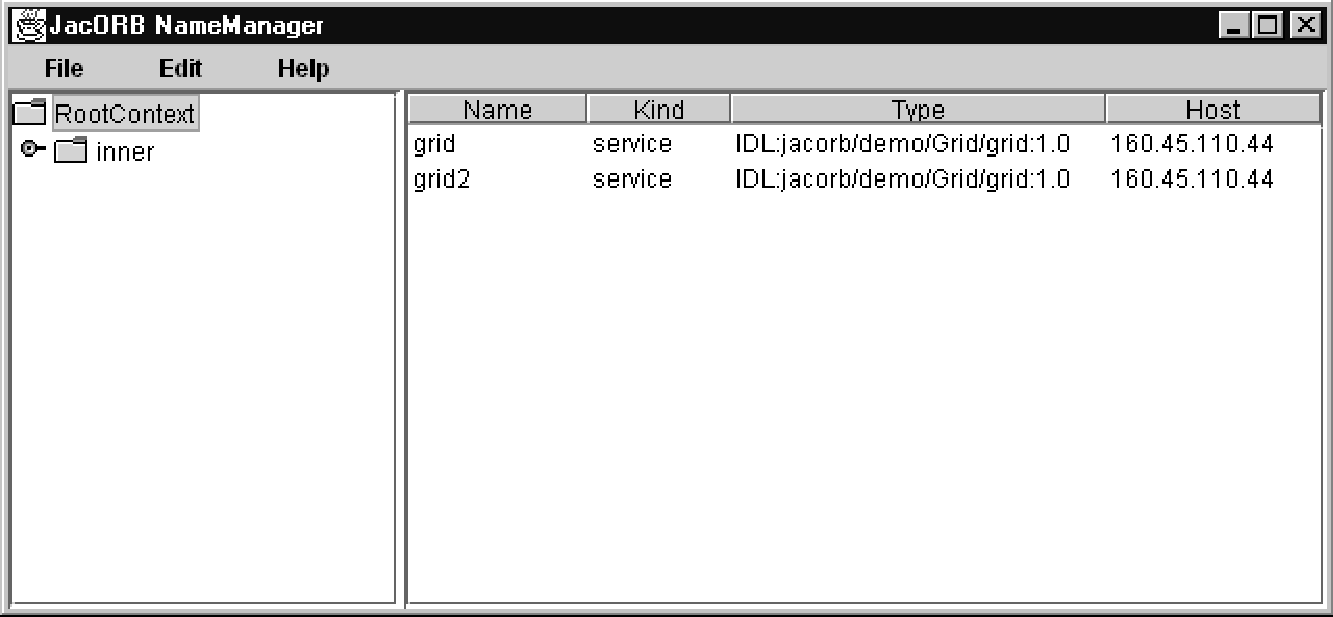
\includegraphics[width=10cm]{Naming/Nmgr1}
  \end{center}
\caption{NameManager Screenshot}
\label{fig:nameManager}
\end{figure}

NameManager has menus that let you bind and unbind names, and create
or delete naming contexts within the root context. Creating a nested
name space, e.g., can be done by selecting the {\tt RootContext} and
bringing up a context by clicking the right mouse button.  After
selecting ``new context'' from that menu, you will be prompted to
enter a name for the new, nested context.


%%% Local Variables: 
%%% mode: latex
%%% TeX-master: "../ProgrammingGuide"
%%% End: 


%%%%%%%%%%%%%%%%%%%%%%%%%%%%%%%%%%%%%%%%%%%%%%%%%%%%%%%%%%%%%%%%%%%%%%%%%%%%%%

\chapter{The server side: POA, Threads}
\label{ch:POA}


This  chapter   describes  the   facilities  offered  by   JacORB  for
controlling  how servers are  started and  executed. These  include an
activation daemon, the Portable Object Adapter (POA), and threading.

This chapter gives only a very superficial introduction to the POA.  A
thorough explanation of how the POA can be used in different settings and of
the different policies and strategies it offers is beyond our scope here, but
can be found in \cite{Brose2001a}.  Other references that explain the POA are
\cite{Henning1999, Vinoski1998}.  More in--depth treatment in C++ can be found
in the various C++-Report Columns on the POA by Doug Schmidt and Steve
Vinoski.  These articles are available at
\href{http://www.cs.wustl.edu/~schmidt/report-doc.html}{http://www.cs.wustl.edu/~schmidt/report-doc.html}.
The ultimate reference, of course, is the CORBA specification.

\section{POA}

The POA provides a comprehensive set of interfaces for managing object
references and servants. The code  written using the POA interfaces is
now portable across ORB implementations  and has the same semantics in
every ORB that is compliant to CORBA 2.2 or above.

The POA defines standard interfaces to do the following:
\begin{itemize}
\item Map an object reference to a servant that implements that object
\item Allow transparent activation of objects
\item Associate policy information with objects
\item  Make a  CORBA  object persistent  over  several server  process
lifetimes
\end{itemize}

In the POA specification, the use of pseudo-IDL has been deprecated in
favor  of an approach  that uses  ordinary IDL,  which is  mapped into
programming languages using the  standard language mappings, but which
is  locality constrained.  This means  that references  to  objects of
these types may not be passed outside of a server's address space. The
POA  interface  itself  is  one  example of  a  locality--constrained
interface.

The  object adapter  is that  part of  CORBA that  is  responsible for
creating CORBA  objects and  object references and  --- with  a little
help  from  skeletons ---  dispatching  operation  requests to  actual
object  implementations.   In  cooperation  with   the  Implementation
Repository  it can also  activate objects,  i.e. start  processes with
programs that provide implementations for CORBA objects.

\section{Threads}

JacORB  currently  offers  one   server--side  thread  model.  The  POA
responsible for a given request will obtain a request processor thread
from  a central  thread pool.  The pool  has a  certain size  which is
always between the maximum and  minimum value configure by setting the
properties     {\tt     jacorb.poa.thread\_pool\_max}     and     {\tt
jacorb.poa.thread\_pool\_min}.

When a  request arrives and  the pool is  found to contain  no threads
because all  existing threads are  active, new threads may  be started
until     the    total    number     of    threads     reaches    {\tt
jacorb.poa.thread\_pool\_max}. Otherwise,  request processing is blocked
until a  thread is returned to  the pool. Upon  returning threads that
have  finished processing a  request to  the pool,  it must  be decided
whether  the  thread  should  actually   remain  in  the  pool  or  be
destroyed. If the current pool  size is above the minimum, a processor
thread will not be returned into the pool again. Thus, the pool size always
oscillates between max and min.

Setting {\tt min} to a value greater than one means keeping a certain number of
threads ready to service incoming requests without delay. As the threadpool can
expand up to the max this is especially useful if you know that requests are
likely to come in in a bursty fashion.  Limiting the pool size to a certain
maximum is done to prevent servers from occupying all available
resources. Setting min to equals max prevents the oscillation in the size of the
pool and the destruction/creation of threads.

Request  processor   threads  usually   run  at  the   highest  thread
priority. It is possible to influence thread priorities by setting the
property  {\tt jacorb.poa.thread\_priority} to  a value  between Java's
Thread.MIN\_PRIORITY and Thread.MAX\_PRIORITY. If the configured priority
value  is  invalid JacORB  will  assign  maximum  priority to  request
processing threads.



%%% Local Variables:
%%% mode: latex
%%% TeX-master: "../ProgrammingGuide"
%%% End:


%%%%%%%%%%%%%%%%%%%%%%%%%%%%%%%%%%%%%%%%%%%%%%%%%%%%%%%%%%%%%%%%%%%%%%%%%%%%%%

\chapter{Implementation Repository}
\label{Ch_Imr}


\begin{quote}
``...  it is  very easy to be blinded to  the essential uselessness of
them by  the sense of achievement you  get from getting it  to work at
all.  In other  words --- and that is a  rock-solid principle on which
the whole of the Corporation's Galaxywide success is founded --- their
fundamental design  flaws are  completely hidden by  their superficial
design flaws.''

             D. Adams: So Long and Thanks for all the Fish
\end{quote}

The Implementation Repository is not, as its name suggests, a database
of  implementations.   Rather,  it  contains information  about  where
requests  to specific  CORBA objects  have  to be  redirected and  how
implementations  can be  transparently  instantiated if,  for a  given
request  to   an  object,  none  is   reachable.   ``Instantiating  an
implementation'' means starting a server program that hosts the target
object.  In  this  chapter  we  give  a brief  overview  and  a  short
introduction  on how to  use the  Implementation Repository.  For more
details please see \cite{Henning1999}.

\section{Overview}

Basically, the  Implementation Repository (ImR) is  an indirection for
requests  using  persistent  object  references. A  persistent  object
reference is one that was created  by a POA with a PERSISTENT lifespan
policy. This means that the lifetime of the object is longer than that
of its creating POA.   Using the Implementation Repository for objects
the lifetime  of which does not exceed  the life time of  its POA does
not make sense  as the main function of  the Implementation Repository
is to take care that such  a process exists when requests are made ---
and to start one if necessary.

To fulfill this function, the ImR  has to be involved in every request
to ``persistent  objects''.  This is achieved  by rewriting persistent
object  references to  contain {\em  not}  the address  of its  server
process but  the address  of the ImR.   Thus, requests  will initially
reach the ImR and not the actual server --- which may not exist at the
time of the request. If such a request arrives at the ImR, it looks up
the  server information  in its  internal tables  to determine  if the
target object is reachable or not.  In the latter case, the ImR has to
have  information  about how  an  appropriate  server  process can  be
started.   After   starting  this   server,  the  client   receives  a
LOCATION\_FORWARD  exception  from  the  ImR.  This  exception,  which
contains a new  object reference to the actual  server process now, is
handled by its runtime system  transparently.  As a result, the client
will automatically  reissue its request  using the new  reference, now
addressing the target directly.

Beside the traditional JacORB ImR, the TAO ImR is also available as an
alternative strategy for Implementation Repository in an operational
environment where both TAO and JacORB service implementations co-exist.
In such an environment, the TAO ImR offers an alternative approach to manage
both JacORB and TAO service implementations.  Please consult the chapter
“TAO Implementation Repository” (\ref{Ch_Tao_Imr}) for details about the
TAO Implementation Repository.

\section{Using the JacORB Implementation Repository}

The  JacORB   Implementation  Repository  consists   of  two  separate
components:  a repository  process which  need  only exist  once in  a
domain, and  process startup daemons,  which must be present  on every
host that is  to start processes. Note that none  of this machinery is
necessary for processes that host  objects with a TRANSIENT life time,
such as used by the RootPOA.

First of all, the central repository process (which we will call ImR
in the following) must be started:

\cmdline{imr [-n] [-p <port>] [-i <ior\_file>][-f <file>][-b <file>] [-a]}

The   ImR   is  located   using   the   configuration  property   {\tt
ORBInitRef.ImplementationRepository}.  This property  must be set such
that  a  http  connection  can  be  made and  the  ImR's  IOR  can  be
read. Next, startup  daemons must be created on  selected hosts. To do
this, the following command must is issued on each host:

\cmdline{imr\_ssd}

When a startup  daemon is created, it contacts  the central ImR.

To register  a program such that  the ImR can start  it, the following
command is used (on any machine that can reach the ImR):

\cmdline{imr\_mg add "AServerName" -c "jaco MyServer"}

The {\tt imr\_mg} command is the  generic way of telling the ImR to do
something. It  needs another command  parameter, such as {\tt  add} in
this case. To add a server to the ImR, an {\em implementation name} is
needed. Here, it is {\tt  "AServerName"}.  If the host were the server
should be  restarted is not the  local one, use the  {\tt -h hostname}
option.  Finally, the  ImR needs to know how to  start the server. The
string {\tt "jaco  MyServer"} tells it how. The  format of this string
is simply such  that the server daemon can execute  it (using the Java
API call  {\tt exec()}), i.e.  it  must be intelligible  to the target
host's operating system.   For a Windows machine, this  could, e.g. be
{\tt "start jaco MyServer"} to have the server run in its own terminal
window, under Unix  the same can be achieved with  {\tt "xterm -e jaco
MyServer"}.

The startup  command is a  string that is  passed as the  {\em single}
argument to javas {\tt Runtime.exec()} method, without interpreting it
or adding  anything. Since {\tt  Runtime.exec()} has system--dependent
behaviour, the startup string has to reflect that. While for most unix
systems  it  is  sufficient  to  avoid shell--expansions  like  *  and
\verb+~+,  windows--based  systems  do   not  pass  the  string  to  a
commandline interpreter so a simple {\tt jaco MyServer} will fail even
if it works if directly typed in at the dos prompt. Therefore you have
to  ``wrap'' the  core  startup command  in  a call  to a  commandline
interpreter. On NT the following startup command will do the job: {\tt
cmd /c "jaco MyServer"}.  Please keep in mind that if you use the {\tt
imr\_mg} command  to set the startup  command, you have  to escape the
quotes so they appear inside of the resulting string.

If you don't  intend to have your server  automatically started by the
ImR     you      can     also     set      the     property     ``{\tt
jacorb.imr.allow\_auto\_register}'' or use the  {\tt -a} switch of the
ImR  process. If  this property  is  set, the  ImR will  automatically
create a new  entry for a server on POA activation,  if the server has
not been registered previously. In this case you don't have to use the
ImR Manager to register your server.

For a client program to be  able to issue requests, it needs an object
reference.  Up to  this  point,  we haven't  said  anything about  how
persistent object  references come into  existence. Reference creation
happens as usual, i.e. in the server application one of the respective
operations  on a  POA is  called.  For a  reference to  be created  as
``persistent'',  the POA  must  have been  created  with a  PERSISTENT
lifespan policy. This is done as in the following code snippet:

\small{
\begin{verbatim}
    /* init ORB and root POA */
    orb = org.omg.CORBA.ORB.init(args, props);
    org.omg.PortableServer.POA rootPOA =
        org.omg.PortableServer.POAHelper.narrow(
                        orb.resolve_initial_references("RootPOA"));

    /* create policies  */

    org.omg.CORBA.Policy [] policies = new org.omg.CORBA.Policy[2];
    policies[0] = rootPOA.create_id_assignment_policy(
                                IdAssignmentPolicyValue.USER_ID);
    policies[1] = rootPOA.create_lifespan_policy(
                                LifespanPolicyValue.PERSISTENT);

    /* create POA */

    POA myPOA = rootPOA.create_POA("XYZPOA",
                                rootPOA.the_POAManager(), policies);

    /* activate POAs */
    poa.the_POAManager().activate();

\end{verbatim}
}

(Note that in general the  id assignment policy will be {\tt USER\_ID}
for a POA with persistent object references because this id will often
be a key into  a database where the object state is  stored). If a POA
is created with this lifespan policy and the ORB property ``use\_imr''
is set, the ORB will try to  notify the ImR about this fact so the ImR
knows it doesn't need to start  a new process for requests that target
objects on this  POA.  To set the ORB policy,  simply set the property
{\tt  jacorb.use\_imr=on}.   The   ORB  uses  another  property,  {\tt
jacorb.implname}, as  a parameter for the  notification, i.e.~it tells
the  ImR  that a  process  using this  property's  value  as its  {\em
implementation name} is present. If  the server is registered with the
ImR, this property value has  to match the implementation name that is
used when registering.

The application  can set  these properties on  the command  line using
{\tt java -Djacorb.implname=MyName}, or in the code like this:

\small{
\begin{verbatim}
    /* create and set properties */
    java.util.Properties props = new java.util.Properties();
    props.setProperty("jacorb.use_imr","on");
    props.setProperty("jacorb.implname","MyName");

    /* init ORB  */
    orb = org.omg.CORBA.ORB.init(args, props);
\end{verbatim}
}

There are a few things  you have to consider especially when restoring
object state  at startup time or  saving the state of  your objects on
shutdown. It is important that, at startup time, object initialization
is complete when the object  is activated because from this instant on
operation calls  may come  in. The repository  knows about  the server
when the  first POA with  a PERSISTENT lifespan policy  registers, but
does not  forward object  references to clients  before the  object is
actually reachable. (Another, unreliable way to handle this problem is
to  increase the {\tt  jacorb.imr.object\_activation\_sleep} property,
so the repository waits longer for the object to become ready again.)

When the server shuts down,  it is equally important that object state
is saved by the time the last POA in the server goes down because from
this moment  the Implementation Repository regards the  server as down
and will start a new one upon requests.  Thus, a server implementor is
responsible for avoiding reader/writer problems between servers trying
to store and  restore the object state.  (One way of  doing this is to
use POA  managers to set  a POA to  holding while saving state  and to
inactive when done.)

Please keep in mind  that even if you don't have to  save the state of
your objects  on server shutdown  you {\em must} deactivate  your POAs
prior   to   exiting   your    process   (or   at   least   use   {\tt
orb.shutdown(\dots)} which  includes POA deactivation).  Otherwise the
ImR keeps the  server as active and will return  invalid IORs. In case
of  a  server crash  you  can either notify the ImR manually by  using
the  command  {\tt imr\_mg  setdown AServerName} or allow the ImR to
detect the crashed server and restart it if necessary.

\section{Server migration}

The  implementation  repository  offers  another  useful  possibility:
server migration.   Imagine the  following scenario: You  have written
your  server with  persistent  POAs,  but after  a  certain time  your
machine  seems   to  be   too  slow  to   serve  all   those  incoming
requests.  Migrating your  server to  a more  powerful machine  is the
obvious  solution.    Using  the  implementation   repository,  client
references do not contain addressing information for the slow machine,
so server migration can be done transparently to client.

Assuming  that you  added your  server to  the repository,  and  it is
running  correctly.

\cmdline{imr\_mg add AServerName -h a\_slow\_machine -c "jaco MyServer"}

The first step is to {\em  hold} the server, that means the repository
delays all requests for that server until it is released again.

\cmdline{imr\_mg hold AServerName}

Now  your server  will not  receive  any requests  for its  registered
POAs. If you can't shut your server down such that it sets itself down
at  the repository,  i.e.~your POAs  are  set to  inactive prior  to
terminating the process, you can use

\cmdline{imr\_mg setdown AServerName}

to  do  that.   Otherwise  your  POAs  can't  be  reactivated  at  the
repository because they are still logged as active.

If you  want your  server to be  restarted automatically, you  have to
tell the repository the new host and maybe a new startup command.

\cmdline{imr\_mg edit AServerName -h the\_fastest\_available\_machine\\
-c "jaco MyServer"}

If your server can be restarted automatically, you now don't even have
to start it manually, but it is instead restarted by the next incoming
request.  Otherwise start it manually on the desired machine now.

The last step is to release  the server, i.e.~let all delayed requests
continue.

\cmdline{imr\_mg release AServerName}

By now your  server should be running on  another machine, without the
clients noticing.

\section{A Note About Security}
Using the imr can pose a major security threat to your system. Imagine
the following standard setup: an imr  is running on a machine, its IOR
file is placed in a directory where  it can be read by the web server,
and several  imr\_ssds are running  on other machines. An  attacker can
now  execute processes  on the  machines the  ssds are  running  on by
taking the following steps:
\begin{enumerate}
         \item  Setting the  {\tt ORBInitRef.ImplementationRepository}
                property to the IOR file on your server.
         \item  Creating a new logical server with the desired command
           to execute as startup command on the desired host (where a
           ssd is running). This is the crucial point. The ssd calls
           {\tt Runtime.exec()} with the supplied string, and there
           is no way to check if the command does what it is supposed
           to do, i.e.~start a server.
         \item Start the server with the imr\_mg. The startup command
           of the server will be exec'd on the specified host.
\end{enumerate}

Now this should  not generally discourage you to use  the imr but show
you  that   there  are  risks,  which  can   be  reduced  significantly
nonetheless. There  are several ways  to encounter this threat  and we
don't consider this list to be complete:
\begin{enumerate}
        \item Try to control the distribution of the IOR file. Hiding
          it should not be considered here, because {\it security by
            obscurity} is generally a bad approach. Try to make use of
          file system mechanisms like groups and ACLs.
          \item Use a firewall which blocks of incoming traffic. Keep
            in mind that if the attacker is inside of your protection
            domain, the firewall won't help. It is also not that hard
            to write a Trojan that can tunnel those firewalls that
            block incoming traffic.
          \item Enforce SSL connections to the imr. This blocks all
            client connections that don't have a certificate signed by
            a CA of your choice. See chapter \ref{ch:SSL} for more
            information.
\end{enumerate}


%%% Local Variables:
%%% mode: latex
%%% TeX-master: "../ProgrammingGuide"
%%% End:


%%%%%%%%%%%%%%%%%%%%%%%%%%%%%%%%%%%%%%%%%%%%%%%%%%%%%%%%%%%%%%%%%%%%%%%%%%%%%%
\chapter{Interface Repository}
\label{ch:interface_repository}

%
% IFR
%

Run--time  type information  in CORBA  is  managed by  the ORB's  {\it
Interface Repository}  (IR) component.  It allows  to request, inspect
and modify IDL  type information dynamically, e.g., to  find out which
operations an object supports. Some ORBs  may also need the IR to find
out whether  a given object's type  is a subtype of  another, but most
ORBs can do  without the IR by encoding this  kind of type information
in the helper classes generated by the IDL compiler.

In essence,  the IR is  just another remotely accessible  CORBA object
that offers  operations to retrieve  (and in theory also  modify) type
information.

\section{Type Information in the IR}

The  IR  manages  type   information  in  a  hierarchical  containment
structure that  corresponds to the structure of  scoping constructs in
IDL  specifications:   modules  contain  definitions   of  interfaces,
structures, constants  etc. Interfaces in turn  contain definitions of
exceptions, operations, attributes  and constants. Figure \ref{IR-fig}
illustrates this hierarchy.

\begin{figure}[htb]
  \begin{center}
    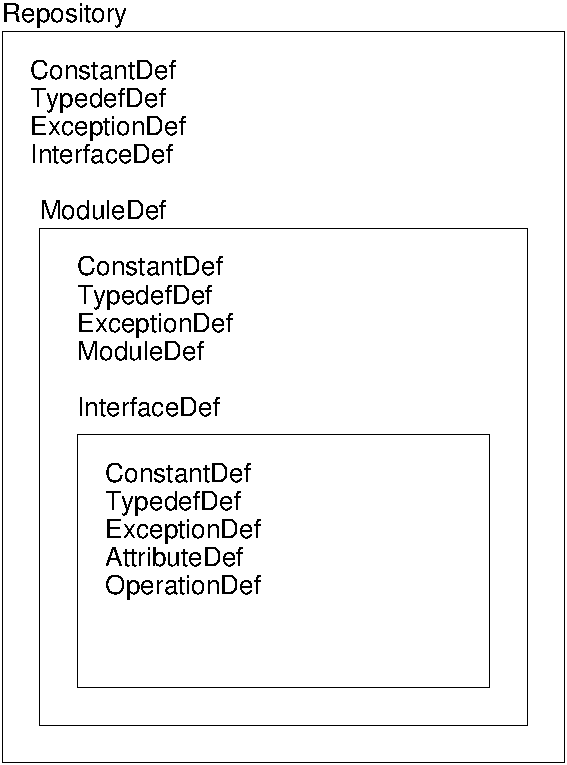
\includegraphics[width=5cm]{IFR/IR}
  \end{center}
\caption{Containers in the Interface Repository}
\label{IR-fig}
\end{figure}

The  descriptions  inside  the  IR  can  be  identified  in  different
ways. Every  element of  the repository has  a unique,  qualified name
which  corresponds  to  the  structure  of  name  scopes  in  the  IDL
specification. An interface {\tt  I1} which was declared inside module
{\tt M2} which in turn was  declared inside module {\tt M1} thus has a
qualified name  {\tt M1::M2::I1}. The  IR also provides  another, much
more   flexible   way   of    naming   IDL   constructs   using   {\it
Repository Id}s.  There   are  a   number  of  different   formats  for
RepositoryIds  but  every  Repository  must  be  able  to  handle  the
following format, which is marked  by the prefix {\tt "IDL:"} and also
carries  a  suffix   with  a  version  number,  as   in,  e.g.,  "{\tt
IDL:jacorb/demo/grid:1.0}". The name  component between the colons can
be set freely using the  IDL compiler directives {\tt \#pragma prefix}
and {\tt \#pragma ID}. If no such directive is used, it corresponds to
the qualified name as above.

\section{Repository Design}

When designing the  Interface Repository, our goal was  to exploit the
Java reflection  API's functionality to  avoid having to  implement an
additional data base for  IDL type descriptions. An alternative design
is to use the IR as a back-end to the IDL compiler, but we did not want
to  introduce such  a  dependency and  preferred  to a  have a  rather
``light--weight'' repository  server.  As  it turned out,  this design
was  possible because  the similarities  between the  Java  and CORBA
object models allow  us to derive the required  IDL information at run
time. As  a consequence,  we can  even do without  any IDL  at compile
time.  In addition  to this simplification, the main  advantage of our
approach lies in avoiding  redundant data and possible inconsistencies
between  persistent IDL descriptions  and their  Java representations,
because Java classes have to be generated and stored anyway.

Thus, the  Repository has to  load Java classes, interpret  them using
reflection  and   translate  them   into  the  appropriate   IDL  meta
information. To  this end, the  repository realizes a  reverse mapping
from   Java   to  IDL.   Figure   \ref{IR-Process}  illustrates   this
functionality,  where $f^{-1}$  denotes  the reverse  mapping, or  the
inverse of  the language  mapping.

\begin{figure}[htb]
  \begin{center}
    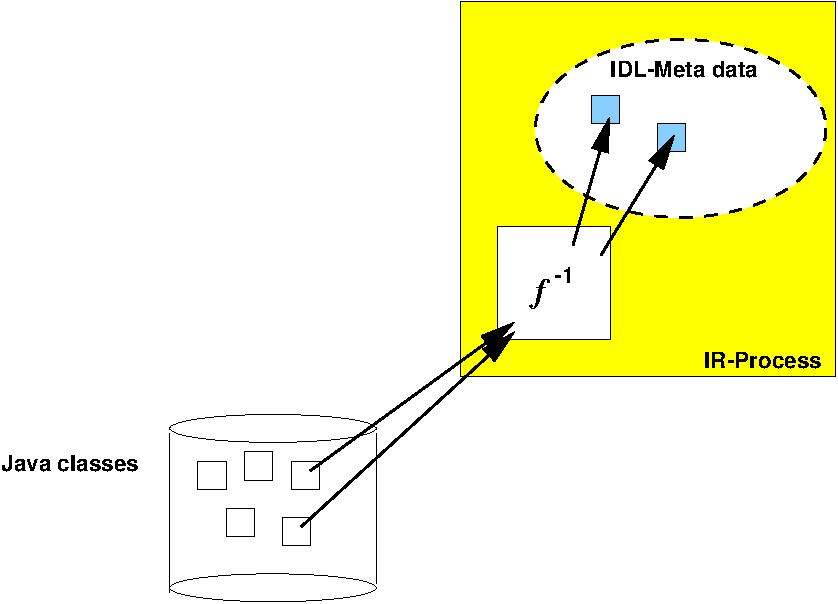
\includegraphics[width=7cm]{IFR/IR-Process}
\end{center}
\caption{The JacORB Interface Repository}
\label{IR-Process}
\end{figure}

\section{Using the IR}

For the ORB to be able to contact the IR, the IR server process must
be running. To start it, simply type the {\tt ir} command and provide
the required arguments:

\cmdline{ir /home/brose/classes /home/brose/public\_html/IR\_Ref}

The first  argument is  a path to  a directory containing  {\tt .class}
files and packages. The IR  loads these classes and tries to interpret
them as  IDL compiler--generated classes.  If it  succeeds, it creates
internal representations  of the  adequate IDL constructs. See below for
instructions on generating classes with IR information. The second
argument on  the command  line above  is simply the  name of  the file
where the IR stores its object reference for ORB bootstrapping.

To view the contents of the repository, you can use the GUI IRBrowser
tool or the query command. First, let's query the IR for a particular
repository ID. JacORB provides the command {\tt qir} (``query IR'')
for this purpose:

\cmdline{qir IDL:raccoon/test/cyberchair/Paper:1.0}

As result, the IR returns an InterfaceDef object, and {\tt qir} parses
this and prints out:

\begin{verbatim}
     interface Paper
     {
        void read(out string arg_0);
        raccoon::test::cyberchair::Review getReview(in long arg_0);
        raccoon::test::cyberchair::Review submitReview(
            in string arg_0, in long a rg_1);
        void listReviews(out string arg_0);
     };
\end{verbatim}

To start the IRBrowser, simply type

\cmdline{irbrowser [ -i <IOR-string> | -f <filename>]}

e.g.

\cmdline{irbrowser}

Note that if no arguments are supplied it will default to using
resolve\_initial\_references.

Figure \ref{fig:IRBrowser} gives a screen shot of the IR browser.

\bigskip
\begin{figure}[htb]
  \begin{center}
    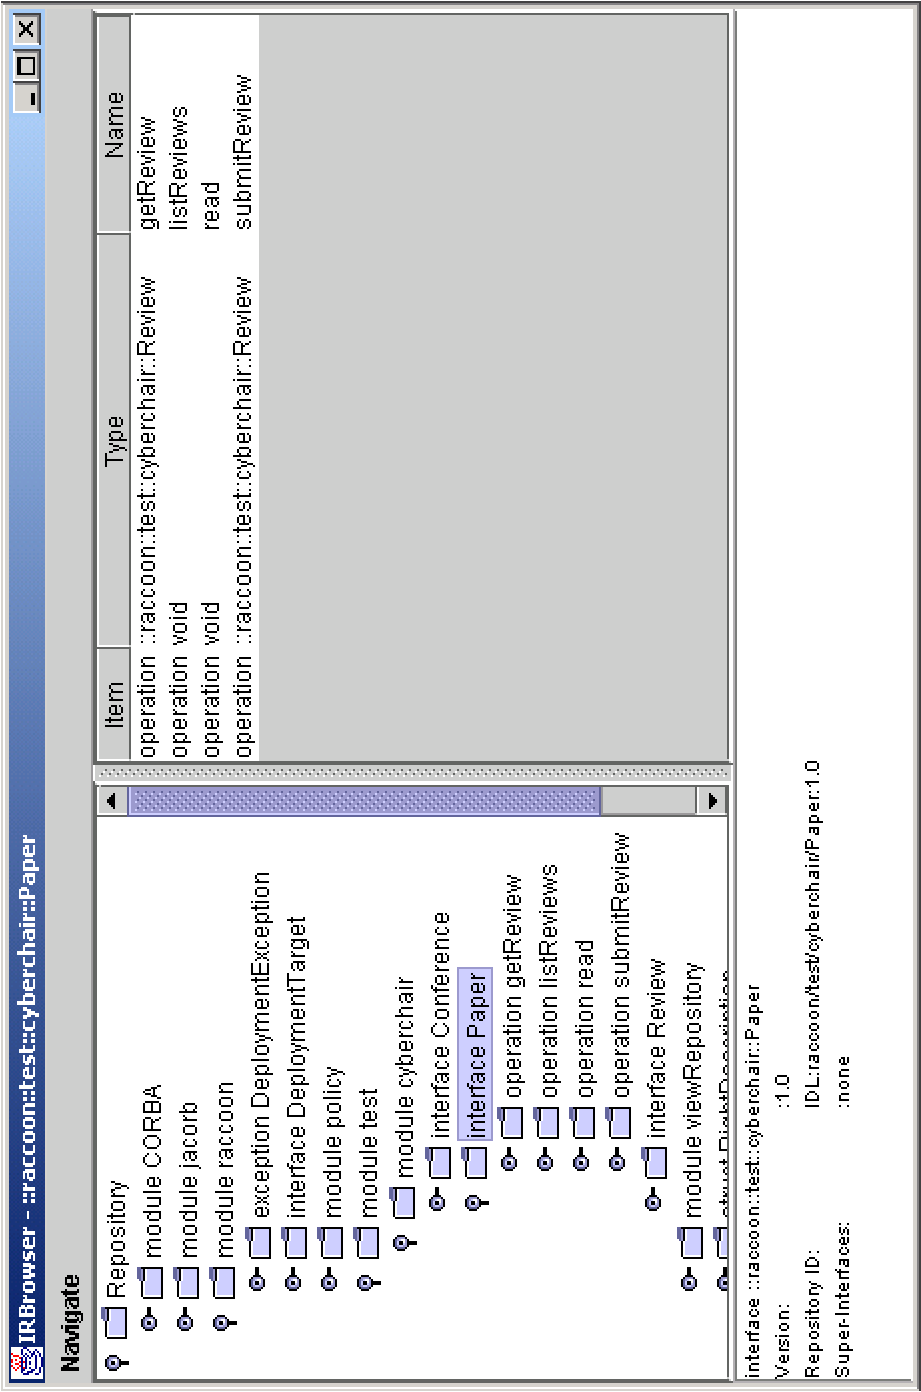
\includegraphics[width=11cm]{IFR/IRBrowser}
\end{center}
\caption{IRBrowser Screenshot}
\label{fig:IRBrowser}
\end{figure}

The Java classes generated by  the IDL compiler using the standard OMG
IDL/Java language mapping do not contain enough information to rebuild
all  of the  information contained  in  the original  IDL file.   For
example,  determining whether an  attribute in  an interface  was {\tt
readonly} or  not is not  possible, or telling the  difference between
{\tt  in}  and {\tt  inout}  parameter  passing  modes. Moreover,  IDL
modules are not  explicitly represented in Java, so  telling whether a
directory in  the class  path represents an  IDL module is  not easily
possible. For these  reasons, the JacORB IDL compiler  generates a few
additional  classes that hold  the required  extra information  if the
compiler switch {\tt -ir} is used when compiling IDL files:

\cmdline{idl -ir myIdlFile.idl}

The additional files generated by the compiler are:
\begin{itemize}
\item a {\tt \_XModule.java} class file for any IDL module X
\item a {\tt YIRHelper.java} class file for any interface Y.
\end{itemize}

\textbf{If no {\tt .class} files that  are compiled from  these extra
classes are found  in the class path passed  to the IR server  process,
the IR will not  be able  to derive any  representations.}
Note that  the IDL compiler does not make any non--compliant modifications
to any of the standard files that are defined in the Java language mapping
 --- there is only additional information.

One more caveat about these  extra classes: The compiler generates the
{\tt  \_XModule.java} class  only  for genuine  modules. Java  package
scopes created by applying the {\tt -d } switch to the IDL compiler do
not  represent   proper  modules  and   thus  do  not   generate  this
class. Thus, the contents of  these directories will not be considered
by the IR.

When an  object's client  calls the {\tt  get\_interface()} operation,
the ORB consults the IR  and returns an {\tt InterfaceDef} object that
describes the object's  interface. Using {\tt InterfaceDef} operations
on  this  description  object,  further  description  objects  can  be
obtained,  such as descriptions  for operations  or attributes  of the
interface under consideration.

The IR  can also be  called like any  other CORBA object  and provides
{\tt lookup()}  or {\tt lookup\_name()} operations to  clients so that
definitions can be searched for, given a qualified name. Moreover, the
complete contents of individual containers (modules or interfaces) can
be listed.

Interface   Repository  meta   objects  provide   further  description
operations. For a given {\tt  InterfaceDef} object, we can inspect the
different  meta   objects  contained   in  this  object   (e.g.,  {\tt
OperationDef} objects). It is  also possible to obtain descriptions in
form of a simple structure  of type {\tt InterfaceDescription} or {\tt
FullInterfaceDescription}. Since structures are  passed by value and a
{\tt   FullInterfaceDescription}    fully   provides   all   contained
descriptions,  no  further  ---possibly  remote  ---  invocations  are
necessary for searching the structure.

\section{Interaction between \#pragma prefix and -i2jpackage}
\label{sec:ifr_pragma_i2jpackage}

Generally any use of \emph{\#pragma prefix} or \emph{-i2jpackage} should be avoided.
if you intend to use a IDL file with the Interface Repository.
If there is no other option there is a property that allows you to
circumvent that restriction in some cases.
Note however that this is a non-standard extension.

If, for example you have the following IDL file:
\begin{verbatim}
    #pragma prefix "org.jacorb.test"

    module ir
    {
        typedef string StringAlias;
        typedef sequence<StringAlias> StringAliasList;

        struct TestStruct
        {
            StringAliasList stringList;
        };
    };
\end{verbatim}

As you want your generated java files to reside in the package \emph{org.jacorb.test.ir} you
need to add \emph{-i2jpackage} as an argument to the \emph{idl} command.
\cmdline{idl -ir -i2jpackage ir:org.jacorb.test.ir myIdlFile.idl}
Now the generated files are in the directory org/jacorb/test/ir.

As the IR starts it reads in the generated classes and implicitely creates
their Repository ID's solely based on the directory structure.
e.g. the struct TestStruct will get the Repository ID {\tt IDL:org/jacorb/test/ir/TestStruct:1.0}
however the correct Repository ID is {\tt IDL:org.jacorb.test/ir/TestStruct:1.0}.

This will make it impossible for you to lookup the correct Repository ID successfully.
starting of the IR will fail if the IR itself needs to look up a Repository ID during start.

As a workaround you can specify the property \emph{jacorb.ir.patch\_pragma\_prefix=on} to the IR server.
this property will cause the IR to change the first component of a requested Repository ID (Repository ID's
consists of multiple components delimited with '/' so its org.jacorb.test in this case).
If the first component looks like a pragma prefix (contains multiple '.') the '.' will be changed to '/'.

So the incoming request for {\tt IDL:org.jacorb.test/ir/TestStruct:1.0} will be
changed to a request for {\tt IDL:org/jacorb/test/ir/TestStruct:1.0} so that the IR will be able to resolve that.

%%% Local Variables:
%%% mode: latex
%%% TeX-master: "../ProgrammingGuide"
%%% End:


%%%%%%%%%%%%%%%%%%%%%%%%%%%%%%%%%%%%%%%%%%%%%%%%%%%%%%%%%%%%%%%%%%%%%%%%%%%%%%

\chapter{Dynamic Management of Any Values}
\label{ch:dynany}

{\em by Jason Courage}

The purpose of this chapter is to describe the DynAny specification,
which is the specification for the dynamic management of Any values.
This chapter only describes the main features of the DynAny
specification; for the complete specification consult the appropriate
chapter of the CORBA specification available from the OMG.

\section{Overview}

DynAny objects are used to dynamically construct and traverse Any
values.  A DynAny can represent a value of a basic type, such as
boolean or long, or a constructed type, such as enum or struct.

\section{Interfaces}

The UML diagram below shows the relationship between the interfaces
in the org.omg.DynamicAny module.

\smallskip
\begin{figure}[htb]
  \begin{center}
    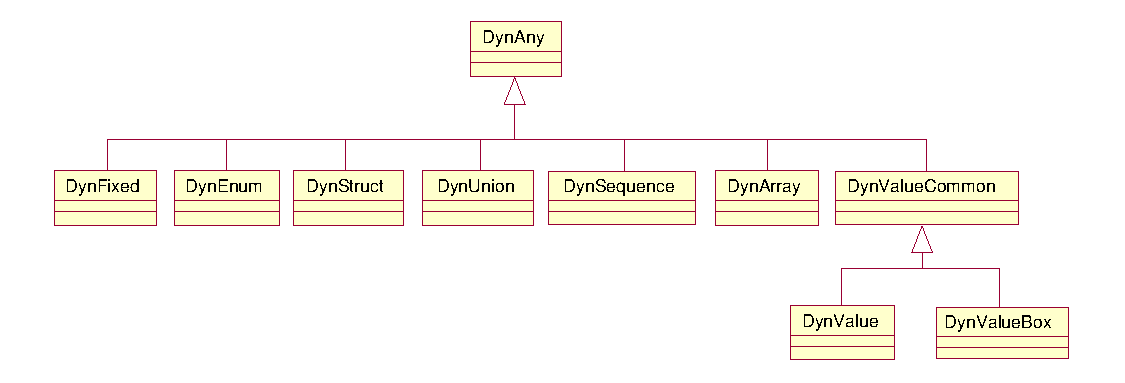
\includegraphics[width=\textwidth]{DynAny/dynany}
  \end{center}
\caption{DynAny Relationships}
\end{figure}


The DynAny interface is the base interface that represents values of
the basic types.  For each constructed type there is a corresponding
interface that extends the DynAny interface and defines operations
specific to the constructed type.  The table below lists the
interfaces in the DynamicAny module and the types they represent.


\begin{small}
\begin{longtable}{|p{6.3cm}|p{8.6cm}|}
\hline
~ \hfill \textbf {Interface} \hfill ~ & ~ \hfill \textbf {Type} \hfill ~ \endhead
\hline
\verb"DynAny" & \verb"basic types (boolean, long, etc.)" \\
\hline
\verb"DynFixed" & \verb"fixed" \\
\hline
\verb"DynEnum" & \verb"enum" \\
\hline
\verb"DynStruct" & \verb"struct" \\
\hline
\verb"DynUnion" & \verb"union" \\
\hline
\verb"DynSequence" & \verb"sequence" \\
\hline
\verb"DynArray" & \verb"array" \\
\hline
\verb"DynValue*" & \verb"non-boxed valuetype" \\
\hline
\verb"DynValueBox*" & \verb"boxed valuetype" \\
\hline

\end{longtable}
\end{small}

* Not currently implemented by JacORB.

\section{Usage Constraints}

Objects that implement interfaces in the DynamicAny module are
intended to be local to the process that constructs and uses them.
As a result, references to these objects cannot be exported to other
processes or externalized using ORB::object\_to\_string;  an
operation that attempts to do so will throw the MARSHAL system
exception.

\section{Creating a DynAny Object}

The DynAnyFactory interface is used to create a DynAny object.  There
are two operations for creating a DynAny object; these are listed in
the table below.


\begin{small}
\begin{longtable}{|p{6.3cm}|p{8.6cm}|}
\hline
~ \hfill \textbf {Operation} \hfill ~ & ~ \hfill \textbf {Description} \hfill ~ \endhead
\hline
\verb"create_dyn_any" & \verb"Constructs a DynAny object from an Any"
\verb"value" \\
\hline
\verb"create_dyn_any_from_ty"
\verb"pe_code" & \verb"Constructs a DynAny object from a"
\verb"TypeCode" \\
\hline

\end{longtable}
\end{small}

The example below illustrates how to obtain a reference to the
DynAnyFacory object and then use it to construct a DynAny object with
each of the create operations.  Exception handling is omitted for
brevity.

The following line of code imports the classes in the DynamicAny
package.

\begin{small}
\begin{verbatim}
import org.omg.DynamicAny.*;

\end{verbatim}
\end{small}

The following code segment obtains a reference to the DynAnyFacory
object.

\begin{small}
\begin{verbatim}
DynAnyFactory factory = null;
DynAny DynAny = null;
DynAny DynAny2 = null;
org.omg.CORBA.Any any = null;
org.omg.CORBA.TypeCode tc = null;
org.omg.CORBA.Object obj = null;

// obtain a reference to the DynAnyFactory
obj = orb.resolve_initial_references ("DynAnyFactory");

// narrow the reference to the correct type
factory = DynAnyFactoryHelper.narrow (obj);

\end{verbatim}
\end{small}

The following code segment creates a DynAny with each of the create
operations.

\begin{small}
\begin{verbatim}
// create a DynAny object from an Any
any = orb.create_any ();
any.insert_long (1);
DynAny = factory.create_dyn_any (any);

// create a DynAny object from a TypeCode
tc = orb.get_primitive_tc (org.omg.CORBA.TCKind.tk_long);
DynAny2 = factory.create_dyn_any_from_type_code (tc);

\end{verbatim}
\end{small}

If the Any value or TypeCode represents a constructed type then the
DynAny can be narrowed to the appropriate subtype, as illustrated
below.

The following IDL defines a struct type.

\begin{small}
\begin{verbatim}
// example struct type
struct StructType
{
   long field1;
   string field2;
};

\end{verbatim}
\end{small}

The following code segment illustrates the creation of a DynStruct
object that represents a value of type StructType.

\begin{small}
\begin{verbatim}
StructType type = null;
DynStruct dynStruct = null;

// create an Any that contains an object of type StructType
type = new StructType (999, "Hello");
any = orb.create_any ();
StructTypeHelper.insert (any, type);

// construct a DynAny from an Any and narrow it to a DynStruct
dynStruct = (DynStruct) factory.create_dyn_any (any);

\end{verbatim}
\end{small}

\section{Accessing the Value of a DynAny Object}

The DynAny interface defines a set of operations for accessing the
value of a basic type represented by a DynAny object.  The operation
to get a value of basic type $<$type$>$ from a DynAny has the form
get\_$<$type$>$.  The operation to insert a value of basic type
$<$type$>$ into a DynAny has the form insert\_$<$type$>$.  A
TypeMismatch exception is thrown if the type of the operation used to
get/insert a value into a DynAny object does not match the type of
the DynAny.

The operations for accessing the value of a constructed type
represented by a DynAny are defined in the interface specific to the
constructed type.  For example, the DynStruct interface defines the
operation get\_members, which returns a sequence of name/value pairs
representing the members of the struct or exception represented by a
DynStruct object.

\section{Traversing the Value of a DynAny Object}

DynAny objects can be viewed as an ordered collection of component
DynAnys.  For example, in a DynStruct object the ordered collection
of component DynAnys is the members of the struct or exception it
represents.  For DynAny objects representing basic types or
constructed types that do not have components, the collection of
component DynAnys is empty.

All DynAny objects have a current position.  For DynAnys representing
constructed types that have components, the current position is the
index of the component DynAny that would be obtained by a call to the
current\_component operation (described in the table below).  The
component DynAnys of a DynAny object are indexed from 0 to n-1, where
n is the number of components.  For DynAnys representing basic types,
or constructed types that do not have components, the current
position is fixed at the value -1.

The operations for traversing the component DynAnys of a DynAny
object are common to all DynAny subtypes, hence they are defined in
the DynAny base interface.  The table below lists the operations
available for traversing a DynAny object.


\begin{small}
\begin{longtable}{|p{6.3cm}|p{8.6cm}|}
\hline
~ \hfill \textbf {Operation} \hfill ~ & ~ \hfill \textbf {Description} \hfill ~ \endhead
\hline
\verb"seek" & \verb"Sets the current position to the"
\verb"specified index" \\
\hline
\verb"rewind" & \verb"Sets the current position to the first"
\verb"component (index 0)" \\
\hline
\verb"next" & \verb"Advances the current position to the"
\verb"next component" \\
\hline
\verb"component_count" & \verb"Returns the number of components" \\
\hline
\verb"current_component" & \verb"Returns the component at the current"
\verb"position" \\
\hline

\end{longtable}
\end{small}

The following code segment illustrates one way of traversing the
component DynAnys of a DynStruct object.  As the DynStruct is
traversed, the value of each component is obtained and printed.
Exception handling is omitted for brevity.

\begin{small}
\begin{verbatim}
DynAny curComp = null;

// print the value of the first component
curComp = dynStruct.current_component ();
System.out.println ("field1 = " + curComp.get_long ());

// advance to the next component
dynStruct.next ();

// print the value of the second component
curComp = dynStruct.current_component ();
System.out.println ("field2 = " + curComp.get_string ());

\end{verbatim}
\end{small}

The next code segment illustrates another way to perform the same
task.

\begin{small}
\begin{verbatim}
// go back to the first component
dynStruct.rewind ();  // same as calling seek (0)

// print the value of the first component
System.out.println ("field1 = " + dynStruct.get_long ());

// advance to the next component
dynStruct.seek (1);

// print the value of the second component
System.out.println ("field2 = " + dynStruct.get_string ());

\end{verbatim}
\end{small}

As the second code segment illustrates, if the component DynAny
represents a basic type, its value can be extracted (or inserted) by
calling the accessor operation on the parent DynAny directly, rather
than first obtaining the component using the current\_component
operation.

\section{Constructed Types}

This section describes the interfaces in the DynamicAny module that
represent the constructed types supported by JacORB.  Each of these
interfaces extends the DynAny interface.



\subsection{DynFixed}

A DynFixed object represents a fixed value.  Since IDL does not have
a generic type to represent a fixed type, the operations in this
interface use the IDL string type.  The value represented by a
DynFixed object can be accessed (as a string) using the get\_value
and set\_value operations.

A DynFixed object has no components.

\subsection{DynEnum}

A DynEnum object represents a single enumerated value.  The integer
(ordinal) value of the enumerated value can be accessed with the
get\_as\_ulong and set\_as\_ulong operations.  The string (IDL
identifier) value of the enumerated value can be accessed with the
get\_as\_string and set\_as\_string operations.

A DynEnum object has no components.

\subsection{DynStruct}

A DynStruct object represents a struct value or an exception value.
The current\_member\_name and current\_member\_kind operations return
the name and TCKind value of the TypeCode of the member at the
current position of the DynStruct.  The members of the DynStruct can
be accessed with the get\_members and set\_members operations.

The component DynAnys of a DynStruct object are the members of the
struct or exception.  A DynStruct representing an empty exception has
no components.

\subsection{DynUnion}

A DynUnion object represents a union value.  The value of the
discriminator can be accessed using the get\_discriminator and
set\_discriminator operations.

If the discriminator is set to a value that names a member of the
union then that member becomes active.  Otherwise, if the value of
the discriminator does not name a member of the union then there is
no active member.

If there is an active member, the member operation returns its value
as a DynAny object, and the member\_name and member\_kind operations
return its name and the TCKind value of its TypeCode.  These
operations throw an InvalidValue exception if the union has no active
member.

A DynUnion object can have either one or two components.  The first
component is always the discriminator value.  The second component is
the value of the active member, if one exists.

\subsection{DynSequence}

A DynSequence object represents a sequence.  The length of the
sequence can be accessed using the get\_length and set\_length
operations.  The elements of the sequence can be accessed using the
get\_elements and set\_elements operations.

The component DynAnys of a DynSequence object are the elements of the
sequence.

\subsection{DynArray}

A DynArray object represents an array.  The elements of the array can
be accessed using the get\_elements and set\_elements operations.

The component DynAnys of a DynArray object are the elements of the
array.

\section{Converting between Any and DynAny Objects}

The DynAny interface defines operations for converting between Any
objects and DynAny objects.  The from\_any operation initialises the
value of a DynAny with the value of a specified Any.  A TypeMismatch
exception is thrown if the type of the Any does not match the type of
the DynAny.  The to\_any operation creates an Any from a DynAny.

As an example of how these operations might be useful, suppose one
wants to dynamically modify the contents of some constructed type,
such as a struct, which is represented as an Any.  The following
steps will accomplish this task:

\begin{enumerate}
  \item  A DynStruct object is constructed from the TypeCode of the struct using the DynAnyFactory::create\_dyn\_any\_from\_type\_code operation.
  \item  The DynAny::from\_any operation is used to initialise the value of the DynStruct with the value of the Any.
  \item  The contents of the DynStruct can now be traversed and modified.
  \item  A new Any can be created to represent the modified struct using the DynAny::to\_any operation.
\end{enumerate}

\section{Further Examples}

The demo/dynany directory of the JacORB repository contains example
code illustrating the use of DynAny objects.  Further code can be
found in the org.jacorb.test.orb.dynany package of the JacORB-Test
repository.


%%% Local Variables: 
%%% mode: latex
%%% TeX-master: "../ProgrammingGuide"
%%% End: 


%%%%%%%%%%%%%%%%%%%%%%%%%%%%%%%%%%%%%%%%%%%%%%%%%%%%%%%%%%%%%%%%%%%%%%%%%%%%%%
\chapter{Objects By Value}
\label{ch:obv}


Until CORBA 2.3, objects could only be passed using reference
semantics: there was no way to specify that object state should be
copied along with an object reference. A further restriction of the
earlier CORBA versions was that all non-object types (structs, unions,
sequences, etc.) were {\em values}, so you could not use, e.g. a
reference-to-struct to construct a graph of structure values that
contained shared nodes. Finally, there was no inheritance between
structs.

All these shortcomings are addressed by the {\em objects-by-value} (OBV)
chapters of the CORBA specification: the addition of stateful
value types supports copy semantics for objects and inheritance for
structs, boxed value types introduce reference semantics for base
types, and abstract interfaces determine whether an argument is sent
by-value or by-reference by the argument's runtime type. The
introduction of OBV into CORBA presented a major shift in the CORBA
philosophy, which had been to strictly avoid any dependence on
implementation details (state, in particular). It also added a
considerable amount of marshaling complexity and interoperability
problems. (As a personal note: Even in CORBA 2.6, the OBV marshaling
sections are still not particularly precise...)

JacORB 2.0 implements most of the OBV specification.  Boxed value
types and regular value types work as prescribed in the standard
(including value type inheritance, recursive value types, and
factories).  Still missing in the current implementation is run-time
support for abstract value types (although the compiler does accept
the corresponding IDL syntax), and the marshaling of truncatable
value types does not yet meet all the standard's requirements (and
should thus be called ``beta'').

\section{Example}

To illustrate the use of various kinds of value types, here's an
example which is also part of the demo programs in the JacORB
distribution.  The demo shows the use of boxed value types and a
recursive stateful value type. Here's the IDL definition from {\tt
demo/value/server.idl}:

\begin{verbatim}
module demo {
  module value {

     valuetype boxedLong   long;
     valuetype boxedString string;

     valuetype Node {
        public long id;
        public Node next;
     };

     interface ValueServer {
        string receive_long   (in boxedLong p1, in boxedLong p2);
        string receive_string (in boxedString s1, in boxedString s2);
        string receive_list   (in Node node);
     };
  };
};
\end{verbatim}

From the definition of the  boxed value type {\tt boxedLong} and
{\tt boxedString}, the IDL generates the following Java class, which
is simply a holder for the long value. No mapped class is generated
for the boxed string value type.

\begin{verbatim}
package demo.value;

public class boxedLong
    implements org.omg.CORBA.portable.ValueBase
{
    public int value;
    private static String[] _ids = { boxedLongHelper.id() };

    public boxedLong(int initial )
    {
        value = initial;
    }
    public String[] _truncatable_ids()
    {
        return _ids;
    }
}
\end{verbatim}

The boxed value definitions in IDL above permit uses of non-object
types that are not possible with IDL primitive types. In particular, it
is possible to pass Java {\tt null} references where a value of a
boxed value type is expected. For example, we can call the operation
{\tt receive\_long} and pass one initialized {\tt boxedLong} value and
a null reference, as show in the following snippet from the client
code:

\begin{verbatim}
    ValueServer s = ValueServerHelper.narrow( obj );
    boxedLong boxL = new boxedLong (774);

    System.out.println ("Passing two integers: "
                       + s.receive_long ( boxL , null ));
\end{verbatim}

With a regular {\tt long} parameter, a {\tt null} reference would have
resulted in a {\tt BAD\_PARAM} exception. With boxed value types, this
usage is entirely legal and the result string returned from the {\tt
  ValueServer} object is {\tt ``one or two null values''}.

A second new possibility of the reference semantics that can be
achieved by ``boxing'' primitive IDL types is {\em sharing} of values.
With primitive values, two variables can have copies of the same
value, but they cannot both refer to the same value. This means that
when one of the variables is changed, the other one retains its
orignal value. With shared values that are {\em referenced}, both
variables would always point to the same value.

The stateful value type {\tt Node} is implemented by the programmer in
a class {\tt NodeImpl} (see the JacORB distribution for the actual
code).  The relationship between this implementation class and the
corresponding IDL definition is not entirely trivial, and we will
discuss it in detail below.

\section{Factories}

When an instance of a (regular) value type is marshaled over the wire
and arrives at a server, a class that implements this value type must
be found, so that a Java object can be created to hold the state
information.  For interface types, which are only passed by
reference, something similar is accomplished by the POA, which
accepts remote calls to the interface and delivers them to a local
implementation class (the \emph{servant}).  For value type instances,
there is no such thing as a POA, because they cannot be called
remotely.  Thus, the ORB needs a different mechanism to know which
Java implementation class corresponds to a given IDL value type.

The CORBA standard introduces \emph{value factories} to achieve this.
Getting your value factories right can be anywhere from trivial to
tricky (we will cover the details in a minute), and so the standard
suggests that ORBs also provide convenience mechanisms to relieve
programmers from writing value factories if possible.  JacORB's
convenience mechanism is straightforward:

\begin{quotation}
\noindent \emph{If the implementation class for an IDL value type A is named
  AImpl, resides in the same package as A, and has a no-argument
constructor, then no value factory is needed for that type.}
\end{quotation}

In other words, if your implementation class follows the common naming
convention (``...Impl''), and it provides a no-arg constructor
so that the ORB can instantiate it, then the ORB has all that it
needs to (a) find the implementation class, and (b) create an instance
of it (which is then initialized with the unmarshaled state from the
wire).

This mechanism ought to save you from having to write a value factory
99\% of the time.  It works for all kinds of regular value types,
including those with inheritance, and recursive types (where a type
has members of its own type).

If you do need more control over the instance creation process, or the
unmarshaling from the wire, you can write your own value factory
class and register it with the ORB using {\tt
ORB.register\_value\_factory(}\emph{repository\_id, factory}{\tt)}.
The \emph{factory} object needs to implement the interface {\tt
org.omg.CORBA.portable.ValueFactory}, which requires a single method:

\begin{verbatim}
   public Serializable read_value (InputStream is);
\end{verbatim}

When an instance of type \emph{repository\_id} arrives over the wire,
the ORB calls the {\tt read\_value()} method, which must unmarshal the
data from the input stream, create an instance of the appropriate
implementation class from it, and return that.

The easiest way to implement this method is to create an instance of
the implementation class, and pass it to the {\tt read\_value()} method
of the given InputStream:

\begin{verbatim}
   public Serializable read_value (InputStream is) {
     A result = new AImpl();
     return is.read_value(result);
   }
\end{verbatim}

The {\tt InputStream.read\_value()} method registers the newly created
instance in the stream's indirection table, and then reads the data
from the stream and initializes the given {\tt value} instance from
it.

The value factory must be registered with the ORB using {\tt
 register\_value\_factory()}.  As a special convenience (defined in
 the CORBA standard), if the value factory class for type {\tt A} is
 called {\tt ADefaultFactory}, then the ORB will find it automatically
 and use it, unless a different factory has been explicitly
 registered.

It sometimes causes confusion that you can also define \emph{factory
methods} in a value type's IDL.  These factory methods are completely
unrelated to the unmarshaling mechanism discussed above; they are
simply a portable means to declare what kinds of ``constructors'' a
value type implementation should have.  They are purely for local use,
but since they are ``factories'', the corresponding methods must also
be implemented in the type's {\tt ValueFactory} implementation.


%%% Local Variables: 
%%% mode: latex
%%% TeX-master: "../ProgrammingGuide"
%%% End: 


%%%%%%%%%%%%%%%%%%%%%%%%%%%%%%%%%%%%%%%%%%%%%%%%%%%%%%%%%%%%%%%%%%%%%%%%%%%%%%

\chapter{IIOP over SSL}
\label{ch:SSL}



Using  SSL to authenticate  clients and  to protect  the communication
between client and target requires no changes in your source code. The
only  notable  effect  is  that  SSL/TLS type  sockets  are  used  for
transport  connections  instead of  plain  TCP  sockets  --- and  that
connection setup takes a bit longer.

The only  prerequisites are that you rebuild  JacORB with cryptography
support. You  also need  to set up  a key  store file that  holds your
cryptographic   keys,  and  to   configure  SSL   by  setting   a  few
properties. All of this is described in this chapter.

\section{Re--Building JacORB's security libraries}

In the  standard distribution, the  JacORB security libraries  are not
enabled.   To do  so, you  simply need  to recompile  JacORB  with the
required SSL libraries  in your CLASSPATH.  If these libraries
are not found, JacORB will be rebuilt without SSL support.

To  successfully rebuild  JacORB with  SSL support,  the  following is
required:

\begin{itemize}
        \item when using IAIKs libraries:
              \begin{itemize}
                \item IAIK-JCE 2.591 or later, the security provider classes
                downloadable from \\ \href{http://jcewww.iaik.tu-graz.ac.at}{http://jcewww.iaik.tu-graz.ac.at},
              \item iSaSiLk 3.0 or later, the SSL implementation from the same
                source.
              \end{itemize}

        \item when using Suns libraries:
              \begin{itemize}
              \item JDK 1.4 or jsse1.0.2 available from the Developer
                Connection (for jsse1.0.2, please see the {\tt README.jsse\_1\_0\_2} in
                {\tt src/org/jacorb/security/ssl/sun\_jsse} on how to compile).
              \item For key management, you also need additional packages like
                OpenSSL. These are not necessary for JacORB to work.
              \end{itemize}
\end{itemize}

Install the desired packages and read the documentation carefully. After
successfull installation, build JacORB anew by typing {\tt ant} in your JacORB
installation directory.


\section{IAIK specific setup}
This section covers topics that are specific to IAIKs libraries.

\subsection{Setting up an IAIK key store}

SSL  relies   on  public  key  certificates  in   the  standard  X.509
format. These  certificates are presented in  the authentication phase
of the  SSL handshake and used  to compute and  exchange session keys.
This section explains how to create and store these certificates.

The Java 2  security API provides interfaces that  access a persistent
data structure  called {\em  KeyStore}. A key  store is simply  a file
that contains  public key  certificates and the  corresponding private
keys. It also  contains other certificates that can  be used to verify
public key  certificates.  All  cryptographic data is  protected using
passwords and accessed using names called {\em aliases}.

JacORB provides a  GUI tool to create and  manipulate key store files,
the  KeyStoreManager. It  can generate  key pairs,  sign  public keys,
import  or   export  certificates,  and   define  trusted  certificate
authorities. To start the KeyStoreManager, simply type {\tt ks} on the
command  line. The GUI  lets you  select and  open existing  key store
files, or create new ones.

Starting with an  empty key store, you first need to  create a new key
store and then  a key pair and certificate. Select  {\tt New} from the
{\tt File}  menu to create  a key store,  and then {\tt New}  from the
{\tt Keys} menu.   You will then be asked to provide  a new alias name
for your  new key entry. You also  need to choose a  password. You can
leave  the  algorithm  and  key  length fields  in  the  combobox  menu
unchanged.

\bigskip
\begin{center}
  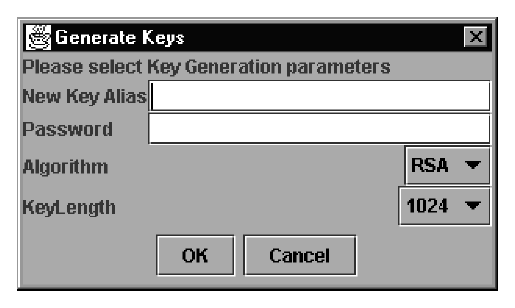
\includegraphics[width=7cm]{SSL/Generate}
\end{center}

You  now  have a  public  key certificate  that  you  can present  for
authentication, claiming  identity with the  alias name that  has been
embedded  in the  certificate.   Since anybody  could  present such  a
certificate,  receivers  require  that  the certificate  be  digitally
signed by someone  they trust, a {\em Certificate  Authority} (CA). By
signing  the certificate,  a CA  supports  the identity  claim of  the
certificate  subject. Whose  signature is  accepted as  trustworthy is
just a matter  of configuration, but normally proper  CAs are expected
to only sign certificates that  they have carefully scrutinized --- or
even created themselves.

\bigskip
\centerline{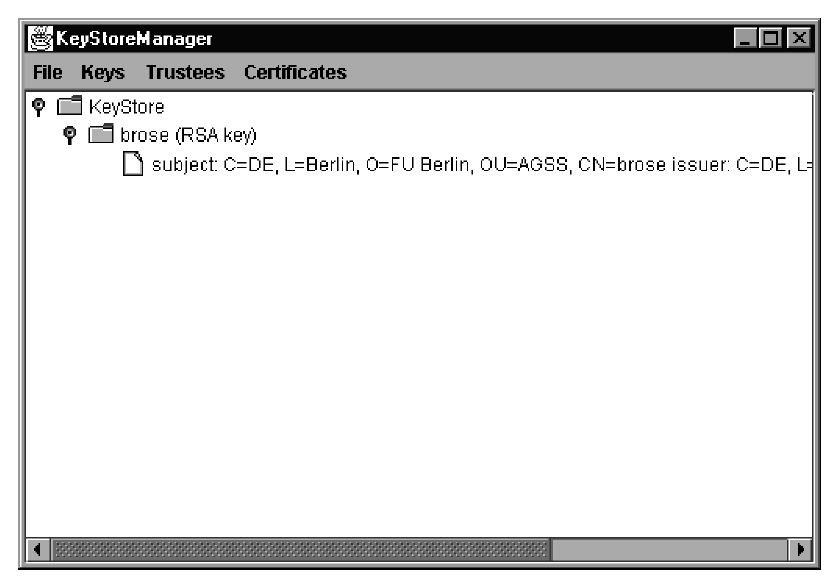
\includegraphics[width=11cm]{SSL/Keystore}}

For   convenience  you   can  act   as  a   CA  yourself,   using  the
KeyStoreManager GUI  to import certificates  and then sign  and export
them  again.   The  originating  key  store can  then  re--import  the
certificate that now bears the  digital signature of someone acting as
a CA. The key store has a  standard key chain format that must be used
to store public key certificates. The  first entry in the key chain is
your own public  key certificate as generated by the  key store. It is
automatically signed with its own  private key. Second in the chain is
the public key certificate that is signed by the CA. The last entry in
a key  chain must hold the  CA's public key  certificate, signed using
its private key. Trust in the CA key is ``axiomatic''.

\bigskip
\centerline{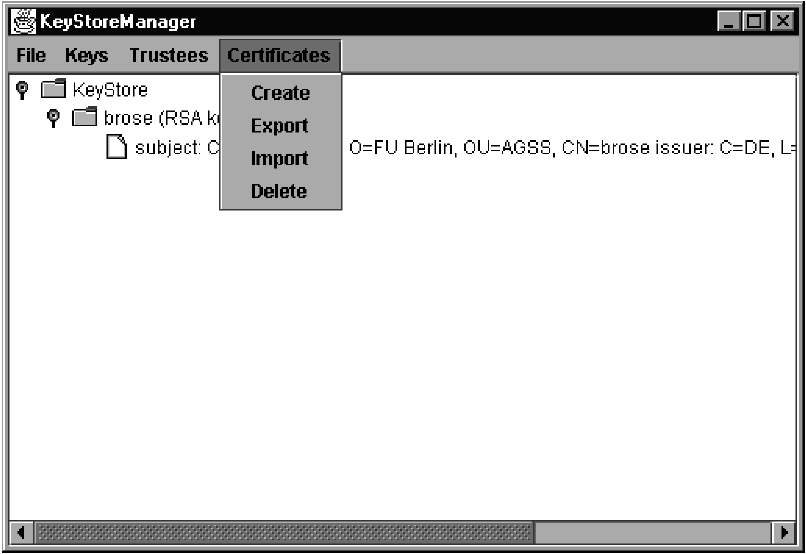
\includegraphics[width=11cm]{SSL/KSMenu}}

You can  check the validity of a  key chain by selecting  an alias and
then choosing {\tt Verify Chain}  from the {\tt Keys} menu. Unless the
key  chain  has  the proper  format  {\em  and}  the CA's  public  key
certificate is also declared  as trusted using the {\tt Trustees--add}
menu, the  verification will fail.  Only of  the verification succeeds
will you be able to use a public key certificate in the SSL connection
setup. More documentation on key stores  can be found in the Java tool
documentation for the {\tt keytool}  command. If you care for ``real''
security,  be advised  that setting  up  and managing  (or finding)  a
properly administered CA is essential for the overall security of your
system.

Finally,  note that  key  stores  are normally  used  only for  client
authentication in JacORB.   Servers may, but need not,  have their own
keys and  passwords because server authentication is  optional and not
mandatory like  client authentication. Technically,  this is achieved
by  exchanging the  client  and server  roles  at SSL  setup. This  is
entirely  transparent to  applications, of  course, but  might prevent
interoperation  with other ORBs  over SSL  if their  SSL setup  is not
prepared to handle this role change.

\subsection{Step--By--Step certificate creation}
In  order to  generate  a  simple public  key  infrastructure you  can
perform the following steps:
\begin{enumerate}
\item Create new keystores (File/new) and keypairs (Keys/new) for the CA
and for the user.
\item  Open the  user keystore (File/open),  select the  key  entry and
export the self-signed certificate (Certificates/Export).
\item  Open  the  CA  keystore  and  add the  user  certificate  as  a
Trustee (Trustees/add\dots).
\item Select the  trusted user certificate and create  a signed public
key certificate (Certificates/Create). Leave the role name field empty,
enter the  CAs private  key password and  save the new  certificate by
clicking OK.
\item Export the  CAs self-signed certificate to a  file (as explained
above).    Delete    the    trusted    certificate   from    the    CA
keystore (Trustees/Delete).
\item Open the  user keystore again. Select the  key entry, the import
the CA-signed  user cert (Certificates/Import), and  the self-signed CA
cert.
\item Add  the self-signed CA cert  as a trustee. This  is only needed
for verifying the chain, therefor the keystore can be deployed without
it.  Please  note  that  a  failed  verification  might  result  in  a
SignatureException.
\end{enumerate}

\section{Configuring SSL properties}

When the ORB is initialized by the application, a couple of properties
are read from files and the  command line. To turn on SSL support, you have to
set the following property to ``on'':

\begin{verbatim}
        jacorb.security.support_ssl=on
\end{verbatim}

This will just load the SSL classes on startup. The configuration of the
various aspects of SSL is done via additional properties.

As explained  in the previous  section, cryptographic data  (key pairs
and  certificates) is  stored in  a  keystore  file. To configure the
file name of the keystore file, you need to define the following
property:

\begin{verbatim}
        jacorb.security.keystore=AKeystoreFileName
\end{verbatim}

The keystore file name can either be an absolute path or relative to
the home directory. Keystores are searched in this order, and the
first one found is taken. If this property is not set, the user will be
prompted to enter a keystore location on ORB startup.

To avoid  typing in  lots of  aliases and passwords  (one for  the key
store, and  one for each entry  that is used), you  can define default
aliases and passwords like this:

\begin{verbatim}
# the name of the default key alias to look up in the keystore
jacorb.security.default_user=brose
jacorb.security.default_password=jacorb
\end{verbatim}


These SSL settings can be further refined using security options as in
the following property definitions:

\begin{verbatim}
        jacorb.security.ssl.client.supported_options=0
        jacorb.security.ssl.client.required_options=0

        jacorb.security.ssl.server.supported_options=0
        jacorb.security.ssl.server.required_options=0
\end{verbatim}

The  value  of  these security  options  is  a  bit  mask coded  as  a
hexadecimal integer. The meanings of the individual bits is defined in
the CORBA Security Service  Specification and reproduced here from the
{\tt Security.idl} file:

\begin{verbatim}
        typedef unsigned short   AssociationOptions;

        const AssociationOptions NoProtection = 1;
        const AssociationOptions Integrity = 2;
        const AssociationOptions Confidentiality = 4;
        const AssociationOptions DetectReplay = 8;
        const AssociationOptions DetectMisordering = 16;
        const AssociationOptions EstablishTrustInTarget = 32;
        const AssociationOptions EstablishTrustInClient = 64;
        const AssociationOptions NoDelegation = 128;
        const AssociationOptions SimpleDelegation = 256;
        const AssociationOptions CompositeDelegation = 512;
\end{verbatim}

% With the current SSL integration in JacORB, the only valid settings
% are EstablishTrustInTarget and/or EstablishTrustInClient, i.e.  hex
% values 20, 40 or 60. NoProtection is not possible when SSL is used. If
% you don't want protection, switch SSL support off. The following
% sections go into some more detail about what specific property values
% mean.

\subsection{Client side configuration}

\begin{verbatim}
   jacorb.security.ssl.client.supported_options=20 //EstablishTrustInTarget
\end{verbatim}
This value indicates that the client can use SSL. Actually, this is default
SSL behaviour and must always be supported by the client.

\begin{verbatim}
   jacorb.security.ssl.client.supported_options=40 //EstablishTrustInClient
\end{verbatim}
This makes the client load it's own key/certificate from it's
keystore, because it must be prepared to authenticate to the server.

\begin{verbatim}
   jacorb.security.ssl.client.required_options=20 //EstablishTrustInTarget
\end{verbatim}
This enforces SSL to be used.

\begin{verbatim}
   jacorb.security.ssl.client.required_options=40 //EstablishTrustInClient
\end{verbatim}
This enforces SSL to be used. Actually, this is no meaningfuly value, since in
SSL, the client can't force it's own authentication to the server.


\subsection{Server side configuration}

\begin{verbatim}
   jacorb.security.ssl.server.supported_options=1 //NoProtection
\end{verbatim}
This tells the clients that the server also supports unprotected
connections. If NoProtection is set, no required options should be set as
well, because they override this value.

\begin{verbatim}
   jacorb.security.ssl.server.supported_options=20 //EstablishTrustInTarget
\end{verbatim}
This value indicates that the server supports SSL. Actually, this is default
SSL behaviour and must always be supported by the server. This also makes the
server load it's key/certificate from the keystore.

\begin{verbatim}
   jacorb.security.ssl.server.supported_options=40 //EstablishTrustInClient
\end{verbatim}
This value is ignored, because authenticating the client is either
required, or not done at all (the client can't force its own
authentication).

\begin{verbatim}
   jacorb.security.ssl.server.required_options=20 //EstablishTrustInTarget
\end{verbatim}
This enforces SSL to be used.

\begin{verbatim}
   jacorb.security.ssl.server.required_options=40 //EstablishTrustInClient
\end{verbatim}
This enforces SSL to be used, and will request the client to authenticate. It
also will load trusted certificates for the authentication process.



%%% Local Variables: 
%%% mode: latex
%%% TeX-master: "../ProgrammingGuide"
%%% End: 


%%%%%%%%%%%%%%%%%%%%%%%%%%%%%%%%%%%%%%%%%%%%%%%%%%%%%%%%%%%%%%%%%%%%%%%%%%%%%%

\chapter{MIOP}
\label{ch:miop}

%
% Contents???
% Properties
% Corbaloc
% Demo example


JacORB has an implementation of MIOP written as an ETF plugin. This
conforms to version 01-11-08 of the Unreliable Multicast Inter-ORB
Protocol specification.


\section{Enabling the MIOP Transport}
In order to enable the ETF transport plugin the following configuration
properties must be altered.
\begin{verbatim}
jacorb.transport.factories
jacorb.transport.client.selector
\end{verbatim}
By default these properties are configured to use the IIOP transport. For example
to select both IIOP and MIOP transports:
\begin{verbatim}
jacorb.transport.factories=org.jacorb.orb.iiop.IIOPFactories,
                           org.jacorb.orb.miop.MIOPFactories
jacorb.transport.client.selector=
                           org.jacorb.orb.miop.MIOPProfileSelector
\end{verbatim}


\section{Configuring the MIOP Transport}
\label{miopConfig}
A number of extra configuration properties have been added for the transport.



\begin{small}
\begin{longtable}{|p{5cm}|p{9cm}|p{2cm}|}
\caption{MIOP Configuration}\\
\hline
~ \hfill \textbf {Property} \hfill ~ & ~ \hfill \textbf {Description} \hfill ~ & ~ \hfill \textbf {Type} \hfill ~ \endhead
\hline
\verb"jacorb.miop.timeout" & Timeout used in MIOP requests. Default is 100. &
 integer \\
\hline
\verb"jacorb.miop.time_to_"
\verb"live" & TTL used for multicast UDP packets. Default
is 5 seconds. & integer \\
\hline
\verb"jacorb.miop.incomplete_"
\verb"messages_threshold" & Maximum number of incomplete messages allowed.
Default 5. & integer \\
\hline
\verb"jacorb.miop.message_"
\verb"completion_timeout" & Timeout for packet collection to be completed.
Default 500ms. & integer \\
\hline
\verb"jacorb.miop.packet_"
\verb"max_size" & This is the maximum size of the frame buffer. This defaults
to 1500 bytes which is the typical value for most network interfaces. From this
the IP, UDP and UMIOP headers will be deducted which will leave 1412 bytes for
the MIOP packet. & integer \\
\hline
\end{longtable}
\end{small}



\section{MIOP Example}

A new demo has been included within {\tt <JacORB>/demo/miop}. This section will
describe how to run this demo including its use of MIOP corbaloc strings.

Assuming the developer has installed Ant {\small version 1.7.1} or above then
the example may be compiled by typing {\tt ant} within the {\tt <JacORB>/demo/miop}
directory. The classes will be compiled to {\tt <JacORB>/classes} which may
need to be added to the classpath.


To run the server:
\begin{small}
\begin{verbatim}
jaco demo.miop.Server
\end{verbatim}
\end{small}

To run the client:
\begin{small}
\begin{verbatim}
jaco demo.miop.Client
\end{verbatim}
\end{small}

This is the simplest configuration and will simply send two oneway requests via
UDP to the server. By default the Server will write out a miop.ior file
containing the following corbaloc:

\begin{verbatim}
corbaloc:miop:1.0@1.0-TestDomain-1/224.1.239.2:1234;
         iiop:1.2@10.1.0.4:38148/4222541922/%00%16%0F%205=%25%02%01I%0C
\end{verbatim}
The Group IIOP Profile key string will not remain constant. The server takes a
single optional argument:
\begin{tabbing}
XX \= XXXXXXXXXXXXX \= XX \kill
\>  -noGroupProfile \>  Don't write IIOP Group Profile
request.\\
\end{tabbing}
This will create a corbaloc as shown below and is useful for interoperating
with ORBs that do not support the Group Profile.
\begin{verbatim}
corbaloc:miop:1.0@1.0-TestDomain-1/224.1.239.2:1234
\end{verbatim}


The Client takes two optional arguments:
\begin{tabbing}
XX \= XXXXXXXXXXXXX \= XX \kill
\>  -fragment \>  Trigger fragmentation by sending a larger request.\\
\>  [IOR|Corbaloc] \> Don't use miop.ior but this supplied IOR or Corbaloc.\\
\end{tabbing}

The second optional argument is useful if interoperating with another ORB.

\subsection{Two way requests and MIOP}
The demo client does an unchecked\_narrow on the supplied corbaloc/URL. This is
because a MIOP URL does not normally support a two-way is\_a request unless a
Group IIOP profile has also been encoded into the corbaloc. By default the
JacORB demo server will create the Group IIOP profile as well:

\begin{verbatim}
corbaloc:miop:1.0@1.0-TestDomain-1/224.1.239.2:1234;
         iiop:1.0@10.1.0.4:36840/7150661784/%00%16%0F%1B*@2%02,%1A
\end{verbatim}

It is not guaranteed that other ORBs (e.g. TAO) will create the Group IIOP
profile.


%%%%%%%%%%%%%%%%%%%%%%%%%%%%%%%%%%%%%%%%%%%%%%%%%%%%%%%%%%%%%%%%%%%%%%%%%%%%%%

\chapter{BiDirectional GIOP}
\label{ch:bidir}


BiDirectional GIOP has its main use in configurations involving callbacks with
applets or firewalls where it sometimes isn't possible to open a direct
connection to the desired target. As a small example, imagine that you want to
monitor the activities of a server via an applet. This would normally be done
via a callback object that the applet registers at the server, so the applet
doesn't have to poll the server for events. To accomplish this without
BiDirectional GIOP, the server would have to open a new connection to the
client which will not work because applets usually arent allowed to act as
servers, i.e. open ServerSockets. At this point BiDirectional GIOP can help
because it allows to reuse the connection the applet opened to the server for
GIOP requests from the server to the applet (which isn't allowed in
``standard'' GIOP).

\section{Setting up Bidirectional GIOP}

Setting up BiDirectional GIOP consists of two steps:
\begin{enumerate}
\item Setting an ORBInitializer property and  creating the BiDir policy
\item Adding this policy to the servant's POA.
\end{enumerate}

\subsection{Setting the ORBInitializer property}

The first thing that is necessary for BiDirectional GIOP to be available is
the presence of the following property, which can be added by the usual ways
(see chapter \ref{ch:configuration}):

\begin{verbatim}
   org.omg.PortableInterceptor.ORBInitializerClass.bidir_init=
       org.jacorb.orb.giop.BiDirConnectionInitializer
\end{verbatim}

If this property is present on ORB startup, the corresponding policy factory
and interceptors will be loaded.


\subsection{Creating the BiDir Policy}
Creating the necessary BiDir Policy is done via a policy factory hidden in the
ORB.

\begin{verbatim}
import org.omg.BiDirPolicy.*;
import org.omg.CORBA.*;

[...]

Any any = orb.create_any();
BidirectionalPolicyValueHelper.insert( any, BOTH.value );

Policy p  = orb.create_policy( BIDIRECTIONAL_POLICY_TYPE.value,
                               any );
\end{verbatim}

The value of the new policy is passed to the factory inside of an any. The ORB
is the told to create a policy of the specified type with the specified
value. The newly created policy is then used to create a user POA. Please note
that if {\em any} POA of has this policy set, {\em all} connections will be
enabled for BiDirectional GIOP, that is even those targeted at object of POAs
that don't have this policy set. For the full source code, please have a look
at the bidir demo in the {\tt demo} directory.


\section{Verifying that BiDirectional GIOP is used}
From inside of your application, it is impossible to tell whether requests
arrived over a unidirectional or BiDirectional connection. Therefore, to check
if connections are used in both directions, you can either use a network
monitoring tool or take a look at JacORBs output to tell you if your server
created a new connection to the client, or if the existing one is being
reused.

If the debug level is set to 2 or larger, the following output on the server
side will tell you that a connection is being reused:

\begin{verbatim}
[ ConnectionManager: found conn to target <my IP>:<my port> ]
\end{verbatim}

If, on the other hand, the connection is not being reused, the client will
show the following output:
\begin{verbatim}
[ Opened new server-side TCP/IP transport to <my host>:<my port> ]
\end{verbatim}


\section{TAO interoperability}
There is one problem that may prevent TAO and JacORB to interoperate using
BiDirectional GIOP: If JacORB uses IP addresses as host names (JacORBs
default) and TAO uses DNS names as host names (TAOs default), connections
from JacORB clients to TAO servers will not be reused. If, on the other hand,
both use the same ``format'' for host addresses, interoperability will be
successful. There are two ways to solve this problem:
\begin{enumerate}
\item Use {\tt ``-ORBdotteddecimaladdresses 1''} as an command line argument
  to the TAO server.
\item Recompile JacORB with DNS support (See the INSTALL file for more
  information).
\end{enumerate}


%%% Local Variables: 
%%% mode: latex
%%% TeX-master: "../ProgrammingGuide"
%%% End: 


%%%%%%%%%%%%%%%%%%%%%%%%%%%%%%%%%%%%%%%%%%%%%%%%%%%%%%%%%%%%%%%%%%%%%%%%%%%%%%

\chapter{Portable Interceptors}
\label{ch:pi}


Since revision 1.1 JacORB provides support for Portable Interceptors These
interceptors are compliant to the standard CORBA specification.  Therefore we
don't provide any documentation on how to program interceptors but supply a
few (hopefully helpful) hints and tips on JacORB specific solutions.

The first  step to have an  interceptor integrated into the  ORB is to
register an {\em  ORBInitializer}. This is done by  setting a property
the following way:
\begin{verbatim}org.omg.PortableInterceptor.ORBInitializerClass.<any_suffix>=
   <orb initializer classname>
\end{verbatim}

For compatibility reasons with the spec, the properties format may also be
like this:

\begin{verbatim}org.omg.PortableInterceptor.ORBInitializerClass.<orb initializer classname>
\end{verbatim}

The suffix  is just to distinguish between  different initializers and
doesn't have to  have any meaningful value. The  value of the property
however has to be the fully qualified classname of the initializer. If
the  verbosity  is  set  to  $\geq  2$  JacORB  will  display  a  {\tt
ClassNotFoundException} in  case the initializers class is  not in the
class path.

An example line might look like:
\begin{verbatim}org.omg.PortableInterceptor.ORBInitializerClass.my_init=
   test.MyInterceptorInitializer
\end{verbatim}

Unfortunately the  interfaces of  the specification don't  provide any
access to  the ORB.  If  you need  access to the  ORB from out  of the
initializer  you  can  cast  the  {\tt  ORBInitInfo}  object  to  {\tt
jacorb. orb.portableInterceptor.ORBInitInfoImpl}   and   call  {\tt
getORB()}  to  get  a  reference  to the  ORB  that  instantiated  the
initializer.

When working with service contexts please make sure that you don't use {\tt
  0x4A414301} as an id because a service context with that id is used
internally.  Otherwise you will end up with either your data not transfered or
unexpected internal exceptions.

\section{Interceptor ForwardRequest Exceptions}
Several of the interceptor types may throw a ForwardException such as
{\tt ClientRequestInterceptor send\_request}. A developer may wish to do
this if, for instance, a new policy is being applied to the object to switch
to a SSL connection type as suggested within chapter \ref{ch:etf}.

A current limitation of the specification (CORBA 3; 02-06-33) is that it is
impossible to detect whether the call has previously been thrown for the same
client request. Thus it is possible to enter an infinite loop throwing
ForwardRequest at this point. This issue was first submitted to the OMG in
May 2002 under number 5266.

In order to allow developers more flexibility when writing their interceptors
PrismTech have enhanced the exception handling as follows. We have chosen one of
the solutions proposed within issue 5266; namely to allow forward\_reference()
to be accessed in send\_request() as well as in receive\_other(). i.e. returning
the object from the previous ForwardRequest if that has been thrown and null
otherwise.

A typical use of this might be
\begin{verbatim}
   public void send_request( ClientRequestInfo ri )
   {
      if (ri.effective_profile().tag == TAG_INTERNET_IOP.value &&
          ri.forward_reference() == null)
      {
         // Do some processing, throw a forward request.
      }
   }
\end{verbatim}
This allows the developer to conditionally throw a forward request while using
forward\_reference() to prevent infinite loops.

\section{Public API}
Some users may find it useful to access internal data on the ClientRequestInfo and ServerRequestInfo. The following API is available. Note that it may be possible to corrupt the call chain so use these at your own risk.

\subsubsection{org.jacorb.orb.portableInterceptor.ServerRequestInfoImpl}
\begin{verbatim}
   public GIOPConnection getConnection()
   public ReplyOutputStream getReplyStream ()
   public RequestInputStream getRequestStream ()
   public ORB orb()
\end{verbatim}

\subsubsection{org.jacorb.orb.portableInterceptor.ClientRequestInfoImpl}
\begin{verbatim}
   public ClientConnection getConnection()
   public ReplyInputStream getReplyStream ()
   public RequestOutputStream getRequestStream ()
   public ORB orb()
\end{verbatim}


%%% Local Variables:
%%% mode: latex
%%% TeX-master: "../ProgrammingGuide"
%%% End:


%%%%%%%%%%%%%%%%%%%%%%%%%%%%%%%%%%%%%%%%%%%%%%%%%%%%%%%%%%%%%%%%%%%%%%%%%%%%%%

\chapter{Asynchronous Method Invocation}
\label{ch:AMI}



JacORB allows you to invoke objects asynchronously, as defined in the
\emph{Messaging} chapter of the CORBA specification (chapter 22 in
CORBA 3.0).  Only the callback model is implemented at this time;
there is no support for polling yet.

Asynchronous Method Invocation (AMI) means that when you invoke a
method on an object, control returns to the caller immediately; it
does not block until the reply has been received from the remote
object.  The results of the invocation are delivered later, as soon as
they are received by the client ORB.  Asynchronous Invocation is
entirely a client-side feature.  The server is never aware whether it
is invoked synchronously or asynchronously.

In the callback model, replies are delivered to a special
\emph{ReplyHandler} object that is registered at the client side when
the asynchronous invocation is started.  Here is a brief example for
this (see the \emph{Messaging} specification for further details).
Suppose you have a Server object, defined in a file server.idl.

\begin{verbatim}  interface Server
  {
      long operation (in long p1, inout long p2);
  };
\end{verbatim}

The first step is to compile this IDL definition with the
``ami\_callback'' compiler switch:

\begin{verbatim}  idl -ami_callback server.idl\end{verbatim}

This lets the compiler generate an additional ReplyHandler class,
named AMI\_ServerHandler.  For each operation of the Server interface,
this class has an operation with the same name that receives the
return value and out parameters of the original operation.  There is
an additional method named operation\_excep that is called if the
invocation raises an exception.  If it were defined in IDL, the
ReplyHandler class for the above Server would look like this:

\begin{verbatim}  interface AMI_ServerHandler : Messaging::ReplyHandler
  {
     void operation (in long ami_return_val, in long p2);
     void operation_excep (in Messaging::ExceptionHolder excep_holder);
  };
\end{verbatim}

To implement this interface, extend the corresponding POA class (or
use the tie approach), as with any CORBA object:

\begin{verbatim}  public class AMI_ServerHandlerImpl extends AMI_ServerHandlerPOA
  {
       public void operation (int ami_return_val, int p2)
       {
           System.out.println ("operation reply received");
       }

       public void operation_excep
                (org.omg.Messaging.ExceptionHolder excep_holder)
       {
           System.out.println ("received an exception");
       }

  }
\end{verbatim}

For each method $m$ of the original Server interface, the IDL compiler
generates a special method sendc\_$m$ into the stub class if the
``ami\_callback'' switch is on.  The parameters of this method are (1)
a reference to a ReplyHandler object, and (2) all \emph{in} or
\emph{inout} parameters of the original operation, with their mode
changed to \emph{in} (\emph{out} parameters are omitted from this
operation).  The sendc operation does not have a return value.

To actually make an asynchronous invocation, an instance of the
ReplyHandler needs to be created, registered with the ORB, and passed
to the sendc method.  The code for this might look as follows:

\begin{verbatim}  ORB    orb = ...
  Server s   = ...

  // create handler and obtain a CORBA reference to it
  AMI_ServerHandler h = new AMI_ServerHandlerImpl()._this (orb);

  // invoke sendc
  ((_ServerStub)s).sendc_operation (h, 4, 5);
\end{verbatim}

Note that the sendc operation is only defined in the stub, and
therefore the cast is necessary to invoke it.  There is not yet any
consensus in the OMG whether the sendc operation should also be
declared in any of the Java interfaces that make up the Server type.
Thus, the fact that you need to make a cast to the stub class
may change in a future version of JacORB.

If you want to try asynchronous invocations with code such as above,
make sure that your client process does something else or at least
waits after the invocation has been made, otherwise it will likely
exit before the reply can be delivered to the handler.

The \emph{Messaging} specification also defines a number of CORBA
policies that allow you to control the timing of asynchronous
invocations.  Since these policies are applicable to both synchronous
and asynchronous invocations, we describe them in a separate section
(see chapter \ref{ch:qos}).


%%% Local Variables: 
%%% mode: latex
%%% TeX-master: "../ProgrammingGuide"
%%% End: 


%%%%%%%%%%%%%%%%%%%%%%%%%%%%%%%%%%%%%%%%%%%%%%%%%%%%%%%%%%%%%%%%%%%%%%%%%%%%%%

\chapter{Quality of Service}
\label{ch:qos}


JacORB implements a subset of the QoS policies defined in chapter
22.2 of the CORBA 3.0 specification.  In the following, we describe
each of the policies we have currently implemented, along with notes
on particular JacORB issues concerning each policy.  Policies not
listed in the following are not yet implemented.

As of yet, all policies described in this chapter are
\emph{client-side override policies}. The CORBA specification uses the
term for any policy that is explicitly set and thus overrides system
defaults. Policies can be set at different scopes: per object, per
thread, or per ORB. The current JacORB implementation only supports
object and ORB scopes. In general, the following steps are necessary: 

\begin{description}
\item[Step 1.] Get an {\tt any} from the ORB and put the value for the
           policy into it.
\item[Step 2.] Get a Policy object from the ORB which encapsulates the
           desired value (the {\tt any} value from the previous step).
\item[Step 3.]  Apply the policy to a particular object using the 
           {\tt \_set\_policy\_override()} operation on the object
           reference. 
\item[Step 3.] alternatively: set the policy ORB-wide using the {\tt
           set\_policy\_overrides()} operation on the ORB's
           {\tt PolicyManager} object.
\end{description}

Below is the code that corresponds to the steps listed above, using the
\emph{SyncScopePolicy} (described in the following section) as an
example. Also, have a look at the demo program in {\tt demo/policies}:

\begin{verbatim}
SomeCorbaType     server = ...
org.omg.CORBA.ORB orb    = ...
org.omg.CORBA.Any a      = orb.create_any();
a.insert_short(SYNC_WITH_SERVER.value); // the value for that policy
try
{
    Policy p = orb.create_policy(SYNC_SCOPE_POLICY_TYPE.value, a);
    server._set_policy_override (new Policy[]{ p },
                                 SetOverrideType.ADD_OVERRIDE);
    
    // get the ORB's policy manager
    PolicyManager policyManager = 
        PolicyManagerHelper.narrow( 
            orb.resolve_initial_references("ORBPolicyManager"));
    
    // set an ORB-wide policy
    policyManager.set_policy_overrides( new Policy[]{ p }, 
                                        SetOverrideType.ADD_OVERRIDE);
}
catch (PolicyError e)
{
    throw new RuntimeException ("policy error: " + e);
}
\end{verbatim}

The above is portable code that relies only on standardized CORBA APIs
to create and set policies.  Because this code is somewhat cumbersome
to write, JacORB also allows you to simplify it by creating the Policy
object directly via its constructor, as shown below. Note that this is
non-portable code:

\begin{verbatim}
SomeCorbaType server  = ...

Policy p = new org.jacorb.orb.policies.SyncScopePolicy
                                  (SYNC_WITH_TARGET.value);
server._set_policy_override (new Policy[]{ p },
                             SetOverrideType.ADD_OVERRIDE);
\end{verbatim}

See the package org.jacorb.orb.policies to find out which
constructors are defined for the individual policy types.

\section{Sync Scope}

The \emph{SyncScopePolicy} specifies at which point a oneway
invocation returns to the caller.  (The policy is ignored for
non-oneway invocations.)  There are four possible
values:

\begin{description}
\item[SYNC\_NONE] The invocation returns immediately.
\item[SYNC\_WITH\_TRANSPORT] The invocation returns after the request
  has been passed to the transport layer.
\item[SYNC\_WITH\_SERVER] The server sends an
  acknowledgement back to the client when it has received the
  request, but \emph{before} actually invoking the target.  The
  client-side call blocks until this acknowledgement has been
  received.
\item[SYNC\_WITH\_TARGET] An ordinary reply is sent back by the
  server, \emph{after} the target invocation has completed.  The
  client-side call blocks until this reply has been received.
\end{description}

The default mechanism in JacORB is \emph{SYNC\_WITH\_TRANSPORT},
since the call to the socket layer is a synchronous one.  In order to
implement \emph{SYNC\_NONE}, an additional thread is created on the
fly which in turn calls the socket layer, while the client-side
invocation returns after this thread has been created.  Given this
additional overhead, it is unlikely that \emph{SYNC\_NONE} yields a
significant performance gain for the client, not even on a
multiprocessor machine.

\section{Timing Policies}

For each CORBA request four different points in time can be specified:

\begin{description}
\item[Request Start Time] the time after which the request may be
  delivered to its target
\item[Request End Time] the time after which the request may no longer
  be delivered to its target
\item[Reply Start Time] the time after which the reply may be delivered
  to the client
\item[Reply End Time] the time after which the reply may no longer be
  delivered to the client
\end{description}

Each of these points in time can be specified on a per-object level as
a client-side override policy: \mbox{\emph{RequestStartTimePolicy}},
\emph{RequestEndTimePolicy}, \emph{ReplyStartTimePolicy}, and
\emph{ReplyEndTimePolicy} (see below for concrete code examples).

Each of these policies specifies an absolute time, which means that
they will usually have to be set again for each individual
request.  As a convenience, there are two additional policies that
allow you to specify a \emph{relative} time for \emph{Request End
Time} and \emph{Reply End Time}; they are called
\emph{RelativeRequestTimeoutPolicy} and
\emph{RelativeRoundtripTimeoutPolicy}, respectively.  These timeouts
are simply more convenient ways for expressing these two times;
before each individual invocation, the ORB computes absolute times
from them (measured from the start of the invocation at the client
side) and handles them just as if an absolute \emph{Request End Time}
or \emph{Reply End Time} had been specified.  We will therefore only
discuss the four absolute timing policies below.

All of these policies apply to synchronous and asynchronous
invocations alike.

\begin{figure}[htb]
  \begin{center}
    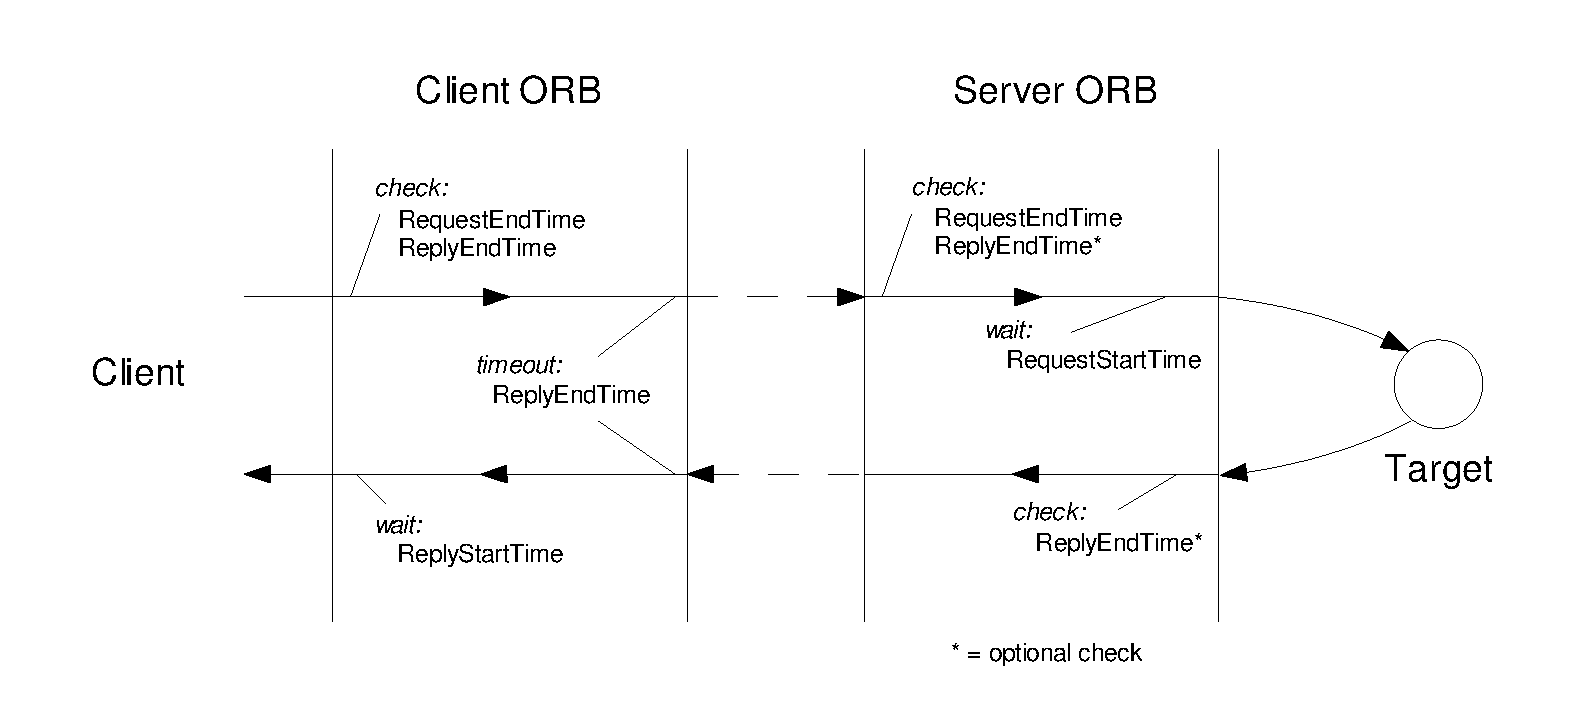
\includegraphics[width=16cm]{QoS/Timing}
  \end{center}
\caption{Timing Policies in JacORB}
\label{fig:timing}
\end{figure}

Figure \ref{fig:timing} shows how JacORB interprets the timing
policies in the course of a single request.

\begin{itemize}
\item As soon as the ORB receives control (prior to marshaling), it
converts any \emph{RelativeRequestTimeoutPolicy} or
\emph{RelativeRoundtripTimeoutPolicy} to an absolute value, by adding
the relative value to the current system time.

\item The ORB then checks whether \emph{Request End Time} or
\emph{Reply End Time} have already elapsed.  If so, no invocation is
made, and an {\tt org.omg.CORBA.TIMEOUT} is thrown to the client.

\item After the ORB has sent the request, it waits for a reply until
\emph{Reply End Time} has elapsed.  If it receives no reply before
that, the request is discarded and an {\tt org.omg.CORBA.TIMEOUT}
thrown to the client.  (JacORB does not currently cancel the
outstanding request, it simply discards the reply, should one arrive
after the timeout has elapsed.)\footnote{Note that if there is no
  connection to the server yet, other timeouts are applied first,
configured by the properties {\tt
  jacorb.connection.client.connect\_timeout} and {\tt
  jacorb.retries}.  If connection establishment fails, control does
not return to the client until these timeouts have expired, even if
this is later than \emph{Reply End Time}.}

\item On the server side (before demarshaling), the ORB checks whether
the \emph{Request End Time} has already elapsed.  If so, the request
is not delivered to the target, and an {\tt org.omg.CORBA.TIMEOUT}
is thrown back to the client.

\item Optionally, the server-side ORB may also check at this point
whether the \emph{Reply End Time} has already elapsed, and not
actually invoke the target in this case (throwing back an {\tt
org.omg.CORBA.TIMEOUT} to the client as well).  Since the \emph{Reply
  End Time} would then be checked both on the client and the server
side, this requires that the clocks on both machines are synchronized
at least to the same order of magnitude as the timeout itself.  This
check is therefore off by default, and may be enabled by setting the
property {\tt jacorb.poa.check\_reply\_end\_time} to ``on''.

\item If the request proceeds, the ORB waits until the \emph{Request
Start Time} has been reached, if one was specified, and has not
already elapsed.  After that, the request is delivered to the target.

\item After the target invocation has returned, the ORB may
optionally check whether the \emph{Reply End Time} has now elapsed.
Similar to the check prior to the target invocation, this check is
also optional and controlled by the property {\tt
jacorb.poa.check\_reply\_end\_time} (see discussion above).  If
the check is enabled, and the \emph{Reply End Time} is found to have
elapsed at this point, the ORB sends an {\tt org.omg.CORBA.TIMEOUT}
back to the client, rather than the actual reply.

\item If the reply arrives at the client before \emph{Reply End Time}
has elapsed, the ORB waits until \emph{Reply Start Time} has been
reached, if one was specified, and has not already elapsed.  After
that, the reply is delivered back to the client.

\end{itemize}

The bottom line of this is that for a simple, per-invocation timeout,
you should specify a \mbox{\emph{RelativeRoundtripTimeoutPolicy}}.

\clearpage{}
\subsection*{Programming}

In CORBA, points of time are specified to an accuracy of 100~nanoseconds, using
values of struct {\tt TimeBase::UtcT}.  To allow easy manipulation of such
values from Java, JacORB provides a number of static methods in {\tt
org.jacorb.util.Time}.  For example, to convert the current Java time
into a {\tt UtcT} value, write

\begin{verbatim}
UtcT currentTime = org.jacorb.util.Time.corbaTime();
\end{verbatim}

To create a {\tt UtcT} value that specifies a time $n$~milliseconds in the
future, you can write

\begin{verbatim}
UtcT time = org.jacorb.util.Time.corbaFuture (10000 * n);
\end{verbatim}

(The argument to {\tt corbaFuture()} is in CORBA time units of
100~ns; we multiply $n$ by 10000 here to convert it from Java time
units (milliseconds).)

The following shows how to set a timing policy for an object using the
standard mechanism (see the beginning of this chapter for an
explanation).  In this example, we set a \emph{Reply End Time} that
lies one second in the future:

\begin{verbatim}
import org.omg.CORBA.*;

SomeCorbaType server  = ...  // the object for which we want to set
                             // a timing policy
org.omg.CORBA.ORB orb = ...
org.omg.CORBA.Any a   = orb.create_any();

org.omg.TimeBase.UtcT replyEndTime
    = org.jacorb.util.Time.corbaFuture (1000 * 10000);  // one second

org.omg.TimeBase.UtcTHelper.insert (a, replyEndTime);

try
{
    Policy p
        = orb.create_policy (REPLY_END_TIME_POLICY_TYPE.value, a);
    server._set_policy_override (new Policy[]{ p },
                                 SetOverrideType.ADD_OVERRIDE);
}
catch (PolicyError e)
{
    ...
}
\end{verbatim}

\clearpage{}

Using the constructors of JacORB's implementations of policy values,
this becomes less verbose:

\begin{verbatim}
SomeCorbaType server  = ...

Policy p = new org.jacorb.orb.policies.ReplyEndTimePolicy
                   (org.jacorb.util.Time.corbaFuture (1000 * 10000));

server._set_policy_override (new Policy[]{ p },
                             SetOverrideType.ADD_OVERRIDE);
\end{verbatim}

Likewise, to set a \emph{Relative Roundtrip Timeout} of one second,
write:

\begin{verbatim}
SomeCorbaType server  = ...

Policy p =
    new org.jacorb.orb.policies.RelativeRoundtripTimeoutPolicy 
                                                      (1000 * 10000);

server._set_policy_override (new Policy[]{ p },
                             SetOverrideType.ADD_OVERRIDE);
\end{verbatim}

The difference between this and the example before, where a
\emph{Reply End Time} was used, is that the latter specifies a
\emph{relative time} to CORBA.  The policy will therefore be valid
for all subsequent invocations, because the absolute deadline will be
recomputed before each invocation.  In the first example, the
deadline will no longer make sense for any subsequent invocations,
since only an absolute time was specified to the ORB.


%%% Local Variables: 
%%% mode: latex
%%% TeX-master: "../ProgrammingGuide"
%%% End: 


%%%%%%%%%%%%%%%%%%%%%%%%%%%%%%%%%%%%%%%%%%%%%%%%%%%%%%%%%%%%%%%%%%%%%%%%%%%%%%

\chapter{Connection Management and Connection Timeouts}
\label{ch:connections}


JacORB offers a certain level of control over connections and timeouts. You
can
\begin{itemize}
\item set connection idle timeouts.
\item set request timing.
\item set the maximum number of accepted TCP/IP connections on the server.
\end{itemize}

\section{Timeouts}
\label{connection_timeouts}
Connection idle timeouts can be set individually for the client and the
server. They control how long an idle connection, i.e.~a connection that has
no pending replies, will stay open. The corresponding properties are {\tt
  jacorb.connection.client.idle\_timeout} and {\tt
  jacorb.connection.server.timeout} and take their values as milliseconds. If
not set, connections will stay open indefinitely (or until the OS decides to
close them).

\emph{Request timing} controls how long an individual request may take to
complete.  The programmer can specify this using QoS policies,
discussed in chapter \ref{ch:qos}.

\section{Connection Management}
\label{connection_management}

When a client wants to invoke a remote object, it needs to send the request
over a connection to the server. If the connection isn't present, it has to be
created. In JacORB, this will only happen once for every combination of host
name and port. Once the connection is established, all requests and replies
between client and server will use the same connection. This saves resources
while adding a thin layer of necessary synchronization, and is the recommended
approach of the OMG. Occasionally people have requested to allow for multiple
connections to the same server, but nobody has yet presented a good argument
that more connections would speed up things considerably.

On the server side, the property {\tt
  jacorb.connection.max\_server\_transports} allows to set the maximum number
of TCP/IP connections that will be listened on for requests. When using a
network sniffer or tools like netstat, more inbound TCP/IP connections than
the configured number may be displayed. This is for the following reason:
Whenever the connection limit is reached, JacORB tries to close existing idle
connections (see the subsection below). This is done on the thread
that accepts the new connections, so JacORB will not actively accept more
connections. However, the ServerSocket is initialized with a backlog of 20.
This means that 20 more connections will be quasi-accepted by the OS. Only the
21st will be rejected right away.

\subsection{Basics and Design}
\label{connection_management_basics}
Whenever there is the need to close an existing connection because of the
connection limit, the question arises on which of the connection to close. To
allow for maximum flexibility, JacORB provides the interface {\tt
  SelectionStrategy} that allows for a custom way to select a connection to
close. Because selecting a connection usually requires some sort of
statistical data about it, the interface {\tt
  StatisticsProvider} allows to implement a class that collects statistical
data.

\begin{small}
\begin{verbatim}
package org.jacorb.orb.giop;

public interface SelectionStrategy
{
    public ServerGIOPConnection
        selectForClose( java.util.List connections );
}

public interface StatisticsProvider
{
    public void messageChunkSent( int size );
    public void flushed();
    public void messageReceived( int size );
}
\end{verbatim}
\end{small}

The interface {\tt SelectionStrategy} has only the single method of {\tt
  selectForClose()}. This is called by the class {\tt GIOPConnectionManager}
when a connection needs to be closed. The argument is a {\tt List} containing
objects of type {\tt ServerGIOPConnection}. The call itself is synchronized in
the {\tt GIOPConnectionManager}, so no additional synchronization has to be
done by the implementor of {\tt SelectionStrategy}. When examining the
connections, the strategy can get hold of the {\tt StatisticsProvider} via the
method {\tt getStatisticsProvider()} of the class {\tt GIOPConnection}. The
strategy implementor should take care only to return idle connections. While
the connection state is checked anyway while closing (it may have changed in
the meantime), it seems to be more efficient to avoid cycling through the
connections. When no suitable connection is available, the strategy may
return {\tt null}. The {\tt GIOPConnectionManager} will then wait for a
configurable time, and try again. This goes on until a connection can be
closed.

The interface {\tt StatisticsProvider} is used to collect statistical data
about a connection and provide it to the {\tt SelectionStrategy}.  Because the
nature of this data may vary, there is no standard access to the data via the
interface. Therefore, {\tt StatisticsProvider} and {\tt SelectionStrategy}
usually need to be implemented together. Whenever a new connection is
created\footnote{Currently, connection management is only implemented for the
server side. Therefore, only accepted {\tt ServerGIOPConnections}s will get a
{\tt StatisticsProvider}}, a new {\tt StatisticsProvider} object is
instanciated and stored with the {\tt GIOPConnection}\footnote{This is
actually only done when a {\tt StatisticsProvider} is configured}.
The {\tt StatisticsProvider} interface is oriented along the mode of use of the {\tt
GIOPConnection}. For efficiency reasons, messages are not sent as one big byte
array. Instead, they are sent piecewise over the wire. When such a chunk is
sent, the method {\tt messageChunkSent(int size)} will be called. After the
message has been completely sent, method {\tt flush()} is called. This whole
process is synchronized, so all consecutive {\tt messageChunkSent}s until a
{\tt flush()} form a single message. Therefore, no synchronization on this
level is necessary. However, access to gathered statistical data by the {\tt
SelectionStrategy} is concurrent, so care has to be taken. Receiving messages
is done only on the whole, so there exists only one method, {\tt
messageReceived(int size)}, to notify the {\tt StatisticsProvider} of such an
event.


JacORB comes with two pre-implemented strategies: least frequently used and
least recently used. LFU and LRU are implemented by the classes {\tt
  org.jacorb.orb.giop.L[F|R]USelection\-StrategyImpl} and {\tt
  org.jacorb.orb.giop. L[F|R]U\-Statistics\-ProviderImpl}.

\subsection{Configuration}
\label{connection_management_config}
To configure connection management, the following properties are provided:
\begin{description}
\item {\tt jacorb.connection.max\_server\_connections} This property sets the
  maximum number of TCP/IP connections that will be listened on by the
  server--side ORB.
\item {\tt jacorb.connection.wait\_for\_idle\_interval} This property sets the
  interval to wait until the next try is made to find an idle connection to
  close. Value is in microseconds.
\item {\tt jacorb.connection.selection\_strategy\_class} This property sets
  the {\tt Selection\-Strategy}.
\item {\tt jacorb.connection.statistics\_provider\_class} This property sets
  the {\tt Statistics\-Provider}.
\item {\tt jacorb.connection.delay\_close} If turned on, JacORB will delay
  closing of TCP/IP connections to avoid certain situations, where message
  loss can occur. See also section \ref{connection_management_limitations}.
\end{description}

\subsection{Limitations}
\label{connection_management_limitations}
When trying to close a connection, it is first checked that the connection is
idle, i.e.~has no pending messages.  If this is the case, a GIOP
CloseConnection message is sent, and the TCP/IP connection is closed. Under
high load, this can lead to the following situation:

\begin{enumerate}
\item Server sends the CloseConnection message.
\item Server closes the TCP/IP connection.
\item The client sends a new request into the connection, because it hasn't
  yet read and acted on the CloseConnection message.
\item The server--side OS will send a TCP RST, which cancels out the
  CloseConnection message.
\item The client finds the connection closed and must consider the request lost.
\end{enumerate}

To get by this situation, JacORB takes the following approach. Instead
of closing the connection right after sending the CloseConnection
message, we delay closing and wait for the client to close the
connection. This behaviour is turned off by default, but can be
enabled by setting the property {\tt jacorb.connection.delay\_close}
to ``yes''. When non-JacORB clients are used care has to be taken that
these ORBs do actively close the connection upon receiving a
CloseConnection message.


%%% Local Variables:
%%% mode: latex
%%% TeX-master: "../ProgrammingGuide"
%%% End:


%%%%%%%%%%%%%%%%%%%%%%%%%%%%%%%%%%%%%%%%%%%%%%%%%%%%%%%%%%%%%%%%%%%%%%%%%%%%%%

\chapter{Extensible Transport Framework}
\label{ch:etf}


The \emph{Extensible Transport Framework (ETF)}, which JacORB
implements, allows you to plug in other transport layers besides the
 standard IIOP (TCP/IP) protocol\footnote{At the time of
 this writing (July 2003), ETF is still a draft standard (OMG TC
 document mars/2003-02-01).}.

To use an alternative transport, you need to (a) implement it as a set
of Java classes following the ETF specification, and (b) tell JacORB
to use the new transport instead of (or alongside with) the standard
IIOP transport.  We cover both steps below.

\section{Implementing a new Transport}

The interfaces that an ETF-compliant transport must implement are
 described in the ETF specification, and there is thus no need to
 repeat that information here.  JacORB's default IIOP transport, which
 is realized in the package {\tt org.jacorb.orb.iiop}, can also serve
 as a starting point for implementing your own transports.

For each transport, the following interfaces must be implemented
(defined in {\tt ETF.idl}, the package is {\tt org.omg.ETF}):

\begin{description}
\item[Profile] encapsulates addressing information for this transport
\item[Listener] server-side communication endpoint, waits for incoming
connections and passes them up to the ORB
\item[Connection] an actual communication channel for this transport
\item[Factories] contains factory methods for the above interfaces
\end{description}

The {\tt Handle} interface from the ETF package is implemented in the
 ORB (by the class {\tt org.jacorb.orb.BasicAdapter}), not by
 individual transports.  There is currently no support in JacORB for
 the optional zero-copy mechanism; the interface {\tt
 ConnectionZeroCopy} therefore needn't be implemented.

On the server side, the {\tt Listener} must pass incoming connections
 up to the ORB using the ``Handle'' mechanism; the {\tt accept()}
 method needn't be implemented.  Once a {\tt Connection} has been
 passed up to the ORB, it will never be ``returned'' to the {\tt
 Listener} again.  The method {\tt completed\_data()} in the {\tt
 Listener} interface therefore needn't be implemented, and neither
 should the {\tt Listener} ever call {\tt
 Handle.signal\_data\_available()} or {\tt Handle.closed\_by\_peer()}
 (these methods throw a {\tt NO\_IMPLEMENT} exception in JacORB).

At the time of this writing (July 2003), there is still uncertainty in
 ETF about how server-specific Profiles (as returned by {\tt
 Listener.endpoint()}, for example) should be turned into
 object-specific ones for inclusion into IORs.  We have currently
 added three new operations to the {\tt Profile} interface to resolve
 this issue, see JacORB's version of {\tt ETF.idl} for details.

\section{Configuring Transport Usage}

You tell JacORB which transports it should use by listing the names of
 their {\tt Factories} classes in the property {\tt
 jacorb.transport.factories}.  In the standard configuration, this
 property contains only {\tt org.jacorb.orb.iiop.IIOPFactories}, the
 {\tt Factories} class for the standard IIOP transport.  The
 property's value is a comma-separated list of fully qualified Java
 class names; each of these classes must be found somewhere on the
 CLASSPATH that JacORB is started with.  For example:

\begin{scriptsize}
\begin{verbatim}
jacorb.transport.factories = my.transport.Factories, org.jacorb.orb.iiop.IIOPFactories
\end{verbatim}
\end{scriptsize}

By default, a JacORB server creates listeners for each transport
listed in the above property, and publishes profiles for each of these
transports in any IOR it creates.  The order of profiles within an IOR
is the same as that of the transports in the property.

If you don't want your servers to listen on each of these transports
 (e.g. because you want some of your transports only to be used for
 client-side connections), you can specify the set of actual listeners
 in the property {\tt jacorb.transport.server.listeners}.  The value
 of this property is a comma-separated list of numeric profile tags,
 one for each transport that you want listeners for, and which you
 want published in IOR profiles.  The numeric value of a transport's
 profile tag is the value returned by the implementation of {\tt
 Factories.profile\_tag()} for that transport.  Standard IIOP has
 profile tag 0 ({\tt TAG\_INTERNET\_IOP}).  Naturally, you can only
 specify profile tag numbers here for which you have a corresponding
 entry in {\tt jacorb.transport.factories}.

So, to restrict your server-side transports to standard IIOP, you
would write:

\begin{verbatim}
jacorb.transport.server.listeners = 0
\end{verbatim}

On the client side, the ORB must decide which of potentially many
 transports it should use to contact a given server.  The default
 strategy is that for each IOR, the client selects \emph{the first profile
 for which there is a transport implementation available at the client
 side} (specified in {\tt jacorb.transport.factories}).  Profiles for
which the client has no transport implementation are skipped.

Note that this is a purely static decision, based on availability of
 an implementation.  JacORB does not attempt to actually establish a
 transport connection in order to find out which transport can be
 used.  Also, should the selected transport fail, JacORB does not
 ``fall back'' to the next transport in the list.  (This is because
 JacORB opens connections lazily, only when the first actual data is
 being sent.)

You can customize this strategy by providing your own implementation of
{\tt org.jacorb.orb.ProfileSelector}, and specifying it in the
property {\tt jacorb.transport.client.selector}.  The interface {\tt
ProfileSelector} requires a single method,

\begin{verbatim}
   public Profile selectProfile (List profiles,
                                 ClientConnectionManager ccm);
\end{verbatim}

For each IOR, this method receives a list of all profiles from the IOR
 for which the client has a transport implementation, in the order in
 which they appear in the IOR.  The method should select one profile
 from this list and return it; this profile will then be used for
 communication with the server.

To help with the decision, JacORB's {\tt ClientConnectionManager} is
 passed as an additional parameter.  The method implementation can use
 it to check whether connections with a given transport, or to a given
 server, have already been made; it can also try and pre-establish a
 connection using a given transport and store it in the {\tt
 ClientConnectionManager} for later use.  (See the JacORB source code
to find out how to deal with the {\tt ClientConnectionManager}.)

The default {\tt ProfileSelector} does not use the {\tt
 ClientConnectionManager}, it simply returns the first profile from
 the list, unconditionally.  To let JacORB use your own implementation
 of the {\tt ProfileSelector} interface, specify the fully qualified
 classname in the property:

\begin{verbatim}
jacorb.transport.client.selector=my.pkg.MyProfileSelector
\end{verbatim}


%%% Local Variables: 
%%% mode: latex
%%% TeX-master: "../ProgrammingGuide"
%%% End: 


%%%%%%%%%%%%%%%%%%%%%%%%%%%%%%%%%%%%%%%%%%%%%%%%%%%%%%%%%%%%%%%%%%%%%%%%%%%%%%

\chapter{Security Attribute Service}
\label{ch:sas}


The Security Attribute Service (SAS) is part of the Common Secure 
Interoperability Specification, Version 2 (CSIv2) CORBA specification.
It is defined in the Secure Interoperability chapter (chapter 24) of the
CORBA 3.0.2 Specification.

\section{Overview}

The SAS specification defines the interchange between a Client Security 
Service (CSS) and a Target Security Service (TSS)
for the exchange of security authentication and authorization
elements. This information is exchanged in the Service Context of the GIOP
request and reply messages. The SAS may be used in conjunction with SSL to
provide privacy of the messages being sent and received.

The SAS service is implemented as a series of standard CORBA interceptors,
one for the CSS and one for the TSS. The service also uses a user specified
SAS context class to support different authentication mechanisms, such as
GSSUP and Kerberos.

The SAS service is activated based on entries in the JacORB properties file.
The properties are slightly different for a CSS and a TSS application.

The following is a part of the JacORB properties file that is used by 
the CSS.

\begin{scriptsize}
\begin{verbatim}
########################################
#                                      #
#   SAS configuration                  #
#                                      #
########################################

# This option initializes SAS support in the ORB and sets the logging level
jacorb.security.support_sas=on
jacorb.SAS.log.verbosity=3

# This option configures the SAS to support stateful sessions (default=true)
jacorb.security.sas.tss.stateful=true

# This option defines the specific SAS context generator/validator
# Currently supported contexts include:
#    GssUpContext      - Uses GSSUP security
#    KerberosContext   - uses Kerberos security
jacorb.security.sas.contextClass=org.jacorb.security.sas.GssUpContext
#jacorb.security.sas.contextClass=org.jacorb.security.sas.KerberosContext

# This initializer installs the SAS Target Security Service (TSS)
#org.omg.PortableInterceptor.ORBInitializerClass.SASTarget=org.jacorb.security.sas.SASTargetInitializer

# This initializer installs the SAS Client Security Service (CSS)
org.omg.PortableInterceptor.ORBInitializerClass.SASClient=org.jacorb.security.sas.SASClientInitializer

# This option is used for GSSUP security and sets up the GSS Provider
org.omg.PortableInterceptor.ORBInitializerClass.GSSUPProvider=org.jacorb.security.sas.
GSSUPProviderInitializer

# This option identifies the layered security attributes required by the target
# Attributes are entered in a comma-separated list. Valid attributes are:
#       Integrity
#       Confidentiality
#       EstablishTrustInTarget
#       EstablishTrustInClient
#       IdentityAssertion
#       DelegationByClient
#jacorb.security.sas.tss.target_supports=EstablishTrustInTarget
#jacorb.security.sas.tss.target_requires=EstablishTrustInTarget
\end{verbatim}
\end{scriptsize}


The following is a part of the JacORB properties file that is used by 
the TSS.

\begin{scriptsize}
\begin{verbatim}
########################################
#                                      #
#   SAS configuration                  #
#                                      #
########################################

# This option initializes SAS support in the ORB and sets the logging level
jacorb.security.support_sas=on
jacorb.SAS.log.verbosity=3

# This option configures the SAS to support stateful sessions (default=true)
jacorb.security.sas.tss.stateful=true

# This option defines the specific SAS context generator/validator
# Currently supported contexts include:
#    GssUpContext      - Uses GSSUP security
#    KerberosContext   - uses Kerberos security
jacorb.security.sas.contextClass=org.jacorb.security.sas.GssUpContext
#jacorb.security.sas.contextClass=org.jacorb.security.sas.KerberosContext

# This initializer installs the SAS Target Security Service (TSS)
org.omg.PortableInterceptor.ORBInitializerClass.SASTarget=org.jacorb.security.sas.SASTargetInitializer

# This initializer installs the SAS Client Security Service (CSS)
#org.omg.PortableInterceptor.ORBInitializerClass.SASClient=org.jacorb.security.sas.SASClientInitializer

# This option is used for GSSUP security and sets up the GSS Provider
org.omg.PortableInterceptor.ORBInitializerClass.GSSUPProvider=org.jacorb.security.sas.
GSSUPProviderInitializer

# This option identifies the layered security attributes required by the target
# Attributes are entered in a comma-separated list. Valid attributes are:
#       Integrity
#       Confidentiality
#       EstablishTrustInTarget
#       EstablishTrustInClient
#       IdentityAssertion
#       DelegationByClient
jacorb.security.sas.tss.target_supports=EstablishTrustInTarget
jacorb.security.sas.tss.target_requires=EstablishTrustInTarget
\end{verbatim}
\end{scriptsize}

In some cases, an application may act as both a CSS and a TSS. 
In these cases, a single properties file may be used with both the
CSS and TSS interceptors included.

\section{GSSUP Example}

The GSSUP (GSS Username/Password) example demonstraites the simplest 
usage of the SAS service. In this example, username and password
pairs are send via the SAS service. The client registers its username
and password with the GSSUP Context which is later used CSS interceptor
to generate the user's authentication information.
The TSS retrieves the username and password
without validating them. It is assumed by the TSS that the username
and password are correct and/or will be further validated by a later
interceptor or application code.

The following describes a SAS example using GSSUP.

\subsection{GSSUP IDL Example}

\begin{scriptsize}
\begin{verbatim}
module demo{
  module sas{
    interface SASDemo{
      void printSAS();
    };
  };
};
\end{verbatim}
\end{scriptsize}

The IDL contains a single interface. This interface is used to print out
the user principal sent and received by the SAS service.

\subsection{GSSUP Client Example}

The following is a sample GSSUP client.

\begin{scriptsize}
\begin{verbatim}
package demo.sas;

import java.io.BufferedReader;
import java.io.File;
import java.io.FileReader;

import org.jacorb.security.sas.GssUpContext;
import org.omg.CORBA.ORB;

public class GssUpClient {
    public static void main(String args[]) {
        if (args.length != 3) {
            System.out.println("Usage: java demo.sas.GssUpClient <ior_file> <username> <password>");
            System.exit(1);
        }

        try {
            // set security credentials
            GssUpContext.setUsernamePassword(args[1], args[2]);

            // initialize the ORB.
            ORB orb = ORB.init(args, null);

            // get the server
            File f = new File(args[0]);
            if (!f.exists()) {
                System.out.println("File " + args[0] + " does not exist.");
                System.exit(-1);
            }
            if (f.isDirectory()) {
                System.out.println("File " + args[0] + " is a directory.");
                System.exit(-1);
            }
            BufferedReader br = new BufferedReader(new FileReader(f));
            org.omg.CORBA.Object obj = orb.string_to_object(br.readLine());
            br.close();
            SASDemo demo = SASDemoHelper.narrow(obj);

            //call single operation
            demo.printSAS();
            demo.printSAS();
            demo.printSAS();

            System.out.println("Call to server succeeded");
        } catch (Exception ex) {
            ex.printStackTrace();
        }
    }
}
\end{verbatim}
\end{scriptsize}

The key to the client is the call to:
\begin{scriptsize}
\begin{verbatim}
    GssUpContext.setUsernamePassword(args[1], args[2]);
\end{verbatim}
\end{scriptsize}
This call registers the client's username and password with the GSSUP context.
This information will then later be used by the CSS interceptor as the user's
authentication information.

The following is JacORB properties section for the client SAS.

\begin{scriptsize}
\begin{verbatim}
jacorb.security.support_sas=on
jacorb.SAS.log.verbosity=3
jacorb.security.sas.tss.stateful=true
jacorb.security.sas.contextClass=org.jacorb.security.sas.GssUpContext
org.omg.PortableInterceptor.ORBInitializerClass.SASClient=org.jacorb.security.sas.SASClientInitializer
org.omg.PortableInterceptor.ORBInitializerClass.GSSUPProvider=org.jacorb.security.sas.GSSUPProviderInitializer
\end{verbatim}
\end{scriptsize}

\subsection{GSSUP Target Example}

The following is a sample GSSUP target.

\begin{scriptsize}
\begin{verbatim}
package demo.sas;

import java.io.FileWriter;
import java.io.PrintWriter;

import org.jacorb.security.sas.GssUpContext;
import org.omg.PortableServer.POA;
import org.omg.CORBA.ORB;

public class GssUpServer extends SASDemoPOA {
    private ORB orb;

    public GssUpServer(ORB orb) {
        this.orb = orb;
    }

    public void printSAS() {
        try {
            org.omg.PortableInterceptor.Current current = 
                (org.omg.PortableInterceptor.Current) orb.resolve_initial_references("PICurrent");
            org.omg.CORBA.Any anyName = 
                current.get_slot(org.jacorb.security.sas.SASTargetInitializer.sasPrincipalNamePIC);
            String name = anyName.extract_string();
            System.out.println("printSAS for user " + name);
        } catch (Exception e) {
            System.out.println("printSAS Error: " + e);
        }
    }

    public static void main(String[] args) {
        if (args.length != 1) {
            System.out.println("Usage: java demo.sas.GssUpServer <ior_file>");
            System.exit(-1);
        }

        try {
            // initialize the ORB and POA.
            ORB orb = ORB.init(args, null);
            POA poa = (POA) orb.resolve_initial_references("RootPOA");
            poa.the_POAManager().activate();
			
            // create object and write out IOR
            org.omg.CORBA.Object demo = poa.servant_to_reference(new GssUpServer(orb));
            PrintWriter pw = new PrintWriter(new FileWriter(args[0]));
            pw.println(orb.object_to_string(demo));
            pw.flush();
            pw.close();
			
            // run the ORB
            orb.run();
        } catch (Exception e) {
            e.printStackTrace();
        }
    }
}
\end{verbatim}
\end{scriptsize}

The following is JacORB properties section for the target SAS.

\begin{scriptsize}
\begin{verbatim}
jacorb.security.support_sas=on
jacorb.SAS.log.verbosity=3
jacorb.security.sas.tss.stateful=true
jacorb.security.sas.contextClass=org.jacorb.security.sas.GssUpContext
org.omg.PortableInterceptor.ORBInitializerClass.SASTarget=org.jacorb.security.sas.SASTargetInitializer
org.omg.PortableInterceptor.ORBInitializerClass.GSSUPProvider=org.jacorb.security.sas.GSSUPProviderInitializer
jacorb.security.sas.tss.target_supports=EstablishTrustInTarget
jacorb.security.sas.tss.target_requires=EstablishTrustInTarget
\end{verbatim}
\end{scriptsize}

%%% Local Variables: 
%%% mode: latex
%%% TeX-master: "../ProgrammingGuide"
%%% End: 


%%%%%%%%%%%%%%%%%%%%%%%%%%%%%%%%%%%%%%%%%%%%%%%%%%%%%%%%%%%%%%%%%%%%%%%%%%%%%%

\chapter{The JacORB Notification Service}
\label{ch:ntfy}

%
% $Id$
%

The JacORB Notification Service is a partial implementation of
the Notification Service specified by the OMG.

\section{Running the Notification Service}
\label{sec:ntfy-running}

Before the JacORB Notification Service can be accessed a server
process must be started. Starting
the notification server is done by running

\cmdline{ntfy [-printIOR] [-printCorbaloc] [-writeIOR <filename>]
  [-registerName <nameID>[.<nameKind>]] [-port <oaPort>] [-channels
  <channels>] [-help]} 


\subsection{Running as a NT Service or a UNIX Daemon}
\label{sec:runn-notif-serv-1}

With a little help from
\href{http://wrapper.tanukisoftware.org}{the Java Service Wrapper} it is
easy to run the JacORB notification service as a Windows Service or as
a UNIX daemon. 

\subsubsection{Installing and Running as a NT Service}
\label{sec:windows-service}

The necessary wrapper configuration files are preconfigured in the
\texttt{JacORB/bin} directory. 

The notification service can be installed as a service by double
clicking on the \texttt{NotifyService-Install-NT.bat} batch file which
is located in the \texttt{JacORB/bin} directory.
Alternatively you can open a Command Window and then run the install
script from the command prompt. 

\begin{verbatim}
  C:\JacORB\bin>NotifyService-Install-NT.bat
  wrapper  | JacORB Notification Service installed.
\end{verbatim}

Once the service has been installed, it can be started by opening up
the Service Control Panel, selecting the service, and then pressing
the start button.

The service can also be started and stopped from within a Command
Window by using the \texttt{net start JacORB-Notify} and \texttt{net
  stop JacORB-Notify} commands, or 
by passing commands to the Wrapper.exe executable. 

The wrapper is set up to start the JacORB Notification Service
whenever the machine is rebooted.

The service can be uninstalled by running the
\texttt{NotifyService-Uninstall-NT.bat} batch file.

See the Windows specific
\href{http://wrapper.tanukisoftware.org/doc/english/launch-win.html}{wrapper
  documentation} for more details.
  

\subsubsection{Installing and Running as a UNIX Daemon}
\label{sec:inst-runn-as}

JacORB is shipped with a \texttt{sh} script which can be used to start
and stop the JacORB Notification Service controlled by the Java
Service Wrapper.

First you need to download the appropiate binary for your system from
\href{http://wrapper.tanukisoftware.org}{http://wrapper.tanukisoftware.org}.
The Java Service Wrapper is supported on Windows, Linux, Solaris, AIX,
HP-UX, Macintosh OS X, DEC OSF1, FreeBSD, and SGI Irix systems (Note:
You don't need to download anything if you are running Windows. All
necessary stuff is shipped with the JacORB distribution).

You'll need two files from the downloaded distribution. One is
the system-specific \texttt{wrapper} executable. Place it somewhere in
your searchpath. The second is the native library
\texttt{libwrapper.so} in the \texttt{\emph{wrapper-dir}/lib}
directory. This library is required by the 
wrapper executable. Place the library in the \texttt{JacORB/lib}
directory. Alternatively you can create a link to the library.

Ensure that the shell-script
\texttt{JacORB/bin/ntfy-wrapper} has the executable bit set. Note that
the sh script will attempt to create a pid file in the directory
specified by the property \texttt{PIDDIR} in the script. If
the user used to launch the Wrapper does not have permission to write
to this directory then this will result in an error. An alternative
that will work in most cases is to write the pid file to another
directory. To make this change, edit the sh  script and change the following line: 

\begin{verbatim}
PIDDIR="."
\end{verbatim}
to something more appropiate:
\begin{verbatim}
PIDDIR="/var/run"
\end{verbatim}


\paragraph{Running in the console}
\label{sec:running-console}

 The JacORB notification service  can now be run by simply executing
 \texttt{bin/ntfy-wrapper console}.

 When running using the console command, output from the notification
 service will be visible in the console. 

 The notification service can be terminated by hitting CTRL-C in the command
 window. This will cause the Wrapper to shut down the service cleanly.  

 If you omit the command the scripts prints the available commands.
 The script accepts the commands start, stop, restart and dump. The
 start, stop, and restart commands are common to most daemon scripts
 and are used to control the wrapper and the notification service  as
 a daemon process. The console 
 command will launch the wrapper in the current shell, making it
 possible to kill the application with CTRL-C. The final command,
 dump, will send a kill -3 signal to the wrapper causing the its JVM
 to do a full thread dump.  
 
 \paragraph{Running as a Daemon Process}
 \label{sec:running-as-daemon}
 
 The application can be run as a detatched daemon process by executing
 the script using the \emph{start} command. 

 When running using the start  command, output from the JVM will only
 be visible by viewing the logfile \texttt{NotifyService-Wrapper.log}
 using \texttt{tail -f NotifyService-Wrapper.log}. The location of the
 logfile can be configured in the wrapper configuration file
 \texttt{bin/NotifyService-Wrapper.conf} 

 Because the application is running as a detatched process, it can not
 be terminated using CTRL-C and will continue to run even if the
 console is closed. 
 
 To stop the application rerun the script using the \emph{stop} command.

 
 \paragraph{Installing The Application To Start on Reboot}
 \label{sec:inst-appl-start}

 This is system specific. See the UNIX specific
 \href{http://wrapper.tanukisoftware.org/doc/english/launch-nix.html}{wrapper
   documentation} for instructions for some platforms.

\section{Accessing the Notification Service}
\label{sec:access-notif-serv}

Configuring a default notification service as the ORB's default is done
by adding the URL that points to the service to the properties files
\texttt{.jacorb\_properties}. A valid URL can be obtained in various ways:

\begin{enumerate}
\item By specifying the option \texttt{-printIOR} as you start the
  notification service a stringified IOR is printed out to the
  console. From there you can copy it to a useful location.

\item Usually the stringified IOR makes most sense inside a file. Use
  the option \texttt{-writeIOR <filename>} to write the IOR to the specified
  file.

\item A more compact URL can be obtained by using the
  option \texttt{-printCorbaloc}. In conjunction with the option
  \texttt{-port} you can use the simplified corbaloc: URL of the form
  \texttt{corbaloc::ip-address:port/NotificationService}. This means
  all you need to know to construct an object reference to your
  notification service is the IP address of the machine and the port
  number the server process ist listening on (the one specified using
  \texttt{-port}). 

\end{enumerate}

Add the property \texttt{ORBInitRef.NotificationService} to your
properties file. The value can be a corbaloc: URL or alternatively the
file name where you saved the IOR.

The JacORB notification service is accessed using the standard CORBA
defined interface:

\small{
\begin{verbatim}
  // get a reference to the notification service
  ORB orb = ORB.init(args, null);
  org.omg.CORBA.Object obj; 
  obj = orb.resolve_initial_references("NotificationService");
  EventChannelFactory ecf = EventChannelHelper.narrow( o );
  IntHolder ih = new IntHolder();
  Property[] p1 = new Property[0];
  Property[] p2 = new Property[0];
  EventChannel ec = ecf.create_channel(p1, p2, ih);
  ...
\end{verbatim}
}

\section{Configuration}
\label{sec:ntfy-configuration}

Following is a brief description of the properties
that control Notification Service behaviour.

The Notification Service uses up to three Thread Pools with a configurable
size. The first Thread Pool is used to process the filtering of the
Messages. The second Thread Pool is used to deliver the Messages to the
Consumers. The third Thread Pool us used to pull Messages from PullSuppliers. 

\begin{small}
  \begin{longtable}{|p{5cm}|p{7.5cm}|p{1.5cm}|p{1.5cm}|}
    \caption{Notification Service Properties}\\
    \hline
    ~ \hfill \textbf {Property} \hfill ~ & ~ \hfill \textbf {Description}
    \hfill ~ & ~ \hfill \textbf {Type} \hfill ~ & \hfill \textbf{Default} \endhead
    \hline
    \verb"filter."
    \verb"thread_pool_size"\footnote{All notification service
    properties share the common prefix \emph{jacorb.notification} which
    is omitted here to save some space} &

    This is the Size of the Thread Pool used to process the filters.
    Increasing this value on a Multiprocessor machine or if Filters are on
    a different machine than the Channel could increase the Filtering
    Performance as multiple events can be processed concurrently. & 
    
    int $\geq$ 0 &

    2 \\
    \hline

    \verb"proxysupplier."
    \verb"thread_pool_size" &

    This is the Size of the Thread Pool used to deliver the Messages to
    the Consumers. By using the property
    \texttt{proxysupplier.threadpolicy}\footnote{also abbreviated.}
    it is also possible to use one Thread per ProxySupplier. &

    int $\geq$ 0 & 
    4 \\ \hline    

    \verb"proxyconsumer."
    \verb"thread_pool_size" &

    Specifies the Size of the Thread Pool used to pull Messages from
    PullSuppliers &

    int $>=$ 0 & 

    2 \\ \hline

    \verb"proxysupplier."
    \verb"threadpolicy" &

    Specify which thread policy the ProxySuppliers should use to deliver
    the Messages to its Consumers. Valid values are: 
    \begin{description}     
    \item[ThreadPool] a fixed number of threads is used. See property
      \verb"proxysupplier."
      \verb"thread_pool_size".

    \item[ThreadPerProxy] Each ProxySupplier uses its own thread.
      
    \end{description} & 
    string & Thread\-Pool \\ \hline

    \verb"supplier."
    \verb"poll_intervall" &

    Specifies how often Messages should be pulled from a PullSupplier. The
    value specifies the intervall between two pull-Operations. &

    milli\-seconds & 1000 \\ \hline

    \verb"supplier."
    \verb"max_number" &

    Specify the maximum number of Suppliers that may be connected to a
    Channel at a time. If a Supplier tries to connect, while this
    limit is exceeded, AdminLimitExceeded is raised. Note that this
    property can also be set programatically via the \texttt{set\_admin}
    operation. & int $>$ 0 & maximum int value \\ \hline

    \verb"consumer"
    \verb"max_number" &

    Specify the maximum number of Consumers that may be connected to a
    Channel at a time. If a Consumer tries to connect, while this
    limit is exceeded, AdminLimitExceeded is raised. Note that this
    property can also be set programatically via the
    \texttt{set\_admin} operation. &

    int $>$ 0 & maximum int value \\ \hline

    \verb"max_events_"
    \verb"per_consumer" &

    Specifies how many Events a ProxySupplier at most should queue for a
    consumer. If this number is exceeded Events are discarded according to
    the DiscardPolicy configured for the ProxySupplier. &

    int $>$ 0 & 100 \\ \hline

    \verb"max_batch_size" &

    Specifies the maximal number of Messages a SequencePushSupplier should
    queue before a delivery to its connected SequencedPushConsumer is
    forced. &

    int $>=0$ & 1 \\ \hline

    \verb"order_policy" &

    Specify how events that are queued should be ordered. Valid values
    are: 
    \begin{itemize}
    \item AnyOrder

    \item PriorityOrder

    \item DeadlineOrder

    \item FifoOrder
    \end{itemize} & 

    string & Priority\-Order \\ \hline

    \verb"discard_policy" &

    Specifies which Events are discarded if more than the  
    maximal number of events are queued for a consumer. 
    Valid values are:
    \begin{itemize}
    \item AnyOrder

    \item PriorityOrder

    \item DeadlineOrder

    \item FifoOrder

    \item LifoOrder
    \end{itemize} &

    string & Priority\-Order \\ \hline
       
    \verb"consumer."
    \verb"backout_interval" &

    After a delivery to a Consumer has failed the Channel will pause
    delivery to that Consumer for a while before retrying. This property
    specifies how long a consumer should stay disabled. &

    milli\-seconds & 1000 \\ \hline

    \verb"consumer."
    \verb"error_threshold" &

    Each failed delivery to a consumer increments an errorcounter. If this
    errorcounter exceeds the specified value the consumer is
    disconnected from the channel. &

    int $>=$ 0 & 3 \\ \hline

    \verb"default_filter_factory" &

    Specify which FilterFactory (\texttt{CosNotifyFilter::FilterFactory}) the
    attribute \texttt{EventChannel::\-default\_filter\_factory} should be set to. 
    Default value is \emph{builtin}. This special value implies that a
    FilterFactory will be created during start of the EventChannel.
    Its possible to set this property to a URL that points to another
    \texttt{CosNotifyFilter::FilterFactory} object. In this case no FilterFactory
    is started by the EventChannel. The URL is resolved by a call
    to \texttt{ORB::string\_to\_object}. &

    URL & builtin \\ \hline

    \verb"proxy.destroy_"
    \verb"causes_disconnect" &

    Specify if a destroyed Proxy should call the disconnect operation
    of its consumer/supplier. &

    boolean & on \\ \hline

 

  \end{longtable}
\end{small}


%%% Local Variables: 
%%% mode: latex
%%% TeX-master: "../ProgrammingGuide"
%%% End: 


%%%%%%%%%%%%%%%%%%%%%%%%%%%%%%%%%%%%%%%%%%%%%%%%%%%%%%%%%%%%%%%%%%%%%%%%%%%%%%

\chapter{Using Java management Extentions (JMX)}
\label{ch:jmx}


This section describes how to use the Java Management Extention API along with JacORB to
instrument both the orb and application that use JacORB.

\section{MX4J and JMX over IIOP}

This section describes how to instrument a JacORB application using the MX4J JMX implementation.
MX4J is an open source JMX implementation available at http://mx4j.sourceforge.net. This section
also shows how to use JMX over IIOP. This allows JMX to use an existing JacORB ORB for RMI
communications and the JacORB Naming Service to register you JMX MBeanServer.

To setup the JVM environment, three system defines are neccessary:

\begin{scriptsize}
\begin{verbatim}
-Djava.naming.factory.initial=com.sun.jndi.cosnaming.CNCtxFactory
-Djava.naming.provider.url=corbaloc:iiop:localhost:9101/StandardNS/NameServer-POA/_root
-Djavax.rmi.CORBA.PortableRemoteObjectClass=org.jacorb.orb.rmi.PortableRemoteObjectDelegateImpl
\end{verbatim}
\end{scriptsize}

The first system property tells the Java JNDI subsystem to use the CORBA Naming Service for its
naming repository. The second property is a pointer to the JacORB Naming Service instance. The
third property tells the Java Remote object system to use JacORB's Portable Remote Object implementation. This is required so that JacORB can associate an RMI object with a CORBA object on one of its POAs.

The sample code for creating a MBeanServer is shown below

\begin{scriptsize}
\begin{verbatim}
// The MBeanServer to which the JMXConnectorServer will be registered in
jmxServer = MBeanServerFactory.createMBeanServer();

// The address of the connector
HashMap environment = new HashMap();
org.jacorb.orb.rmi.PortableRemoteObjectDelegateImpl.setORB(orb);
JMXServiceURL address = new JMXServiceURL("service:jmx:iiop://localhost/jndi/jmxSnmpTrapNotify");
JMXConnectorServer cntorServer = JMXConnectorServerFactory.newJMXConnectorServer(address,                                             environment, jmxServer);

// Add MBeans
jmxServer.registerMBean(trapReceiver, new ObjectName("TrapReceiver:counts=default"));

// Start the JMXConnectorServer
cntorServer.start();
\end{verbatim}
\end{scriptsize}

The first line creates the MBeanServer.
The next 4 lines creates the remote JMX connection. The "`setORB()"' call assignes a previously
initialized ORB to the Remote Object delegate. All RMI over IIOP communications will occure
via this ORB. The "`address"' is the name of the MBeanServer as known in the Naming service.
The portion after "`/jndi/"' is the Naming Service name.
The next line registers a MBean with the MBeanServer.
The last line starts the MBeanServer.

A JMX console may then be used to monitor the JacORB application. For example, MC4J (http://mc4j.sourceforge.net) may be used. When setting up a mc4j connection, use the connection type JSR160 and set the server URL to the name as registered in the JacORB naming service, such as
"`service:jmx:iiop://localhost/jndi/jmxSnmpTrapNotify"'.

%%% Local Variables:
%%% mode: latex
%%% TeX-master: "../ProgrammingGuide"
%%% End:



%%%%%%%%%%%%%%%%%%%%%%%%%%%%%%%%%%%%%%%%%%%%%%%%%%%%%%%%%%%%%%%%%%%%%%%%%%%%%%

%%%%%%%%%%%%%%%%%%%%%%%%%%%%%%%%%%%%%%%%%%%%%%%%%%%%%%%%%%%%%%%%%%%%%%%%%%%%%%

\chapter{Transport Current}
\label{ch:transportcurrent}

%
% $Id$ 
%

Using the org.jacorb.transport.Current Feature

\emph{by Iliyan Jeliazkov}

\section{Scope and Context}

There is no standard-mandated mechanism to facilitate obtaining statistical or pretty 
much any operational information about the network transport which the ORB is using. 
While this is a direct corollary of the CORBA's design paradigm which mandates hiding 
all this hairy stuff behind non-transparent abstractions, it also precludes effective 
ORB and network monitoring. 

The Transport::Current feature intends to fill this gap by defining a framework 
for developing a wide range of solutions to this problem. It also provides a basic 
implementation for the most common case - the IIOP transport. 

By definition, transport-specific information is available in contexts where the 
ORB has selected a Transport:

\begin{itemize}
\item Within Client-side interception points; 
\item Within Server-side interception points; 
\item Inside a Servant up-call 
\end{itemize}

The implementation is based on a generic service-oriented framework, implementing 
the Transport::Current interface. It is an optional service, which can be dynamically l
oaded. This service makes the Transport::Current interface available through 
orb->resolve\_initial\_references() . The basic idea is simple - whenever a Transport 
is chosen by the ORB, the Transport::Current (or a protocolo-specific derivative) 
will have access to that instance and be able to provide some useful information. 



\section{Programmer's Reference}

Consider the following IDL interface to access transport-specific data. 

\begin{verbatim}
module org
{

  module jacorb
  {

    module transport
    {
      /// A type used to represent counters
      typedef unsigned long long CounterT;

      // Used to signal that a call was made outside the
      // correct invocation context.

      exception NoContext
      {
      };

      // The main interface, providing access to the Transport-specific
      // information (traits), available to the current thread of
      // execution.

      local interface Current
      {
          /// Transport ID, unique within the process.
        long id() raises (NoContext);

          /// Bytes sent/received through the transport.
          CounterT bytes_sent() raises (NoContext);
          CounterT bytes_received() raises (NoContext);

          /// Messages (requests and replies) sent/received using the current
          /// protocol.
          CounterT messages_sent() raises (NoContext);
          CounterT messages_received() raises (NoContext);

          /// The absolute time (miliseconds) since the transport has been
          /// open.
          TimeBase::TimeT open_since() raises (NoContext);
      };

    };

  };

};
\end{verbatim}

As an example of a specialized Transport::Current is the Transport::IIOP::Current, 
which derives from Transport::Current and has an interface, described in the following IDL: 

\begin{verbatim}
module org
{

  module jacorb
  {

    module transport
    {
      /// A type used to represent counters
      typedef unsigned long long CounterT;

      // Used to signal that a call was made outside the
      // correct invocation context.

      exception NoContext
      {
      };

      // The main interface, providing access to the Transport-specific
      // information (traits), available to the current thread of
      // execution.

      local interface Current
      {
          /// Transport ID, unique within the process.
        long id() raises (NoContext);

          /// Bytes sent/received through the transport.
          CounterT bytes_sent() raises (NoContext);
          CounterT bytes_received() raises (NoContext);

          /// Messages (requests and replies) sent/received using the current
          /// protocol.
          CounterT messages_sent() raises (NoContext);
          CounterT messages_received() raises (NoContext);

          /// The absolute time (miliseconds) since the transport has been
          /// open.
          TimeBase::TimeT open_since() raises (NoContext);
      };

    };

  };

};
\end{verbatim}


\section{User's Guide}

The org.jacorb.transport.Current can be used as a base interface for a more 
specialized interfaces. Iowever, it is not required that a more specialized 
Current inherits from it. 

Typical, generic usage is shown in the 
tests/regression/src/org/jacorb/test/transport/IIOPTester.java test: 

\begin{verbatim}
...
   // Get the Current object.
   Object tcobject = 
      orb.resolve_initial_references ("JacOrbIIOPTransportCurrent");
   Current tc = CurrentHelper.narrow (tcobject);

   logger.info("TC: ["+tc.id()+"] from="+tc.local_host() +":"
                + tc.local_port() +", to=" 
                +tc.remote_host()+":"+tc.remote_port());

   logger.info("TC: ["+tc.id()+"] sent="+tc.messages_sent ()
                + "("+tc.bytes_sent ()+")"
                + ", received="+tc.messages_received ()
                + "("+tc.bytes_received ()+")");
...
\end{verbatim}

\subsection{Configuration, Bootstrap, Initialization and Operation}


To use the Transport Current features the framework must be loaded 
through the Service Configuration framework. For example, using something 
like this: 

\begin{verbatim}
...
        Properties serverProps = new Properties();

        // We need the TC functionality
        serverProps.put ("org.omg.PortableInterceptor.ORBInitializerClass.
                             server_transport_current_interceptor",
                         "org.jacorb.transport.TransportCurrentInitializer");

        serverProps.put ("org.omg.PortableInterceptor.ORBInitializerClass.
                             server_transport_current_iiop_interceptor",
                        "org.jacorb.transport.IIOPTransportCurrentInitializer");

        serverORB = ORB.init(new String[0], serverProps);
...
\end{verbatim}

The ORB initializer registers the "JacORbIIOPTransportCurrent" name with the orb, 
so that it could be resolved via orb->resolve\_initial\_references("JacORbIIOPTransportCurrent"). 

Note that any number of transport-specific Current interfaces may be available at any one time. 



%%%%%%%%%%%%%%%%%%%%%%%%%%%%%%%%%%%%%%%%%%%%%%%%%%%%%%%%%%%%%%%%%%%%%%%%%%%%%%

%%%%%%%%%%%%%%%%%%%%%%%%%%%%%%%%%%%%%%%%%%%%%%%%%%%%%%%%%%%%%%%%%%%%%%%%%%%%%%

\chapter{JacORB Utilities}
\label{ch:tools}

%
% $Id$
%

In this chapter we  briefly explain the executables that come
with JacORB. These include the IDL-compiler, a utility to decode IORs
and print their components, the JacORB name server, a utility to test
a remote object's liveness, etc.

\section{idl}

The IDL compiler parses IDL files and maps type definitions to Java
classes as specified by the OMG IDL/Java language mapping. For
example, IDL interfaces are translated into Java interfaces, and
typedefs, structs, const declarations etc.  are mapped onto
corresponding Java classes. Additionally, stubs and skeletons for all
interface types in the IDL specification are generated.

(The  IDL  parser  was   generated  with  Scott  Hudson's  CUP  parser
generator.  The  LALR grammar for  the CORBA IDL  is in the  file {\tt
org/jacorb/idl/parser.cup}.)

\subsection*{Compiler Options}

\begin{tabbing}
XX \= XXXXXXXXXXXXX \= XX \kill
\>  -h $|$ help \>  print help on compiler options\\
\>  -v $|$ version \> print compiler version information\\
\>  -d dir \> root of directory tree for output (default: current directory)\\
\>  -syntax \> syntax check only, no code generation\\
\>  -Dx \>  define preprocessor symbol x with value 1\\
\>  -Dx=y  \>  define preprocessor symbol x with value y\\
\>  -Idir  \>  set include path for idl files\\
\>  -Usymbol \> undefine preprocessor symbol\\
\>  -W [1..4] \> debug output level (default is 1)\\
\>  -all  \> generate code for all IDL files, even included ones
(default is off)\\
\> \> If you want to make sure that for a given IDL no code will\\
\> \>  be generated even if this option is set, use the (proprietary)
preprocessor \\
\> \> directive {\tt \#pragma   inhibit\_code\_generation}.\\
\>  -forceOverwrite \> generate Java code even if the IDL files have
not \\
\> \> changed since the last compiler run (default is off)\\
\>  -ami\_callback  \> generate AMI reply handlers and sendc methods
(default is off). See chapter \ref{ch:AMI}\\
\>  -ami\_polling  \>  generate AMI poller and sendp methods (default
is off). See chapter \ref{ch:AMI}\\
\>  -addbackend classname \>  classname as code generator\\
\>  -backend classname \>  use classname as compiler (code generator) backend.\\
\> \>If no generator is specified then it will default to simple file output.\\
\> \>Custom generators must implement the interface\\
\> \> {\tt org.jacorb.idl.IDLTreeVisitor}\\
\> -i2jpackage x:a.b.c \>  replace IDL package name x by a.b.c in
generated Java code \\
\> \> (e.g. CORBA:org.omg.CORBA)\\
\> -i2jpackagefile filename \> replace IDL package names using list
from <filename>. \\
\> \> Format as above.\\
\> -ir \> generate extra information required by the JacORB Interface
Repository \\
\> \> (One extra file for each IDL module, and another additional file per IDL interface.)\\
\> \> (default is off)\\
\> -cldc10 \>Generate J2ME/CLDC1.0 compliant stubs\\
\> -genEnhanced \>Generate stubs with toString/equals (only StructType)\\
\> -nofinal  \> generated Java code will contain no final class
definitions, which\\
\> \> is the default to allow for compiler optimizations.\\
\> -unchecked\_narrow  \>  use unchecked\_narrow in generated code for IOR parameters in
 operations \\
\> \> (default is off). Generated helper classes contain marshalling code which, by
default,\\
\> \>  will try to narrow any object references to statically known interface type. This \\
\> \> may involve remote invocations to test a remote object's type, thus incurring \\
\> \> runtime overhead to achieve static type safety. The -unchecked\_narrow option\\
\> \> generates code that will not by statically type safe, but avoids
remote tests \\
\> \>  of an object's type. If the type is not as expected, clients will experience \\
\> \> CORBA.BAD\_OPERATION exceptions at invocation time.\\
\> -noskel \>disables generation of POA skeletons (e.g., for
client-side use)\\
\> -nostub \>disables generation of client stubs (for server-side use)\\
\> -diistub \>generate DII-based client stubs \\
\> \> (default is off)\\
\> -sloppy\_forward \> allow forward declarations without later
definitions\\
\> \> (useful only for separate compilation).\\
\> -sloppy\_names \> less strict checking of module name scoping
(default: off)\\
\> \> CORBA IDL has a number of  name resolution rules that are
stricter than\\
\> \> necessary for Java (e.g., a struct member's name identifier must
not \\
\> \> equal the type name). The -sloppy\_names option relaxes checking of
these \\
\> \>  rules. Note that IDL accepted with this option will be rejected
by other, conformant  \\
\> \> IDL compilers!\\
\> -sloppy\_identifiers \> permit illegal identifiers that differ in case (04-03-12:3.3.2) (default: off)\\
\> -permissive\_rmic  \>  tolerate dubious and buggy IDL generated by
JDK's rmic stub generator\\
\> \> (e.g., incorrectly empty inheritance clauses), includes -sloppy\_names.\\
\> -generate\_helper \emph{compatibilty} \\
\> \> controls the compatibilty level of the generated helper code. Valid values are: \\
\> \> {\bf deprecated} uses CORBA 2.3 API. this API version is part of the JDK.\\
\> \> {\bf portable} uses CORBA 2.4 API. the usage of this option mandates the use \\
\> \> of the JacORB provided \emph{org.omg.*} classes on the bootclasspath. This is the default. \\
\> \> {\bf jacorb} uses JacORB API. The generated helper code will contain references \\
\> \> to JacORB classes. The helpers will use the CORBA 2.4 API but won't be portable \\
\> \> anymore. There's no need to put the \emph{org.omg.*} classes provided by JacORB \\
\> \> on the bootclasspath.
\end{tabbing}

\subsection*{i2jpackage}
The {\tt -i2jpackage} switch can be used to flexibly redirect
generated Java classes into packages. Using this option, any IDL scope
x can be replaced by one (or more) Java packages y. Specifying {\tt
  -i2jpackage X:a.b.c} will thus cause code generated for IDL
definitions within a scope x to end up in a Java package {\tt a.b.c},
e.g. an IDL identifier {\tt X::Y::ident} will be mapped to {\tt
  a.b.c.y.ident} in Java. It is also possible to specify a file
containing these mappings using the {\tt -i2jpackagefile} switch.

\subsubsection{Example 1}

given the following IDL definition
\begin{verbatim}
struct MyStruct
{
    long value;
};
\end{verbatim}
Invoking idl without the i2jpackage option will generate (along with other
files) the java file MyStruct.java
\begin{verbatim}

/**
 * Generated from IDL struct "MyStruct".
 *
 * @author JacORB IDL compiler V 2.3, 18-Aug-2006
 * @version generated at 07.12.2006 11:46:28
 */

public final class MyStruct
        implements org.omg.CORBA.portable.IDLEntity
{
    [...]
}
\end{verbatim}

Note that the class does not contain a package definition.

The option -i2jpackage :com.acme will place any identifier without scope into
the java package com.acme. Thus we get:
\begin{verbatim}
package com.acme;

/**
 * Generated from IDL struct "MyStruct".
 *
 * @author JacORB IDL compiler V 2.3, 18-Aug-2006
 * @version generated at 07.12.2006 11:46:28
 */

public final class MyStruct
        implements org.omg.CORBA.portable.IDLEntity
{
    [...]
}
\end{verbatim}

\subsubsection{Example 2}

\begin{verbatim}
module outer
{
    struct OuterStruct
    {
        long value;
    };

    module inner
    {
        struct InnerStruct
        {
            long value;
        };
    };
};
\end{verbatim}

If you're not using the i2jpackage option, the IDL compiler will generate
the classes \emph{outer.OuterStruct} and \emph{outer.inner.InnerStruct}.

Again using the i2jpackage it's possible to map IDL modules to different java
packages.
\cmdline{idl -i2jpackage outer:com.acme.outer} will generate the classes
\emph{com.acme.outer.OuterStruct} and \emph{com.acme.outer.inner.InnerStruct}.

\cmdline{idl -idjpackage inner:com.acme.inner} will generate the classes
\emph{outer.OuterStruct} and \emph{outer.com.acme.inner.InnerStruct}.

Note: See Section \ref{sec:ifr_pragma_i2jpackage} if you intend to use the
i2jpackage option in conjunction with the JacORB IfR and are using \#pragma
prefix statements in your IDL.


\subsection*{Compiler Options}
If one is building from Ant it is possible to invoke the compiler directly
using the supplied Ant task, JacIDL. To add the taskdef add the following
to the ant script:
\small{
\begin{verbatim}
<taskdef name="jacidl" classname="org.jacorb.idl.JacIDL"/>
\end{verbatim}
}
The task supports all of the options of the IDL compiler.

\begin{small}
\begin{longtable}{|p{4cm}|p{8.5cm}|p{2cm}|p{2cm}|}
\caption{JacIDL Configuration}\\
\hline
~ \hfill \textbf {Attribute} \hfill ~ & ~ \hfill \textbf {Description} \hfill ~ & ~ \hfill \textbf{Required} \hfill ~ & ~ \hfill \textbf {Default} \hfill ~ \endhead
\hline
\verb"srcdir" & Location of the IDL files & Yes & \\
\hline
\verb"destdir" & Location of the generated java files & Yes & \\
\hline
\verb"includes" & Comma-separated list of patterns of files that must be included; all files are included when omitted. & No & \\
\hline
\verb"includesfile" & The name of a file that contains include patterns. & No & \\
\hline
\verb"excludes" & Comma-separated list of patterns of files that must be excluded; files are excluded when omitted. & No & \\
\hline
\verb"excludesfile" & The name of a file that contains include patterns. & No & \\
\hline
\verb"defaultexcludes" & Indicates whether default excludes should be used (yes | no); default
excludes are used when omitted. & No & \\
\hline
\verb"includepath" & The path the idl compiler will use to search for included files. & No & \\
\hline
\verb"parseonly" & Only perform syntax check without generating code. & No & False\\
\hline
\verb"noskel" & Disables generation of POA skeletons & No & False\\
\hline
\verb"nostub" & Disables generation of client stubs & No & False\\
\hline
\verb"diistub" & Generate DII-based client stubs & No & False\\
\hline
\verb"sloppyforward" & Allow forward declarations without later definitions & No & False\\
\hline
\verb"sloppynames" & Less strict checking of names for backward compatibility & No & False\\
\hline
\verb"generateir" & Generate information required by the Interface Repository & No & False\\
\hline
\verb"all" & Generate code for all IDL files, even included ones & No & False\\
\hline
\verb"nofinal" & Generate class definitions that are not final & No & False\\
\hline
\verb"forceoverwrite" & Generate code even if IDL has not changed. & No & False\\
\hline
\verb"uncheckedNarrow" & Use unchecked\_narrow in generated code for IOR parameters in operations. & No & False\\
\hline
\verb"ami" & Generate ami callbacks. & No & False\\
\hline
\verb"debuglevel" & Set the debug level from 0 to 4. & No & 0\\
\hline
\verb"helpercompat" & control the portability of the generated helper code. & No & portable \\
\hline
\end{longtable}
\end{small}

\subsection*{Nested Elements}

Several elements may be specified as nested elements. These are {\tt <define>}, {\tt <undefine>}, {\tt <include>}, {\tt <exclude>}, {\tt <patternset>} and {\tt <i2jpackage>}. The format of {\tt <i2jpackage>} is {\tt <i2jpackage names="x:y">}


\subsection*{Examples}

The task command
\small{\begin{verbatim}
    <jacidl destdir="${generate}"
            srcdir="${idl}"
    />
\end{verbatim}
}

compiles all *.idl files under the \${idl} directory and stores the .java files in the \${generate} directory.

\small{\begin{verbatim}
    <jacidl destdir="${generate}" srcdir="${idl}">
       <define key="GIOP_1_1" value="1"/>
    </jacidl>
\end{verbatim}
}

like above, but additionaly defines the symbol GIOP\_1\_1 and sets its (optional) value to 1.

\small{\begin{verbatim}
    <jacidl destdir="${generate}"
            srcdir="${idl}"
            excludes="**/*foo.idl"
    />
\end{verbatim}
}

like the first example, but exclude all files which end with foo.idl.

\section{ns}

JacORB provides a service for mapping names to network references. The
name server itself is written in Java like the rest of the package and
is a  straightforward implementation  of the CORBA  ``Naming Service''
from  Common  Object Services  Spec.,  Vol.1  \cite{OMG1997}. The  IDL
interfaces are mapped to Java according to our Java mapping.

\subsection*{Usage}

\cmdline{ns <filename>  [<timeout>]}

or

\cmdline{jaco jacorb.Naming.NameServer <filename>  [<timeout>]}

\subsection*{Example}

\cmdline{ns \~/public\_html/NS\_Ref}

The name server does {\it not}  use a well known port for its service.
Since clients  cannot (and  need not) know  in advance where  the name
service will  be provided, we use  a bootstrap file in  which the name
server records  an object reference to itself  (its {\it Interoperable
Object Reference} or  IOR). The name of this bootstrap  file has to be
given as an argument to the  {\tt ns} command. This bootstrap file has
to  be available  to clients  network-wide, so  we demand  that  it be
reachable  via a  URL  --- that  is,  there must  be an  appropriately
configured HTTP server in your network domain which allows read access
to the bootstrap  file over a HTTP connection.  (This implies that the
file must have its read  permissions set appropriately. If the binding
to the name service fails, please  check that this is the case.) After
locating the name service through this mechanism, clients will connect
to the name server directly, so the only HTTP overhead is in the first
lookup of the server.

The name bindings in the server's database are stored in and retrieved
from a file that is found in the current directory unless the property
{\tt jacorb.naming.db\_dir} is set to a different directory name. When
the server  starts up, it tries  to read this file's  contents. If the
file  is  empty or  corrupt,  it will  be  ignored  (but overridden  on
exit). The name server can only save its state when it goes down after
a specified timeout. If the server is interrupted (with {\tt CTRL-C}),
state information  is lost  and the file  will not contain  any usable
data.

If no timeout is specified, the name server will simply stay up until
it is killed. Timeouts are specified in milliseconds.

\section{nmg}

The JacORB  NameManager, a  GUI for the  name service, can  be started
using the {\tt nmg} command.  The NameManager then tries to connect to
an existing name service.

\subsection*{Usage}

\cmdline{nmg}

\section{lsns}

This utility  lists the contents  of the default naming  context. Only
currently active servers that have registered are listed. The {\tt -r}
option recursively lists the  contents of naming contexts contained in
the root  context. If  the graph of  naming contexts  contains cycles,
trying to list the entire contents recursively will not return...

\subsection*{Usage}


\cmdline{lsns [-r] }

\subsection*{Example}

\cmdline{lsns \\
\ /grid.service}

when only the server for the grid example is running and registered
with the name server.


\section{dior}

JacORB comes with a simple utility to decode an interoperable object reference
(IOR) in string form into a more readable representation.

\subsection*{Usage}

\cmdline{dior [-u] [-c] -i <IOR-string> | -f <filename>}

\begin{itemize}
\item Option '-u' Decodes and prints the object key.
\item Option '-c' Decodes and prints a corbaloc representation of the objectkey.
\end{itemize}

\subsection*{Example}

In the following example we use it to print out the contents of the
IOR that the JacORB name server writes to its file:

\cmdline{dior -f \~/public\_html/NS\_Ref}
\small{\begin{verbatim}
------IOR components-----
TypeId  :       IDL:omg.org/CosNaming/NamingContextExt:1.0
Profile Id   :  TAG_INTERNET_IOP
IIOP Version :  1.0
Host    :       160.45.110.41
Port    :       49435
Object key :    0x52 6F 6F 74 50 4F 41 3A 3A 30 D7 D1 91 E1 70 95 04
\end{verbatim}
}

\section{pingo}

``Ping'' an object using its stringified IOR. Pingo will call {\tt
  \_non\_existent()} on the object's reference to determine whether
  the object is alive or not.

\subsection*{Usage}

\cmdline{pingo -i <IOR-string> | -f <filename> }

\section{ir}

This command starts the JacORB Interface Repository, which is explained in
chapter \ref{ch:interface_repository}.

\subsection*{Usage}

\cmdline{ir <reppository class path> <IOR filename> }

\section{qir}

This command queries the JacORB Interface Repository and prints out
re--generated IDL for the repository item denoted by the argument
repository ID.

\subsection*{Usage}

\cmdline{qir <reppository Id> }

\section{ks}

This command starts the JacORB KeyStoreManager, which is explained in
chapter \ref{ch:SSL}

\subsection*{Usage}

\cmdline{ks}

\section{fixior}

This command patches host and port information into an IOR file.

\subsection*{Usage}

\cmdline{fixior <host> <port> <ior\_file> }


%%% Local Variables:
%%% mode: latex
%%% TeX-master: "../ProgrammingGuide"
%%% End:



%%%%%%%%%%%%%%%%%%%%%%%%%%%%%%%%%%%%%%%%%%%%%%%%%%%%%%%%%%%%%%%%%%%%%%%%%%%%%%

\chapter{JacORB Threads}
\label{ch:threads}

%
% $Id$
%
Threads that are created and used by JacORB are described below.

\section*{Long--lived threads}

\subsection*{RequestProcessor}
The RequestProcessor thread invokes servant code when the thread is assigned
a request from the RequestController. This thread invokes firstly the server
request interceptors, then the servant manager, and then the servant code.
Finally, the RequestProcessor invokes interceptors and servant managers and
writes results to the socket when the servant returns the control flow.

The number of RequestProcessor threads which can run is between
{\tt jacorb.poa.thread\_pool\_min} and {\tt jacorb.poa.thread\_pool\_max} times
the number of POAs, or just between those two bounds when
{\tt jacorb.poa.thread\_pool\_shared} is set to ``on''. RequestProcessor threads
will terminate when the POA is destroyed (in other words when the property is
set to ``off'' and when every POA has it's own pool of RequestProcessors) or
when {\tt ORB.shutdown()} is called, subject to the value of the
{\tt jacorb.poa.thread\_pool\_shared} property.

The RequestProcessor thread is implemented in
{\tt org/jacorb/poa/RequestProcessor.java}. Thread instances are pooled
in {\tt org/jacorb/poa/RPPoolManager.java}.

\subsection*{RequestController}
The RequestController assigns requests to RequestProcessors and keeps track of
active requests, object and POA state. The POA state is checked when the
ServerMessageReceptor reads a request from the socket. Request
processing can continue if the POA state is active. However, if the POA is
inactive or if it is being shut down, then the request is rejected.
If the target object is present and not being deactivated, then a
RequestProcessor thread is allocated from the pool and the request is handed over to
the that thread. One RequestController thread is always provided for
each POA: the thread is terminated when the POA is destroyed.

The RequestController thread is implemented in
{\tt org/jacorb/poa/RequestController.java}. A reference to the thread
is retained by {\tt org/jacorb/poa/POA.java}.

\subsection*{ServerSocketListener, SSLServerSocketListener}
These two threads listen on their respective server sockets and accept new
connections. Accepted connections are handed to a thread pool. The
ServerMessageReceptor uses the thread pool to listen on connections for
individual messages.

There can be a maximum of one ServerSocketListener and one
SSLServerSocketListener per ORB, depending on the configuration. These threads
will terminate when {\tt ORB.shutdown()} is called.

The ServerSocketListener and SSLServerSocketListener threads are implemented
in the inner classes {\tt Acceptor} and {\tt SSLAcceptor} in
{\tt org/jacorb/ orb/iiop/IIOPListener.java}: a reference is retained by the
class.

\subsection*{ServerMessageReceptor}
ServerMessageReceptor threads listen on established connections and read new
requests from them. The request's message header is decoded and the POA
name is retrieved from the object key after basic checks are made. The request
is then handed to the POA for scheduling by the RequestController.

The number of ServerMessageReceptor threads is between 0 and the value of
{\tt jacorb.connection.server .max\_receptor\_threads}. This upper bound
also indicates the maximum number of connections that can be serviced
simultaneously. The maximum number of idle threads can be configured using
{\tt jacorb.connection.server.max\_idle\_receptor\_threads}.

ServerMessageReceptor threads terminate when either {\tt ORB.shutdown()} is
called or when the number of idle threads exceeds the maximum specified by
{\tt jacorb.connection.server.max\_idle\_receptor\_threads}.

The ServerMessageReceptor thread is implemented in
{\tt org/jacorb/orb/giop/MessageReceptor.java}: instances are pooled in
{\tt org/jacorb/orb/giop/MessageReceptorPool.java}. Both these classes rely on
and implement interfaces from JacORB's generic thread pool in
{\tt org/jacorb/util/threadpool}.

\subsection*{ClientMessageReceptor}
ClientMessageReceptor threads listen on established connections and read new
replies recieved from them. The request's message header is decoded and the
reply is handed back to the thread that sent the original request after basic
checks are performed. The number of threads which are allowed is between 0 and
the value of {\tt jacorb.connection.client .max\_receptor\_threads}. This upper
bound also indicates the maximum number of connections that can be serviced
simultaneously. The maximum number of idle threads allowed can be set using
{\tt jacorb.connection.client.max\_idle\_receptor\_threads}.

ClientMessageReceptor threads terminate when either {\tt ORB.shutdown()}
is called or when the number of idle threads exceeds the maximum specified by
{\tt jacorb.connection.client.max\_idle\_receptor\_threads}.

This thread is implemented in {\tt org/jacorb/orb/giop/MessageReceptor.java}
and its instances are pooled in
{\tt org/jacorb/orb/giop/MessageReceptorPool.java}. Both these classes rely on
and implement interfaces from JacORB's generic thread pool in
{\tt org/jacorb/util/threadpool}.

\subsection*{BufferManagerReaper}
The BufferManagerReaper thread ensures that the extra-large buffer cache entry
will not live longer than the time specified by
{\tt jacorb.bufferManagerMaxFlush}. The BufferManagerReaper thread exits when
{\tt ORB.shutdown()} is called.

This thread is implemented as inner class {\tt Reaper} in {\tt
org/jacorb/orb/BufferManager.java} and a reference is kept by the class.

\section*{Short--lived threads}

\subsection*{POAChangeToActive}
The POAChangeToActive thread asynchronously sets the state of those POAs
controlled by a POAManager to active. A new thread will be created whenever
{\tt POAManager.activate()} is called. The thread terminates when all POAs
have been activated.

The POAChangeToActive thread is implemented as an anonymous inner class in
{\tt org/jacorb/poa/POAManager.java}.

\subsection*{POAChangeToInactive}
The POAChangeToInactive thread asynchronously sets the state of the POAs
controlled by a POAManager to inactive. A new thread will be created whenever
{\tt POAManager.deactivate()} is called. The thread terminates when all
POAs have been deactivated.

The POAChangeToInactive thread is implemented as an anonymous inner class in
{\tt org/jacorb/poa/POAManager.java}.

\subsection*{POAChangeToDiscarding}
The POAChangeToDiscarding thread asynchronously sets the state of those POAs
controlled by a POAManager to discarding. A new thread is created whenever
{\tt POAManager.discard\_requests()} is called. This thread terminates when
all POAs have been set to discarding.

The POAChangeToDiscarding thread is implemented as an anonymous inner class in
{\tt org/jacorb/poa/POAManager.java}.

\subsection*{POAChangeToHolding}
The POAChangeToHolding thread asynchronously sets the state of those POAs
controlled by a POAManager to holding. A new thread is created whenever
{\tt POAManager.hold\_requests()} is called. This thread when all POAs have
been set to holding.

The POAChangeToHolding thread is implemented as an anonymous inner class in
{\tt org/jacorb/poa/POAManager.java}.

\subsection*{POADestructor}
The POADestructor thread allows asynchronous destruction of a POA. This thread
initially synchronizes with the RequestController which waits until all active
requests have been finished. Then, all unprocessed requests are discarded
by the RequestController thread and destruction of the POA is completed. The
thread will then exit.

One POADestructor thread is created whenever {\tt POA.destroy()} is called.
Note that destroying a POA will destroy all child POAs. Accordingly, there will
be many threads as there are POAs, including child POAs, which are to be
destroyed.

The POADestructor thread is implemented as an anonymous inner class in
{\tt org/jacorb/poa/POA.java}.

\subsection*{PassToTransport}
The PassToTransport thread is created and performs the network send task
whenever a request is sent with the sync scope set to {\tt SYNC\_NONE}. The
thread exits when it is finished sending and allows the client thread to return
immediately.

The PassToTransport thread is implemented as an anonymous inner class in
{\tt org/jacorb/orb/Delegate.java}.

\subsection*{ReplyReceiverTimer}
The ReplyReceiverTimer thread manages the termination point for reply timeouts.
The thread is created for each anticipated reply when the ReplyEndTime
policy is set. The thread exits when the timeout expires or the
anticipated reply is received before timeout expires.

The ReplyReceiverTimer thread is implemented as inner class {\tt Timer} in
{\tt org/jacorb/orb/ReplyReceiver.java} and a reference is kept by the class.

\subsection*{SocketConnectorThread}
The SocketConnectorThread thread connects to the socket for every new
connection to the server when {\tt jacorb.connection.client.connect\_timeout}
is set to a value greater than zero (0). The SocketConnectorThread thread
provides timeout control which is not available in older JDK versions

The thread exits when either the connection is successfully established or
when the timeout expires.

The ReplyReceiverTimer thread is implemented as an anonymous inner class in
{\tt org/jacorb/orb/ClientIIOP\-Connection.java}.



%%%%%%%%%%%%%%%%%%%%%%%%%%%%%%%%%%%%%%%%%%%%%%%%%%%%%%%%%%%%%%%%%%%%%%%%%%%%%%

%%%%%%%%%%%%%%%%%%%%%%%%%%%%%%%%%%%%%%%%%%%%%%%%%%%%%%%%%%%%%%%%%%%%%%%%%%%%%%

\chapter{Classpath and Classloaders}
\label{ch:classloader}

%
% $Id: classloader.tex,v 1.1 2009-06-05 07:45:40 rnc Exp $
%
\label{classloader}
This chapter explains some of the problems that may be encountered with classpath and classloaders.
It assumes a traditional class loading mechanism has been utilised as opposed
to a non-hierarchical or modular mechanism (often deployed within application servers).

Please also refer to \ref{tccl} which describes JacORB's different methods it uses to load classes and resources.

\section{Running applications}
\label{appRunningEndorsed}

By default JacORB is shipped with runtime scripts to simplify running
an application.  These scripts use the Java Endorsed Standards
Override Mechanism in order to ensure that the JacORB implementation
classes and the supplied OMG classes are found in preference to any
bundled within the JVM. This mechanism is documented here
http://java.sun.com/j2se/1.5.0/docs/guide/standards The mechanism
utilises the Xbootclasspath to place the classes first.

If this is not used then the Sun OMG classes may be found first. This may cause
issues if user code is relying on JacORB's OMG stubs (e.g. if those stubs have a
more up to date mapping).

\subsection{ORBSingleton}
Unlike an ORB.init(args,props) where a developer may pass arguments initialising
an ORBSingleton with ORB.init() does not. This means that unless the developer has
either

\begin{itemize}
\item Started the JVM supplying ORBSingletonClass and ORBClass properties
\item Overridden System properties prior to calling ORBInit with ORBSingletonClass and ORBClass properties
\end{itemize}

the OMG ORB class will initialise the wrong ORBSingleton \textbf{if} endorsed
directories are \textbf{not} being used. If endorsed directories are being used
the JacORB OMG ORB class will automatically load the correct Singleton.

Within JacORB the internal code works around this by utilising a proprietary
extension to the OMG stubs.  org.omg.CORBA.ORB has been modified to extend a new
class; org.omg.CORBA.ORBSingleton. As this class does not clash with the JDK
stubs the internal JacORB code can rely on this to return the correct singleton
orb when calling org.omg.CORBA.ORBSingleton.init().

\section{Interaction with Classloaders}
The endorsed directory mechanism means that the JacORB classes will be loaded
into the bootstrap classloader. If the developer has chosen to instantiate their
own child classloader and load the JacORB classes within this (e.g. via URLClassLoader
downloading the classes over the network) several problems may be encountered:

\subsubsection{Garbage Collection}
The Sun JVM will load its OMG ORB classes in preference to those within the child
classloader. This means that it will retain a static link to the JacORB ORBSingleton
implementation within the child classloader. Therefore the classes cannot be fully garbage
collected once the classloader is disposed of.

\subsubsection{Class Conflict}
As described above the Sun OMG ORB class matains a static ORBSingleton reference. If a second
class loader is instantiated, as a ORBSingleton already exists in the parent bootclassloader
it will not be created. If code checks that
{\tt ORB.init () instanceof org.jacorb.orb.ORBSingleton }
it will fail. This is because the ORBSingleton class created in the first classloader is different
to the ORBSingleton class created in the second classloader. This behaviour is documented within the
Java Language Specification here http://java.sun.com/docs/books/jls/third\_edition/html/execution.html\#12.1.1
and a paper describing the behaviour may be found here http://www.tedneward.com/files/Papers/JavaStatics/JavaStatics.pdf


\subsubsection{Solving the Problem}
The above problem occurs as java.net.URLClassLoader uses the parent-first class-loader delegation model.
To solve the issue, the simplest and most effective solution is to use child-first class-loader delegation
model. An example of this may be found here http://www.qos.ch/logging/classloader.jsp

This model ensures that parent delegation occurs only \textbf{after} an unsuccessful attempt to load a class from
the child. Therefore the org.omg.CORBA.* classes supplied with JacORB would be found and used in preference to
the OMG classes supplied by Sun in the bootclassloader. The ORBSingleton would be created entirely within the
child classloader with no external references. This means the second classloader would also create its own,
entirely isolated Singleton class.



%%%%%%%%%%%%%%%%%%%%%%%%%%%%%%%%%%%%%%%%%%%%%%%%%%%%%%%%%%%%%%%%%%%%%%%%%%%%%%

%%%%%%%%%%%%%%%%%%%%%%%%%%%%%%%%%%%
{
\bibliography{./guide}
\bibliographystyle{alpha}
}

\end{document}
